\section{Introduction}
As discussed in \Cref{subsec:dcs}, intermolecular forces tend to be poorly modelled when using \acrshort{dft} which can pose a significant challenge to the interpretation of the spectra of organic molecular crystals. This is owing to the common presence of intermolecular bonds, such as \DIFdelbegin \DIFdel{London dispersion forces}\DIFdelend \DIFaddbegin \DIFadd{H}\nobreakdash\DIFadd{-bonds}\DIFaddend , in this type of material which can significantly alter the calculated phonon properties. These are accounted for using dispersion corrections (\acrshort{dc}s) but there are a range of corrections to choose from with most \acrshort{dft} software packages. 

This chapter describes an investigation into the effects on the calculated \acrshort{thz} absorption spectra of \acrshort{alm} and the underlying vibrational modes for several \acrshort{dc}s. Subsequently, the effect of the optimisation of the starting structure was also carried out. This had the aim of understanding how any differences in the calculated spectra might be caused by discrepancies between the final structures for each \acrshort{dc}. The unit cell of \acrshort{alm}, shown in \Cref{fig:aLM_Structure}, contains two molecules of \(\alpha\)\nobreakdash-Lactose and two molecules of \(H_2O\). As there are a significant amount of \(O\)\nobreakdash--\(H\) bonds present, it is critical that these are accounted for correctly as it is likely these have a significant impact on the \acrshort{thz} absorption spectrum. These bonds and other interactions between the molecules that are present are particularly sensitive to the arrangement of both the molecules within the unit cell and the atoms in the molecules. The influence that these entities have on each other results in a complicated potential energy hypersurface which drastically affect the nature and frequencies of the calculated modes. As the intensities of vibrational modes are dictated by the magnitude of a change in dipole moment across the oscillation, these are extremely sensitive to the locations and motions of the point charges. This means that small changes across this potential energy landscape can have large effects on the final mode properties and this is most apparent when directly comparing the experimental and calculated spectra. The success or failure for any \acrshort{dft} calculation of spectral modes is determined by how comparable the mode frequencies and intensities are to their experimental counterparts. 

The \acrshort{dc}s selected include the D2 \DIFdelbegin \DIFdel{~}\DIFdelend \cite{Grimme2006}, D3 \DIFdelbegin \DIFdel{~}\DIFdelend \cite{Grimme2010}, D3\acrshort{bj} \DIFdelbegin \DIFdel{~}\DIFdelend \cite{Becke2005} and \acrshort{ts} \DIFdelbegin \DIFdel{~}\DIFdelend \cite{Tkatchenko2009} corrections which were described more completely in \Cref{subsec:dcs}. Additionally, a calculation where no \acrshort{dc} was included has been performed for the purposes of a control and to demonstrate the necessity of such corrections to THz absorption spectra calculations. Finally, the repeatability of calculations was examined with four new calculations using the D3 correction and comparing these to each other and the original D3 calculation. As D2 is one of the oldest corrections, it is expected that it will perform better than having no correction at all but worse than the other corrections as these were created to be improvements to D2. Of the remaining three corrections, using D3 and D3\acrshort{bj} should provide similar results. The \acrshort{ts} correction should produce results approximately between D2 and the D3 corrections owing to it being formally equivalent to D2 but its resultant properties are charge\nobreakdash-density dependent which allows it to more completely account for local atomic environment which contributes greatly to non-covalent interactions. The tools developed and used for the interpretation and analysis of the vibrational motion will also be presented.

\begin{figure}[t]
    \centering
    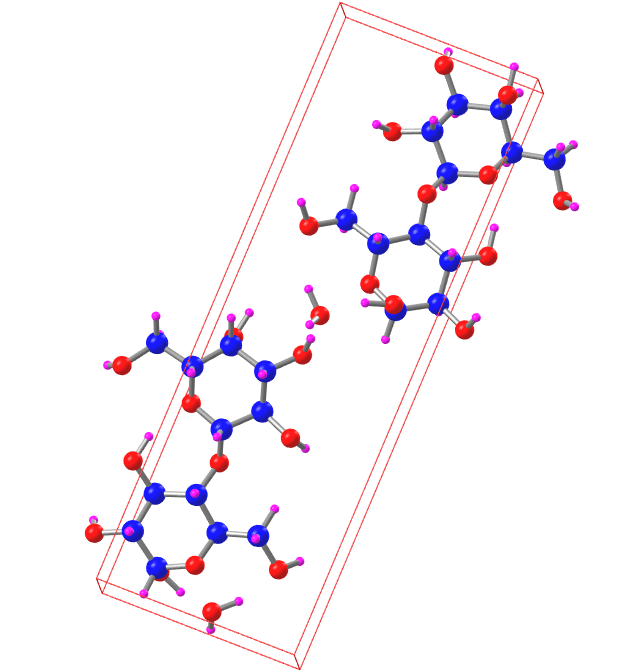
\includegraphics[width=0.6\textwidth]{Figures/Analysis/IVDW/aLM_struct_UC_2.png}
    \captionsetup{font = footnotesize, justification = centering}
    \caption[The Unit Cell of \(\alpha\)-Lactose Monohydrate]{The Unit Cell of \acrshort{alm}. Key: C - Blue; O - Red; H - Magenta.}
    \label{fig:aLM_Structure}
\end{figure}

\section{Method}
\subsection{Experimental Spectrum}
\begin{figure}[bh!]
    \centering
    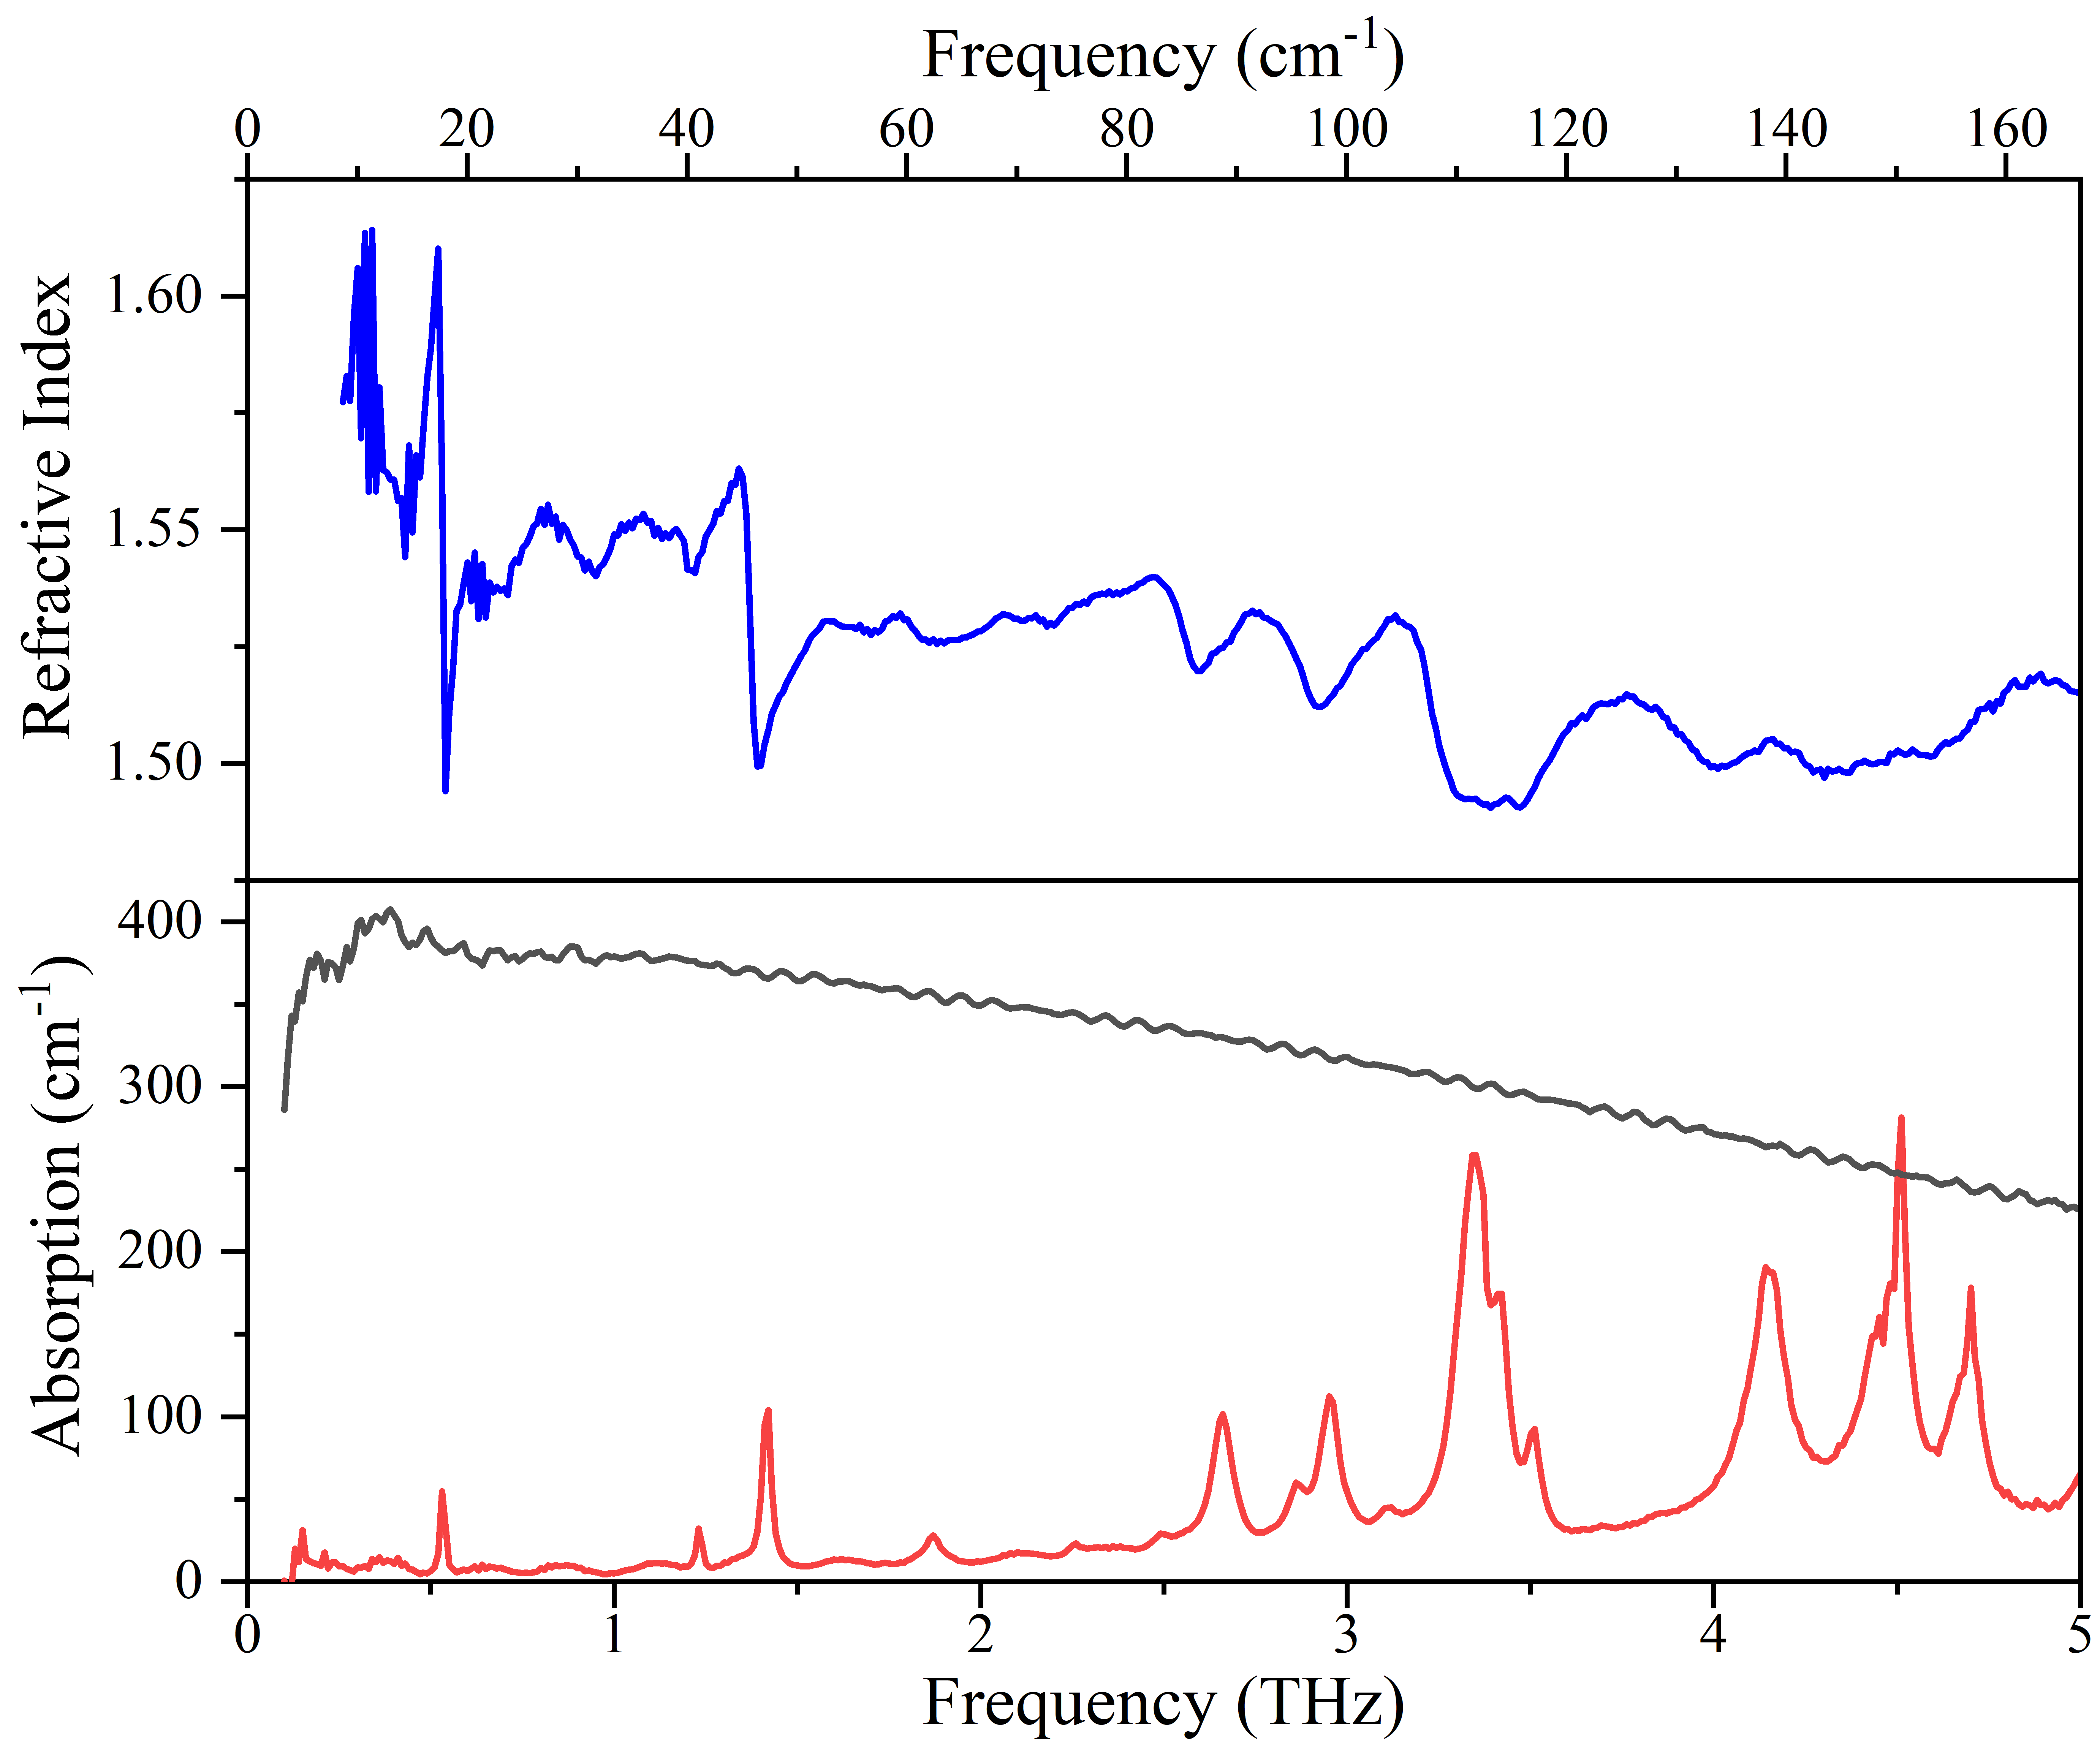
\includegraphics[width=0.6\textwidth]{Figures/Spectra/AbsRefInd.png}
    \captionsetup{font = footnotesize, justification = centering}
    \caption[The THz Absorption Spectrum and Refractive Index of \(\alpha\)-Lactose Monohydrate]{The \acrshort{thz} absorption spectrum of an ${\alpha}$LM pellet in a 10\% mass ratio with \acrshort{ptfe}, taken at \SI{4}{K}. The dynamic range of the spectral measurement is shown and crosses the absorption at approximately \SI{4.5}{\acrshort{thz}}. Finally, the top pane shows the frequency\nobreakdash-dependent refractive index of the sample. It can be seen that the large changes in refractive index correspond to the peaks in the absorption spectrum.}
    \label{fig:AbsRefInd}
\end{figure}

\Cref{fig:AbsRefInd} shows the experimental \acrshort{thz} absorption spectrum and refractive index of a pellet of \acrshort{alm} and \acrshort{ptfe} in a 1:9 mass ratio, along with the dynamic range of the \acrshort{thz}measurement. This spectrum was taken at \SI{4}{K} on  System~1, the \acrshort{tds} system described in \Cref{subsec:tdssystems}. As discussed in \Cref{ch:exp_theory}, the dynamic range represents the ratio of the highest detected signal component and the noise floor of the system. This means that after the point at which the absorption and dynamic range intersect, the central frequency and maximum absorption of each peak cannot be accurately determined. Two peaks in this range have been included to determine the impact of the corrections on some higher frequency modes as updates to the \acrshort{tds} system and its generation and detection methods will allow accurate determination of these spectral parameters in the future. 

\subsection{Density Functional Theory Calculation Parameters}
As described in \Cref{ch:dft_theory}, most starting structures for these calculations are obtained from a single\nobreakdash-crystal \acrshort{xrd} pattern. All structural optimisations and spectral calculations were performed on the \acrshort{alm} structure measured at \SI{150}{K} by Smith \textit{et al.} \DIFdelbegin \DIFdel{~}\DIFdelend \cite{Smith2005}, obtained from the Cambridge Crystallographic Database \DIFdelbegin \DIFdel{~}\DIFdelend \cite{Groom2016}. The k\nobreakdash-point grid and plane wave cut-off energy were converged using the method previously described in \Cref{ch:dft_theory}, resulting in a Monkhorst\nobreakdash-Pack k\nobreakdash-point grid of 715 with a total of 35 k\nobreakdash-points and a cut\nobreakdash-off energy of \SI{900}{eV}. A separate geometry optimisation and calculation of the vibrational properties was performed for each \acrshort{dc}, according to the method described in \Cref{sec:DFTheory}. The post\nobreakdash-processing of these \acrshort{dft} calculations to construct a vibrational absorption spectrum is performed using PDielec \DIFdelbegin \DIFdel{~}\DIFdelend \cite{Kendrick2016} using the settings described below. Each scan has a resolution of \SI{0.2}{cm^{-1}} and the peak widths were matched to their experimental \acrshort{fwhm}s. This is discussed further in \Cref{subsec:ch4_spectra}. 

% Figure here for placement purposes.
\begin{figure}
\centering
\begin{subfigure}{1\textwidth}
    \centering
    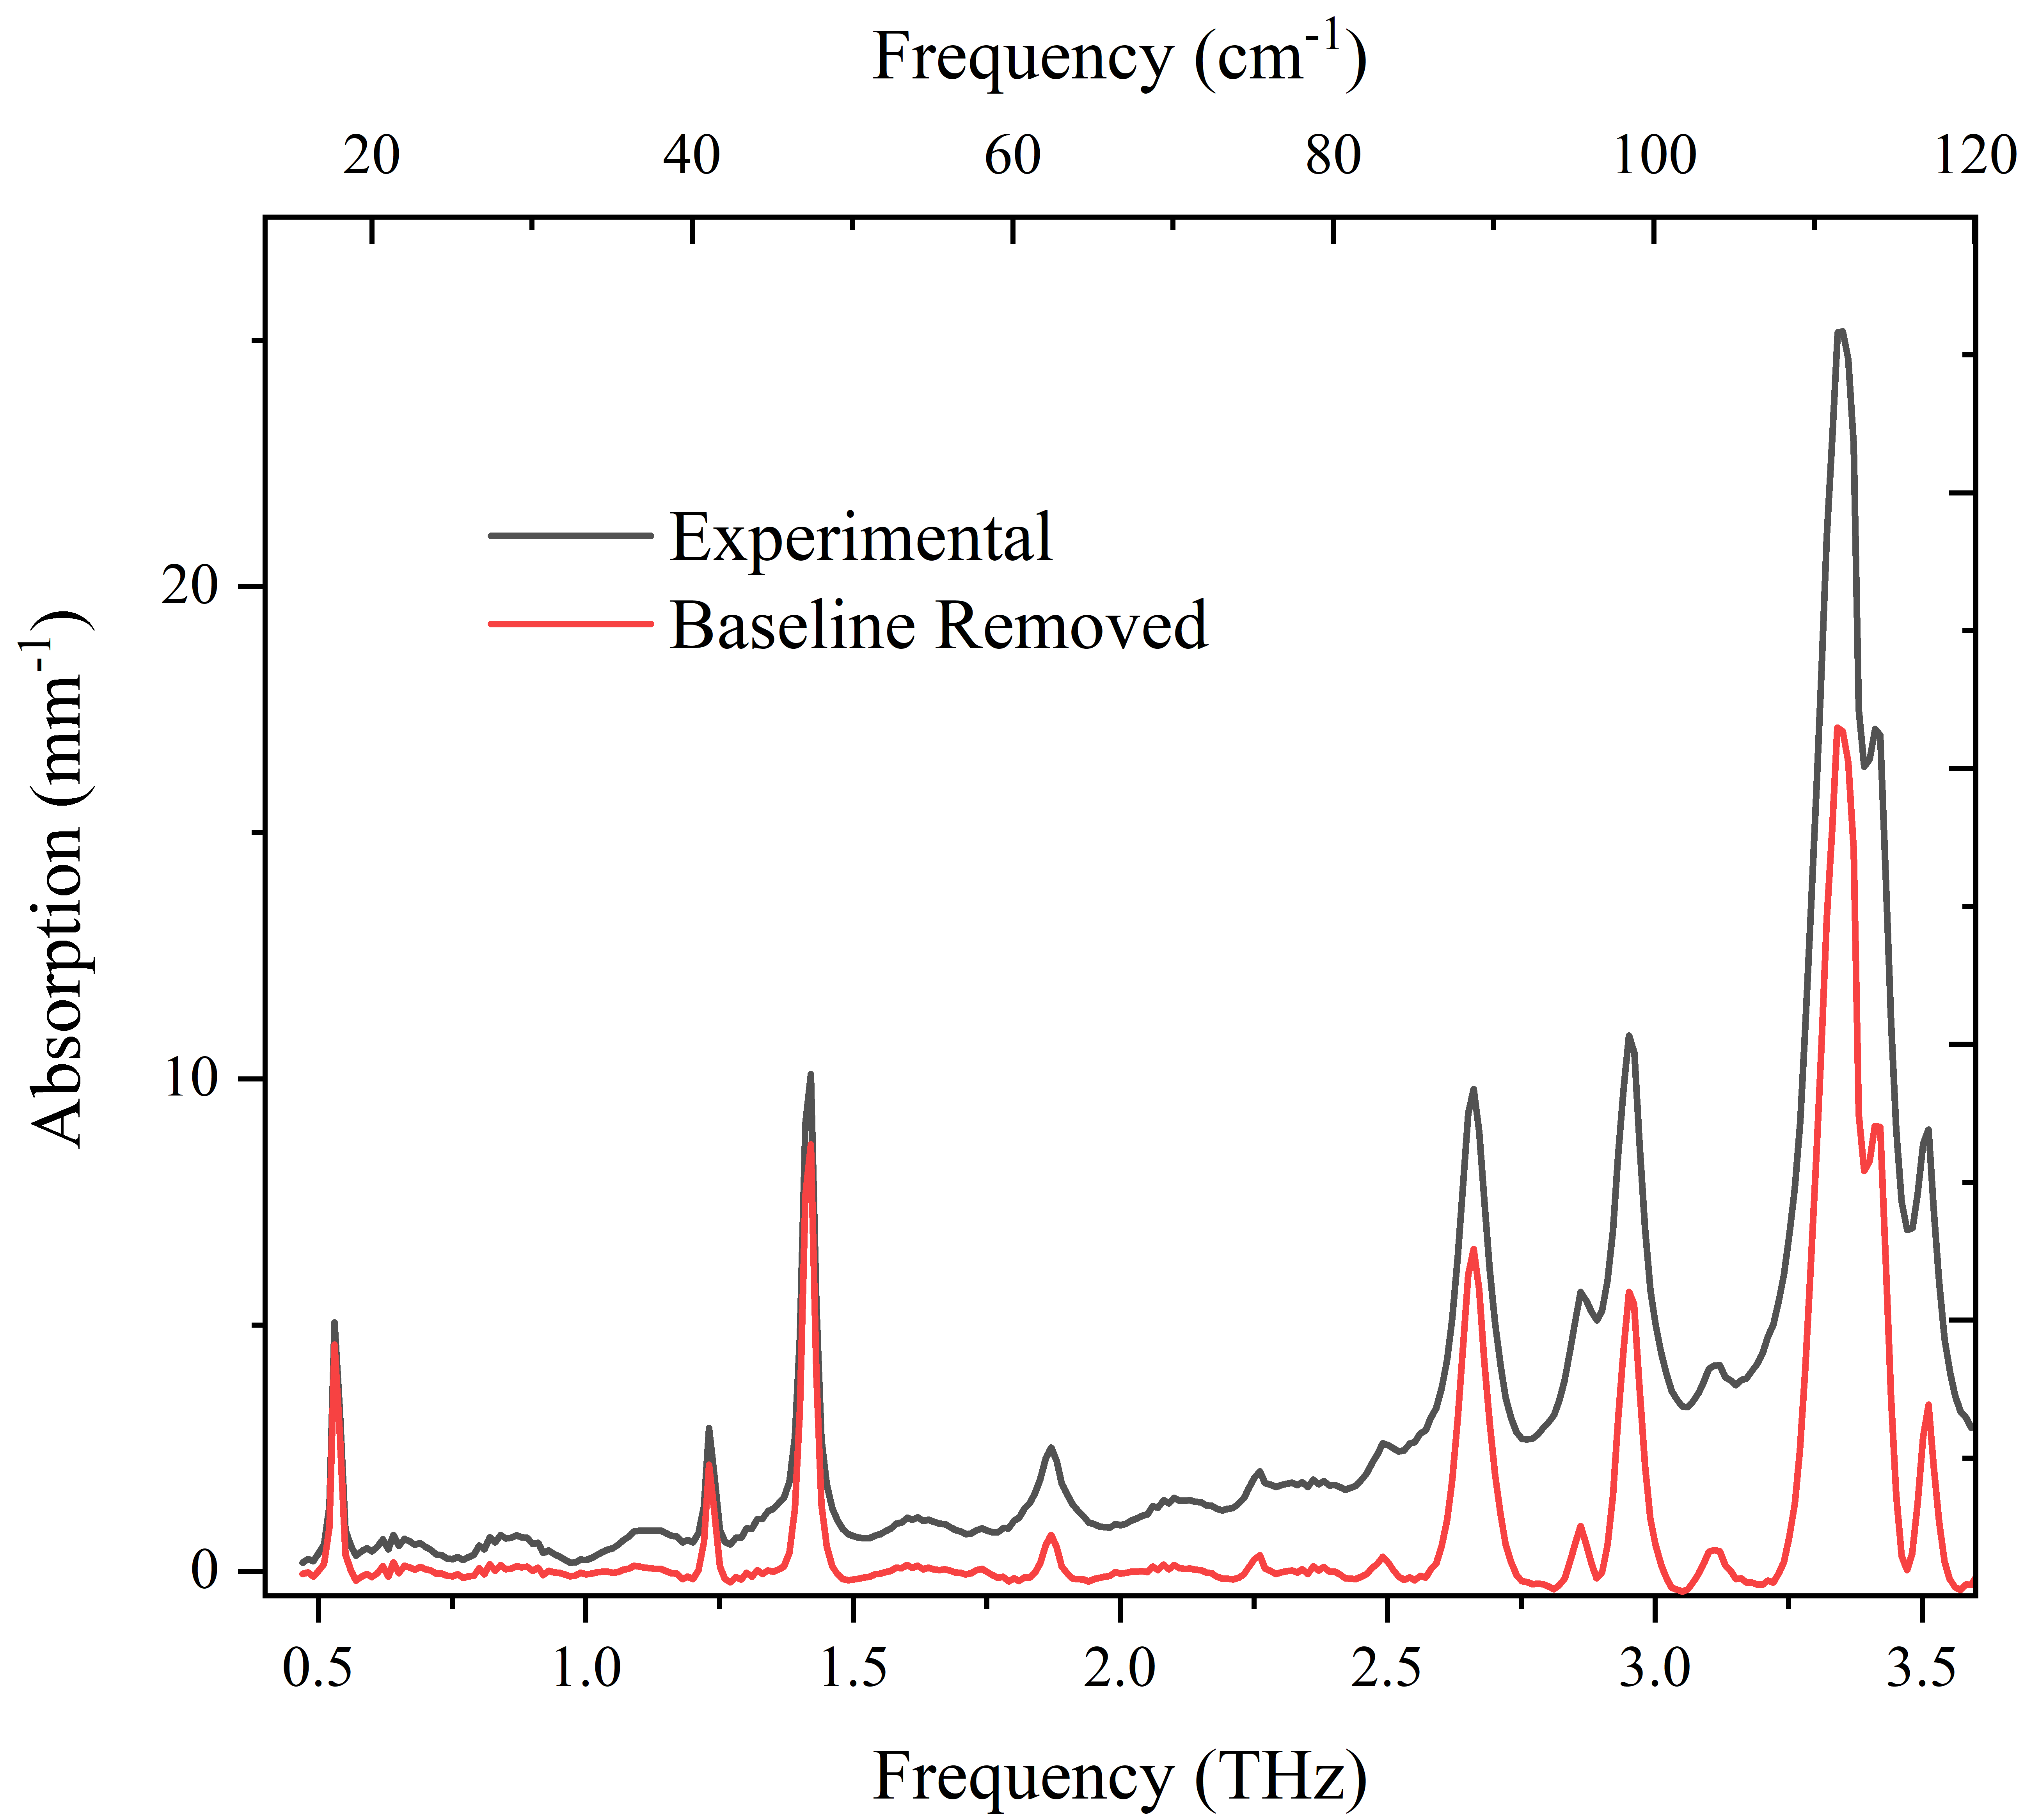
\includegraphics[scale=0.5]{Figures/Spectra/ExpVsBaselineG.png}
    \caption{Removal of background absorption for better peak analysis.}
    \label{fig:aLM_abs_baseline}
    \vspace{5 mm}
\end{subfigure}
\begin{subfigure}{1\textwidth}
    \centering
    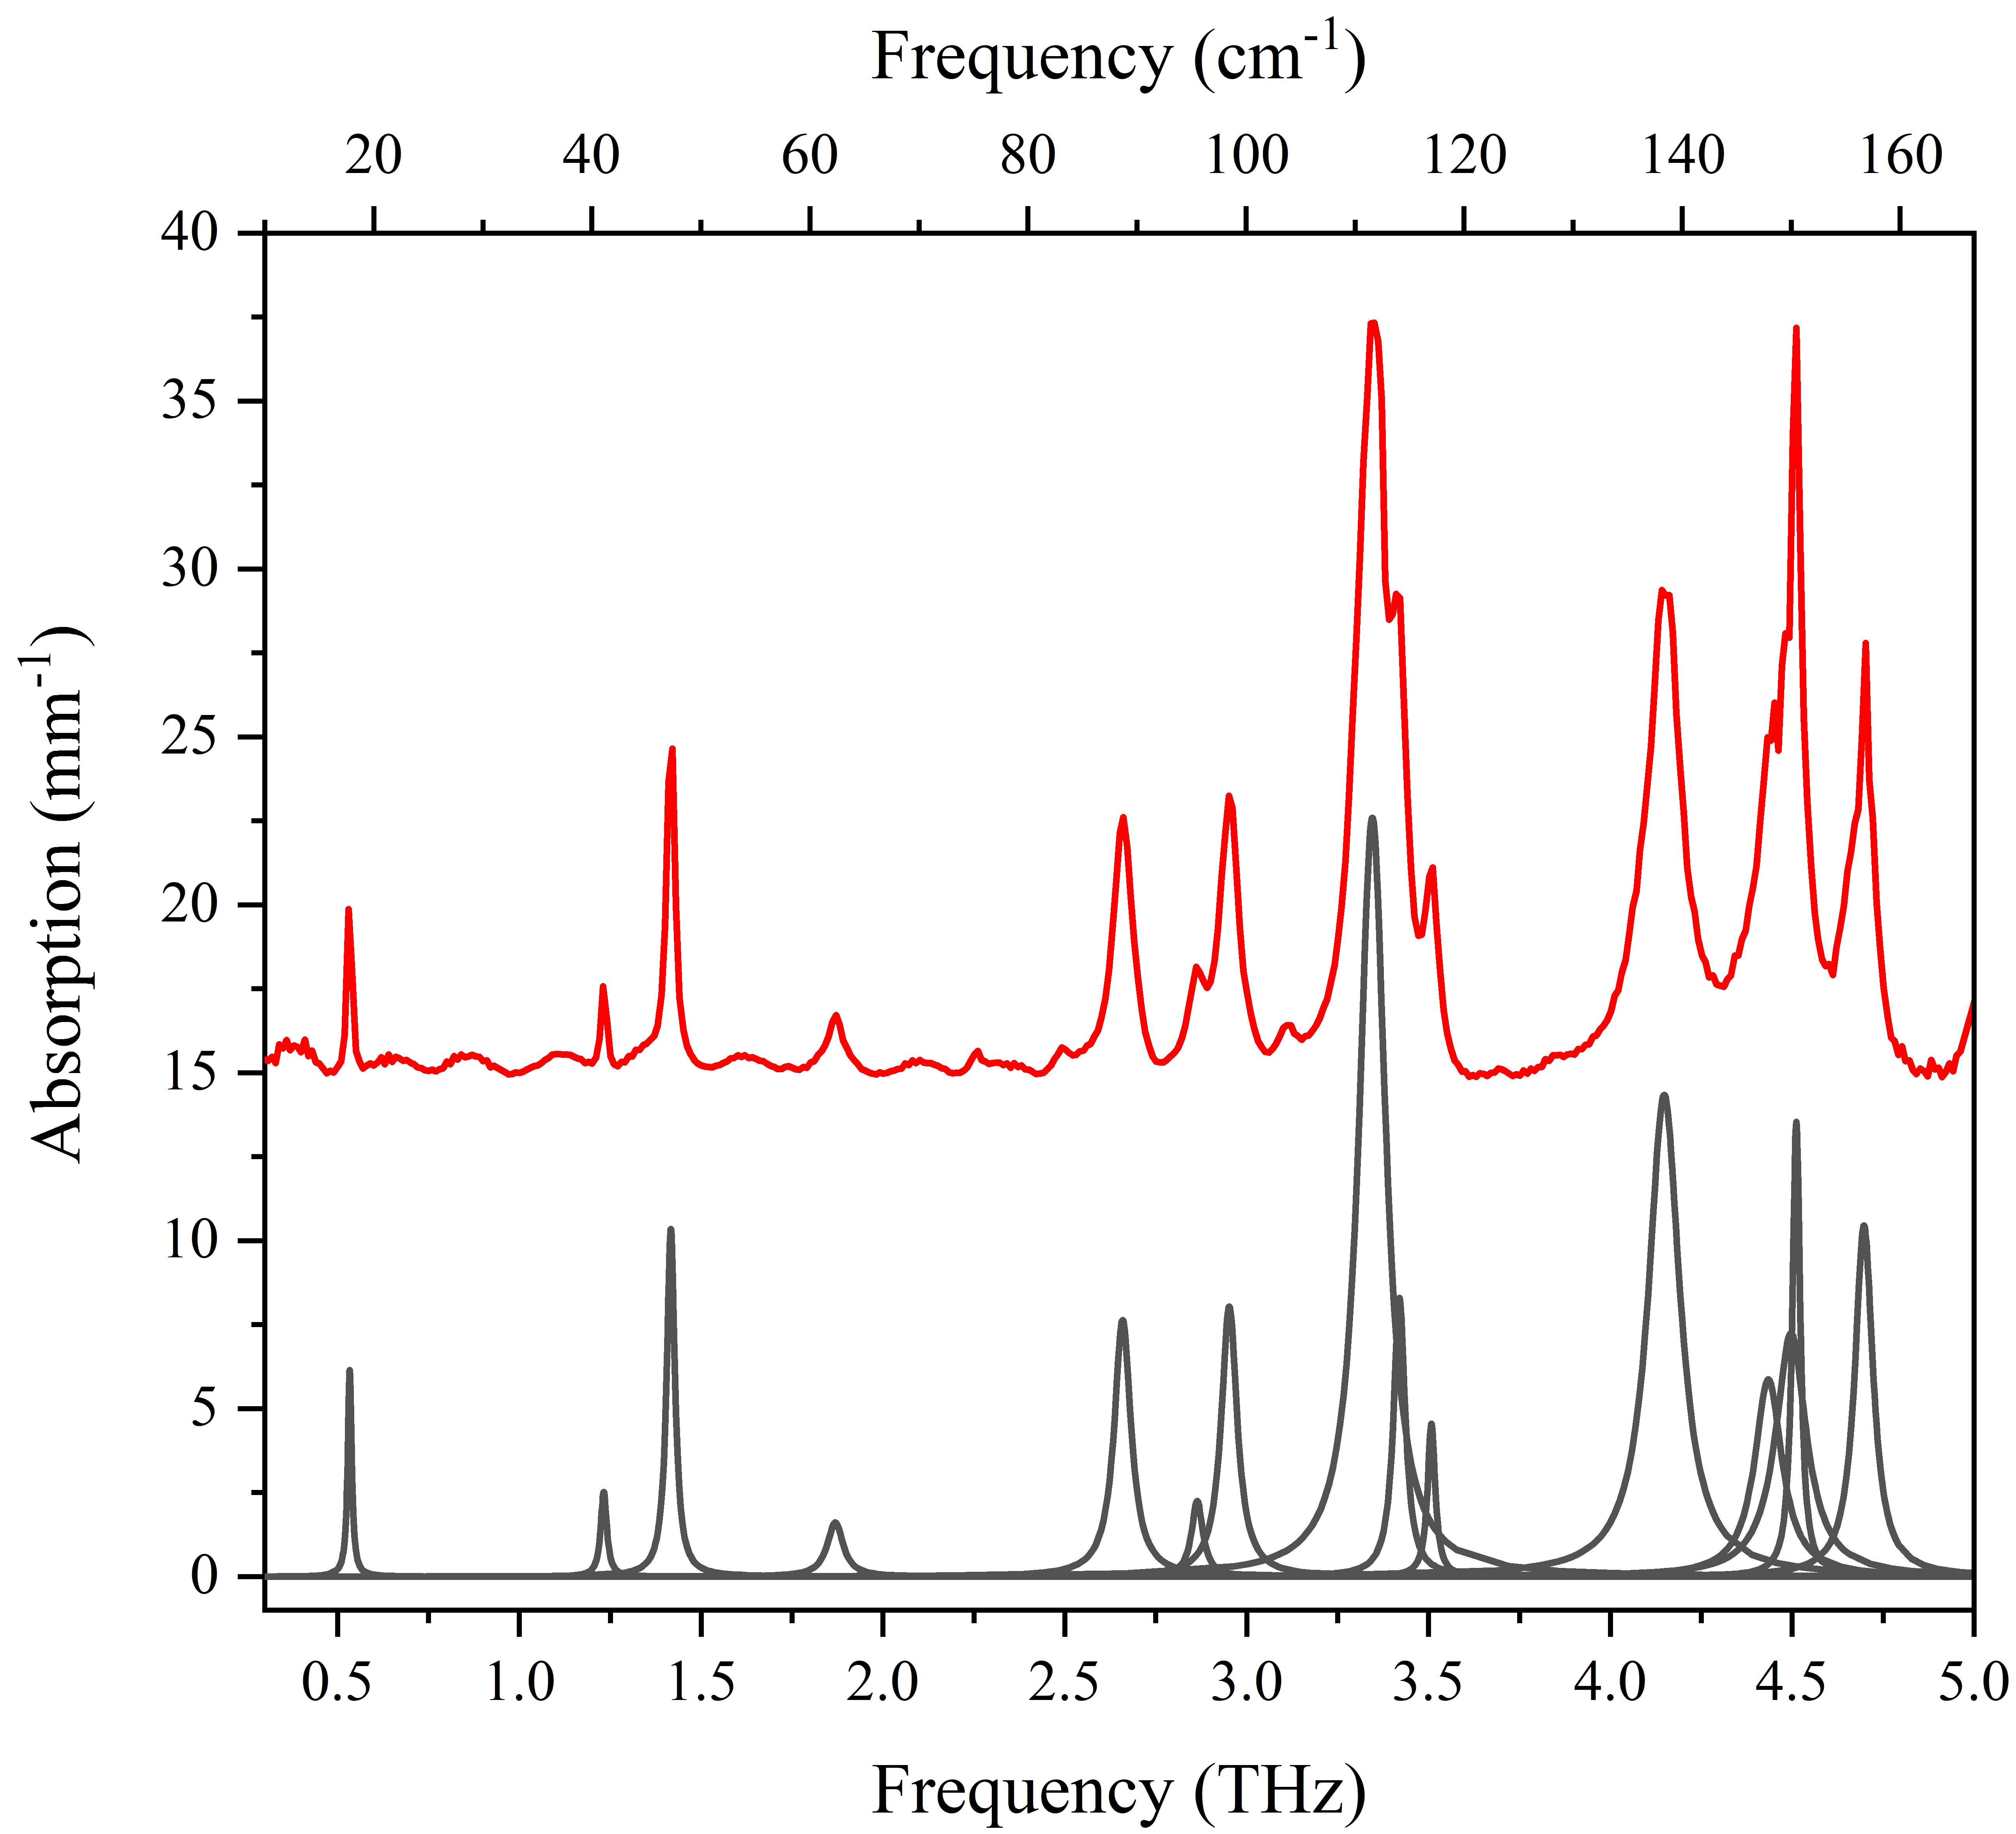
\includegraphics[scale=0.5]{Figures/Spectra/LorentzPeaksG.png}
    \caption{The Lorentzian peaks used to model the experimental peaks and extract the \acrshort{fwhm}s, shown in black. The experimental data with its background absorption subtracted is shown for comparison in red and is offset by \SI{15}{cm^{-1}} for clarity.}
    \label{fig:aLM_abs_lorentz}
\end{subfigure}
\captionsetup{font = footnotesize, justification = centering}
\caption[Extraction of Experimental Peak Widths]{The process of extracting peak properties from the experimental \acrshort{thz} absorption spectrum.}
\label{fig:peak_widths}
\end{figure}

\section{Analysis and Results}
\subsection{Effect of Dispersion Correction on the Calculated Terahertz Absorption Spectrum}
\label{subsec:ch4_spectra}
As discussed in \Cref{subsec:pdielec}, only the individual mode frequencies and intensities are produced in the calculation. To compare these to an experimental spectrum, the modes must be assigned a peak\nobreakdash-width and the absorption values for the frequencies between these peaks must be interpolated. This was done using PDielec, where after trialling each effective medium theory for the best correlation with experiment, Bruggerman's \DIFdelbegin \DIFdel{~}\DIFdelend \cite{Bruggeman1935} theory was selected in a 10\% ratio by mass with \acrshort{ptfe}. To better account for features such background absorption, which typically results from light being scattered through the sample and manifests as a slowly rising base absorption as frequency increases, air voids were included with a void radius of \SI{13}{\micro\metre} and total volume of 5\%. This value is in near agreement with \DIFdelbegin \DIFdel{~}\DIFdelend \cite{Parrott2009} who first introduced air inclusions into calculations for similar pellets. The rising background absorption that increases with frequency is chosen with the aim of increasing calculated and experimental spectral correlation.

\Cref{fig:peak_widths} shows the experimental \acrshort{thz} absorption spectrum with the background removed and the Lorentzian peaks that were used to calculate the peak widths for use in constructing the theoretical spectrum. These peak widths are shown in \Cref{tab:exp_peak_widths}. These were obtained using Origin's Peak Finder function with the background first being removed using the Asymmetric Least Squares Smoothing algorithm where an asymmetric factor of 0.001, a threshold of 0.001, a smoothing factor of 4 and 10 iterations were used. The peaks were found using the 1st derivative method. Each experimental peak width was matched to its corresponding calculated peak and while generally, across all calculations, it was clear which experimental peak corresponded to a given calculated peak, this was sometimes challenging and so the peak was also matched using its intensity. Assignment of peaks and peak widths has been consistent across each \acrshort{dc}s calculation. 

\begin{table}
\centering
\begin{tabular}{@{}cccc@{}}
\toprule
Mode & Mode Frequency / cm\({^{-1}}\) & Peak Width / cm\({^{-1}}\) & Peak Height / cm\({^{-1}}\) \\ \midrule
1 &
17.8 &
0.43 &
6.15 \\

2 &
41.1 &
0.67 &
2.52 \\

3 &
47.2 & 
0.91 &
10.4 \\

4 &
62.3 &
1.77 &
1.61 \\

5 &
88.6 &
1.86 &
7.63 \\

6 &
95.5 &
1.27 &
6.15 \\

7 &
98.4 &
1.76 &
8.04 \\

8 &
111.5 &
2.97 &
22.6 \\

9 &
114.0 &
1.29 &
8.30 \\

10 &
116.9 &
0.84 &
4.55 \\

11 &
138.3 &
3.51 &
14.3 \\

12 &
147.8 &
3.04 &
5.87\\

13 &
149.9 &
3.42 &
7.24 \\

14 &
150.4 &
0.87 &
13.5 \\

15 &
156.6 &
2.02 &
10.4 \\ \bottomrule
\end{tabular}
\captionsetup{font = footnotesize, justification = centering}
\caption[The Properties of the Lorentzian Peaks used to Model the Experimental Terahertz Absorption Peaks of \(\alpha\)-Lactose Monohydrate]{The properties of the Lorentzian peaks used to model the experimental \acrshort{thz} absorption peaks of \(\alpha\)-Lactose Monohydrate shown in \Cref{fig:aLM_abs_lorentz}.}
\label{tab:exp_peak_widths}
\end{table}

The calculated spectra both with and without a \acrshort{dc} are shown in \Cref{fig:vdw_results_all}. It is evident that not using a \acrshort{dc} drastically affects the spectral features above \SI{3.5}{THz}, but below this shows some agreement with the other corrections. However, the differences that are present show that it is not acceptable to do these calculations without using a \acrshort{dc} if experimentally comparable results are required. The D2 correction seems to have slightly overestimated the modes above \SI{4}{THz}, whilst the remaining corrections are very similar in terms of mode frequencies and shape. From initial inspection, D3 appears to match the experimental spectrum the best although the \acrshort{ts} correction also represents the experimental reasonably well. Comparison of the positions of the first and most intense resolved peak between calculated and experimental spectra is one method of quickly assessing how well a calculation has performed and these are detailed in \Cref{tab:calc_exp_peaks}. The first peak for \acrshort{alm} is particularly important owing to it not shifting with temperature and its small width. Here, the D3 correction matches experiment most closely and is the only calculation to produce a mode frequency within the frequency resolution of System~1 but the \acrshort{ts} correction produces the best experimental correlation with the largest resolved peak. The largest peak in the spectrum is not used as owing to the dynamic range of the system, the true experimental mode frequency is not known accurately. Ideally, this peak would be used as it will dominate any spectral optimisation and correlation.

\begin{figure}
\centering
\begin{subfigure}{1\textwidth}
    \centering
    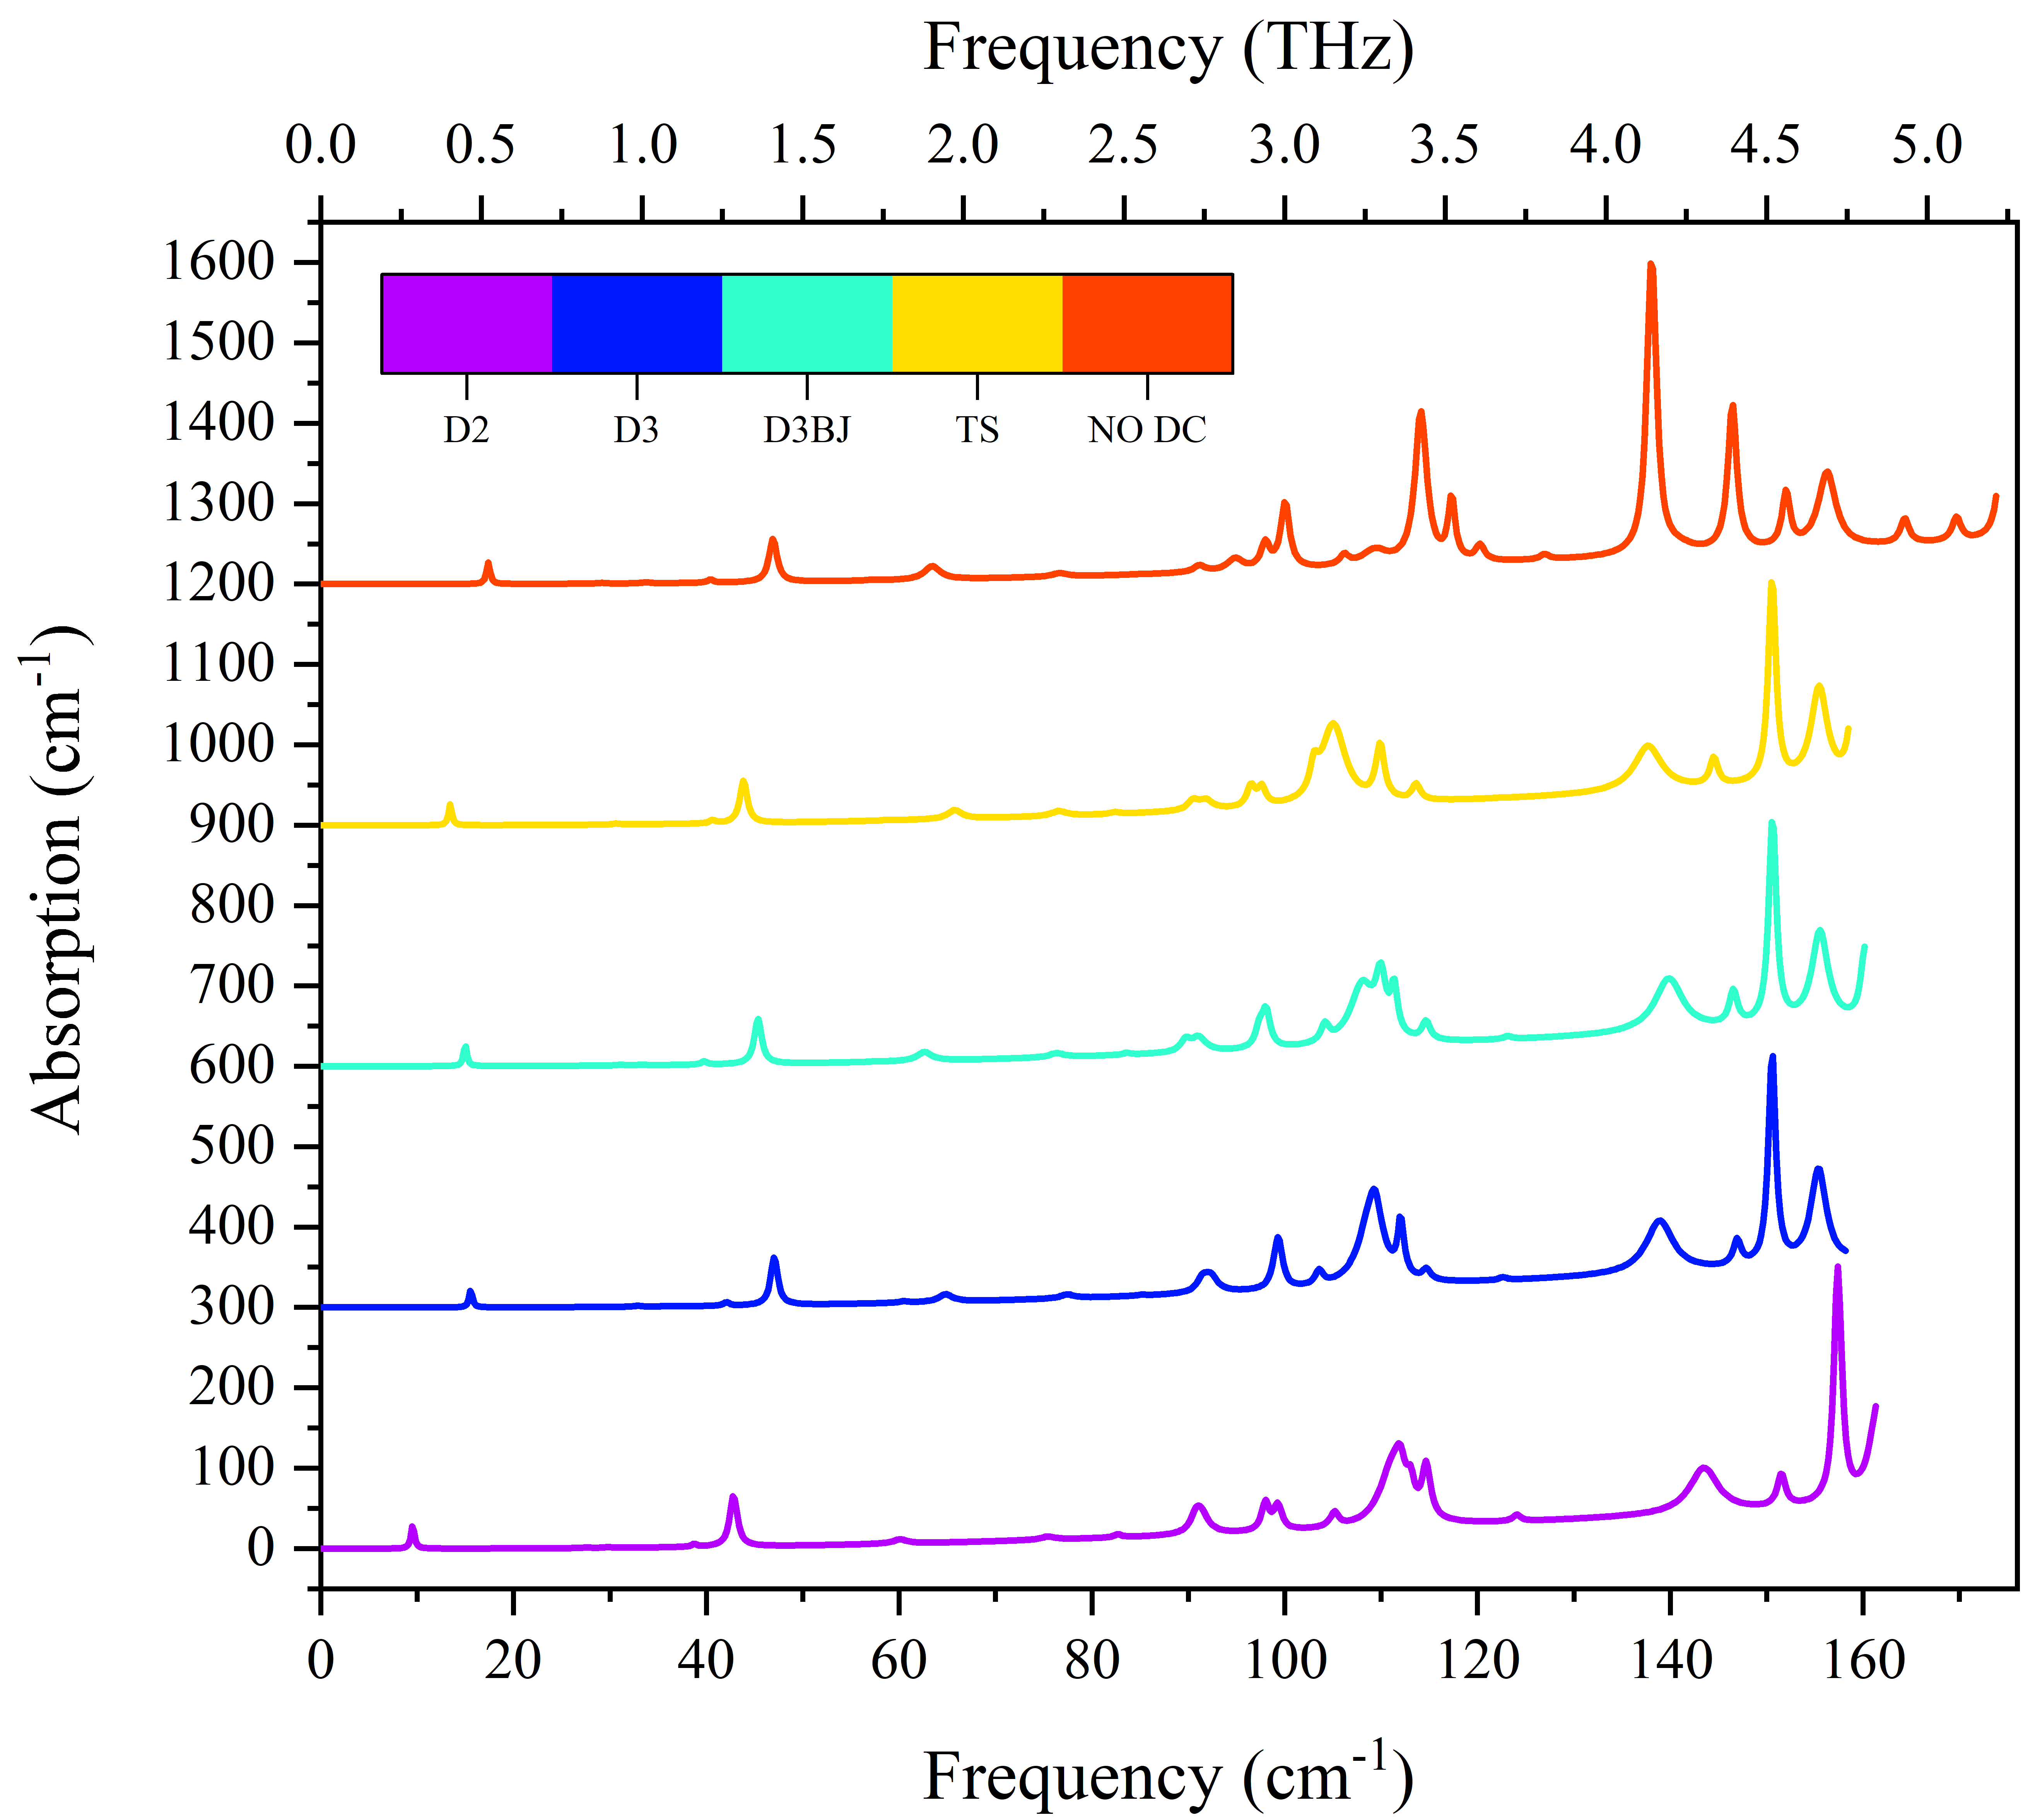
\includegraphics[scale=0.49]{Figures/Spectra/SpecCompScG.png}
    \caption{The calculated \acrshort{thz} absorption spectrum for each correction. All of the corrections have had largely similar effects on the peak positions whereas having no correction causes a large difference in the final spectrum. }
    \label{fig:vdw_results_all}
\end{subfigure}
\begin{subfigure}{1\textwidth}
    \centering
    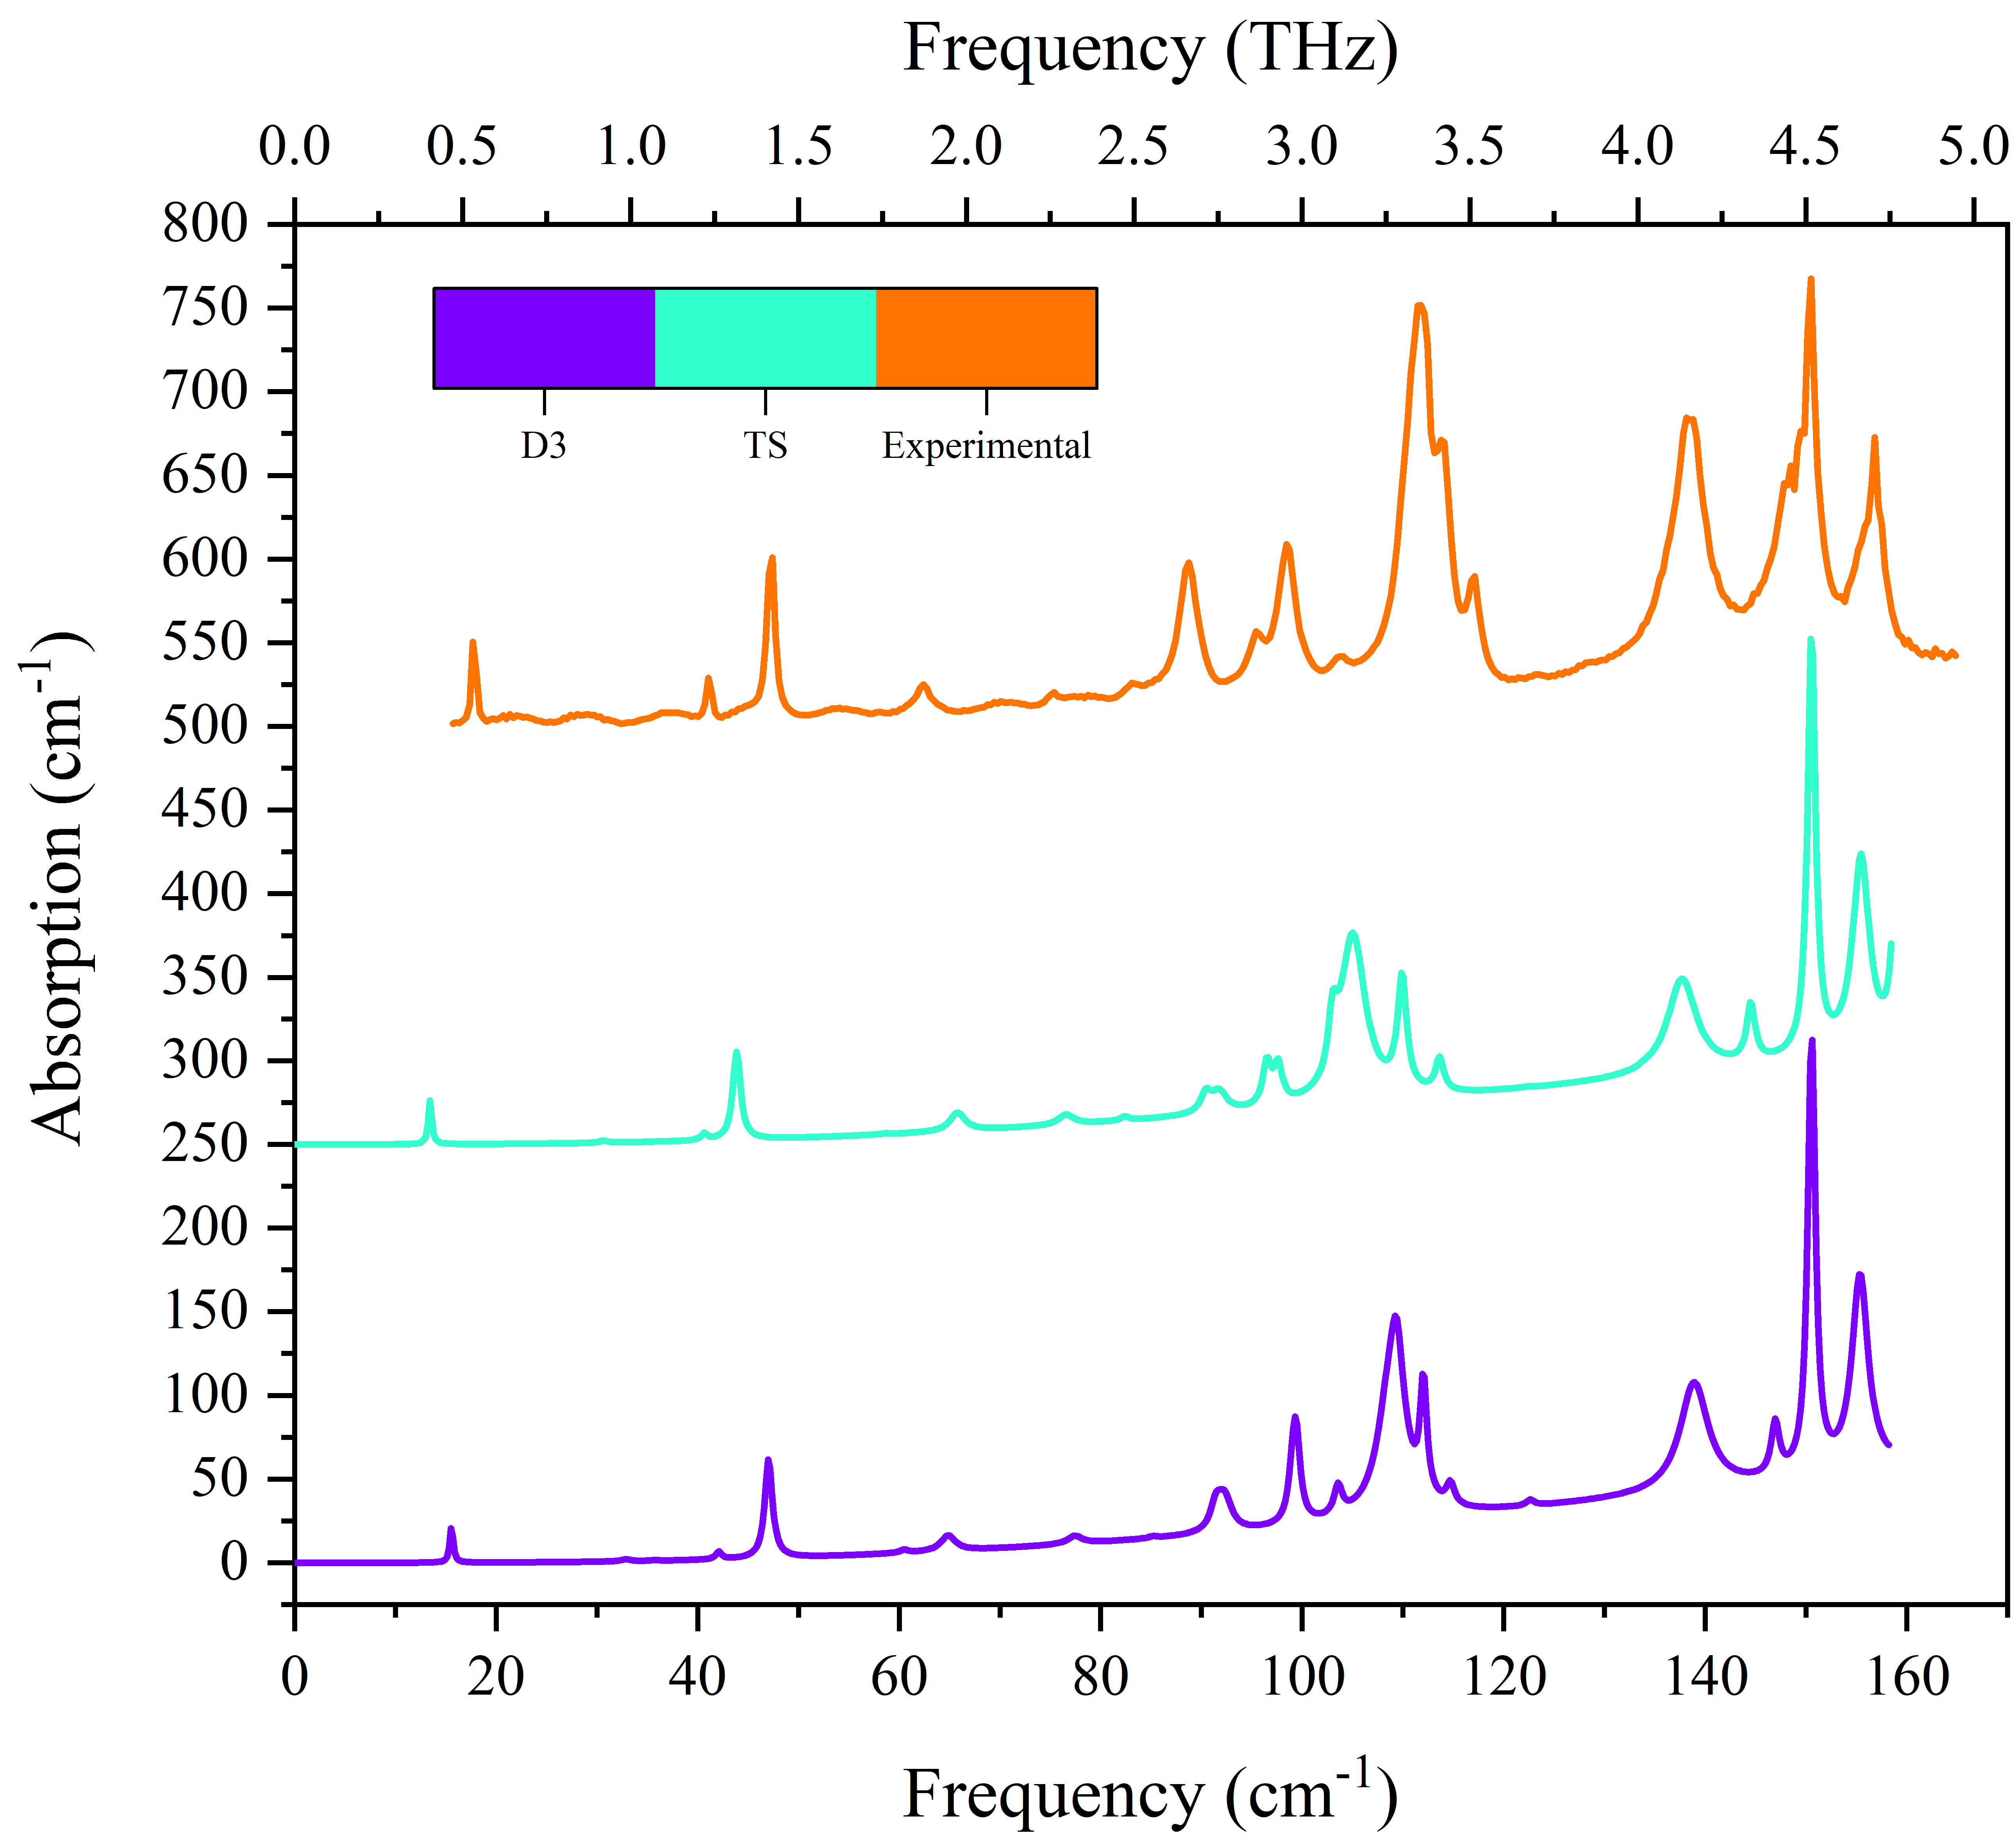
\includegraphics[scale=0.49]{Figures/Spectra/ExpCompG.png}
    \caption{The \acrshort{ts} and D3 spectra compared to the experimental spectrum. The D3 correction is evidently the most similar to the experimental spectrum.}
    \label{fig:exp_d3_ts}
\end{subfigure}
\captionsetup{font = footnotesize, justification = centering}
\caption[The Calculated Terahertz Absorption Spectra for each Dispersion Correction and the Experimental Spectrum]{The final spectra for each correction and the experimental spectrum. As expected, the spectrum where no correction was used is not acceptable but the D3\acrshort{bj} correction also did not perform ideally. The D3 spectrum appears to have most of the spectral features in the correct place below the noise cutoff at \SI{4.5}{\acrshort{thz}}}
\label{fig:vdw_results}
\end{figure}

The method chosen to compare experimental and calculated spectra was to calculate the normalised cross\nobreakdash-correlation coefficient \DIFdelbegin \DIFdel{~}\DIFdelend \cite{Kendrick2020}. This is where the signals are normalised and one signal is shifted along an axis, in this case frequency, and the overlap between these signals is calculated for each shift using integration. The signals are normalised using the equation:

\begin{equation}
A_{norm}(i) = \frac{A(i) - A_{mean}}{\sqrt{n}\sigma(A)}
\end{equation}

Where \(A_{norm}(i)\) is the normalised value in row \(i\), \(A(i)\) is the un\nobreakdash-normalised value in row \(i\), \(A_{mean}\) is the average signal value, \(n\) is the number of rows in the dataset and \(\sigma\) is the standard deviation of the whole dataset. The size of this integral is recorded as a function of the value of the shift and the maximum value of this overlap indicates where the signals are most similar. This maximum can then be used to compare the relative success of each correction. The cross\nobreakdash-correlation can take values of -1 to 1, where 0 is no correlation and a value of 1 would mean identical signals. The shift where maximum overlap occurred has also been recorded. This attempts to correct for any systematic error in the calculations but large values indicate a worse result.

%I think here for placement purposes but not 100% sure.
\begin{table}
\centering
\begin{tabular}{@{}ccc@{}}
\toprule
Correction            & First Peak Frequency / cm${^{-1}}$           & Largest Resolved Peak Frequency / cm${^{-1}}$      \\ \midrule
None &
  21.54 &
  109.96 \\
D2 &
  16.38 &
  115.72 \\
D3 &
 18.01 & 
 113.87 \\
D3\acrshort{bj} &
  20.08 &
  112.68 \\
TS &
  19.77 &
  111.13 \\
Exp &
  17.60 &
  111.79 \\ \bottomrule
\end{tabular}
\captionsetup{font = footnotesize, justification = centering}
\caption[The First and Largest Resolved Calculated and Experimental Spectral Peaks]{The first and largest resolved calculated and experimental spectral peaks. For the first peak, the D3 correction has the closest value whilst the \acrshort{ts}correction has the closest value to the largest resolved peak}
\label{tab:calc_exp_peaks}
\end{table}

PDielec also allows frequency scaling, where the mode frequencies are multiplied by a scaling factor, which is commonly used to crudely incorporate anharmonic effects into the system that is not incorporated during the calculation. For each \acrshort{dc}, these values were optimised to maximise correlation between experiment and calculation. The effect of these corrections is shown in \Cref{fig:scaling}, where it can be seen that a majority of the peaks align better with their experimental counterparts after scaling. This can cause small over\nobreakdash-corrections in some cases, such as for the group of three peaks at \SI{115}{cm^{-1}}, however the overall spectrum is better represented. At these low frequencies, the frequency scaling has a much smaller effect on the correlation than the frequency shift but when considering the mid\nobreakdash-\acrshort{ir} as well, scaling can have a much larger effect. Additionally, the \acrfull{rms} error is also calculated which the average difference between the correlated and experimental values. An increase in correlation does not necessarily result in a decrease in \acrshort{rms} error. Both values for the original and optimised calculated spectra are presented in \Cref{tab:calc_exp_corr}. It is worth noting that the inclusion of the experimental peaks past the dynamic range of the \acrshort{tds} system is likely to reduce comparability between experimental and calculated spectra in this region. This will likely reduce correlation and increase \acrshort{rms} error, however this should be consistent across all corrections.

\begin{figure}[h]
    \centering
    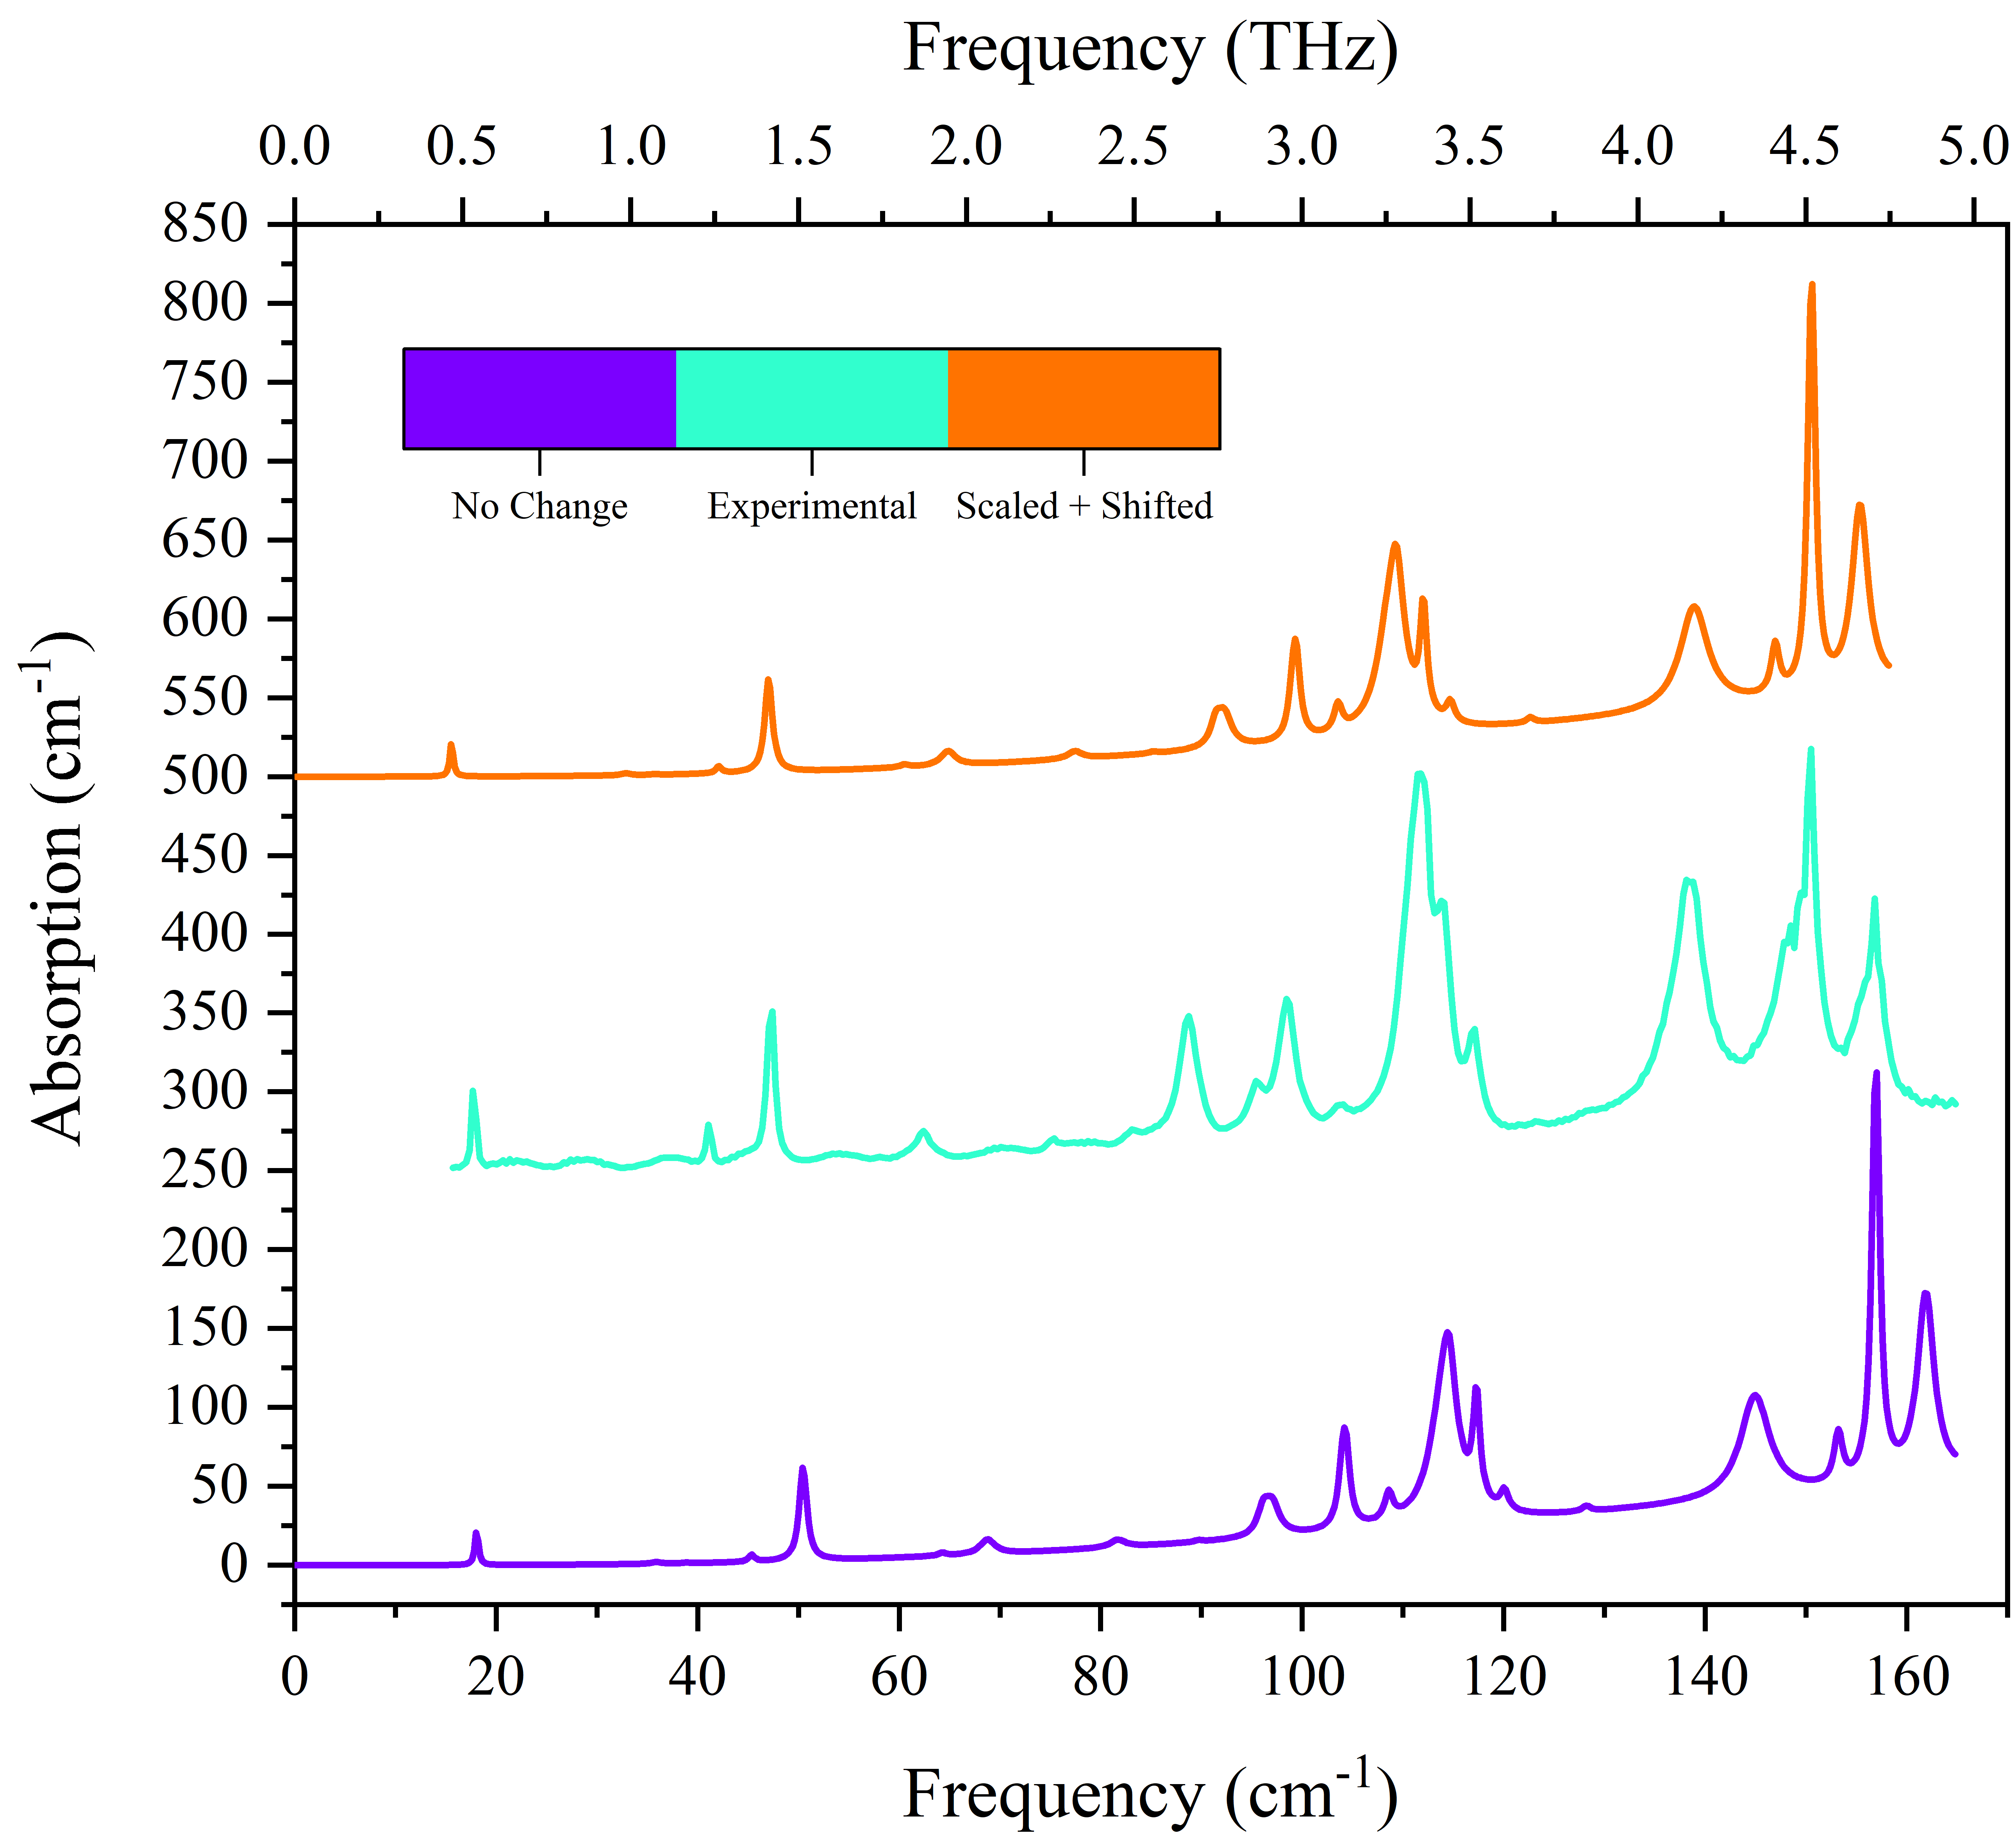
\includegraphics[width=0.7\textwidth]{Figures/Spectra/ScalCompG.png}
    \captionsetup{font = footnotesize, justification = centering}
    \caption[The Effect of Incorporating PDielec Frequency Scaling and Shifting on the D3 Calculated Terahertz Absorption Spectra]{The effect of incorporating PDielec frequency scaling and shifting on the D3 calculated spectra. It can be seen that there is much better agreement with the experimental spectrum after these effects are applied.}
    \label{fig:scaling}
\end{figure}

\begin{table}[h]
\centering
\begin{tabular}{@{}ccccc@{}}
\toprule
Correction & x-Correlation & Magnitude & RMS Error & Frequency \\
 & & of Shift / cm\(^{-1}\) & & Scaling \\ \midrule
None &
  0.6456 &
  1.4 &
  0.164 &
  1.0000 \\
D2 &
  0.7173 &
  -4.8 &
  0.182 &
  1.0000 \\
D3 &
  0.7693 &
  -6.2 &
  0.160 &
  1.0000 \\
D3\acrshort{bj} &
  0.7906 &
  -4.6 &
  0.158 &
  1.0000 \\
\acrshort{ts} &
  0.7136 &
  -6.4 &
  0.149 &
  1.0000 \\ \midrule
None - Scaled &
  0.7063 &
  -6.2 &
  0.208 &
  1.0922 \\
D2 - Scaled &
  0.8032 &
  -8.0 &
  0.175 &
  1.0273 \\
D3 - Scaled  &
  0.8136 &
  -2.0 &
  0.138 &
  0.9721 \\
D3\acrshort{bj} - Scaled  &
  0.7941 &
  -5.2 &
  0.159 &
  1.0033 \\
\acrshort{ts} - Scaled  &
  0.7142 &
  -6.4 &
  0.149 &
  1.0004 \\ \bottomrule
\end{tabular}
\captionsetup{font = footnotesize, justification = centering}
\caption[The Calculated and Experimental Spectral Correlation and Error Before and After Spectral Optimisation]{The calculated and experimental spectral correlation and error before and after spectral optimisation. The D3 correction performs the best for both correlation and \acrshort{rms} error. It was also the only run to have a scaling factor of less than one. This also shows that the optimisation process increases the spectral correlation and should be applied to each future spectrum.}
\label{tab:calc_exp_corr}
\end{table}

As was indicated by inspection and brief analysis of the key mode frequencies, the D3 correction has the highest correlation value and also the lowest \acrshort{rms} error. It also used the lowest frequency shift to do this but was also the only correction where the optimisation process chose a frequency scaling factor of less than one. The D2 correction correlated surprisingly well but required the largest shift and scaling factor indicating the original spectrum was quite flawed. The D3\acrshort{bj} correction was also well correlated but did not represent the central large peaks well. Finally, although the \acrshort{ts} spectrum performed relatively poorly when considering correlation, the spectrum could not be improved with spectral optimisation which may indicate a better representation of the real system. It is worth noting that it also has the second lowest \acrshort{rms} error. It is possible that slight mismatches in the higher frequency modes lowered the correlation for the \acrshort{ts} calculation. 

\begin{figure}[!htb]
    \centering
    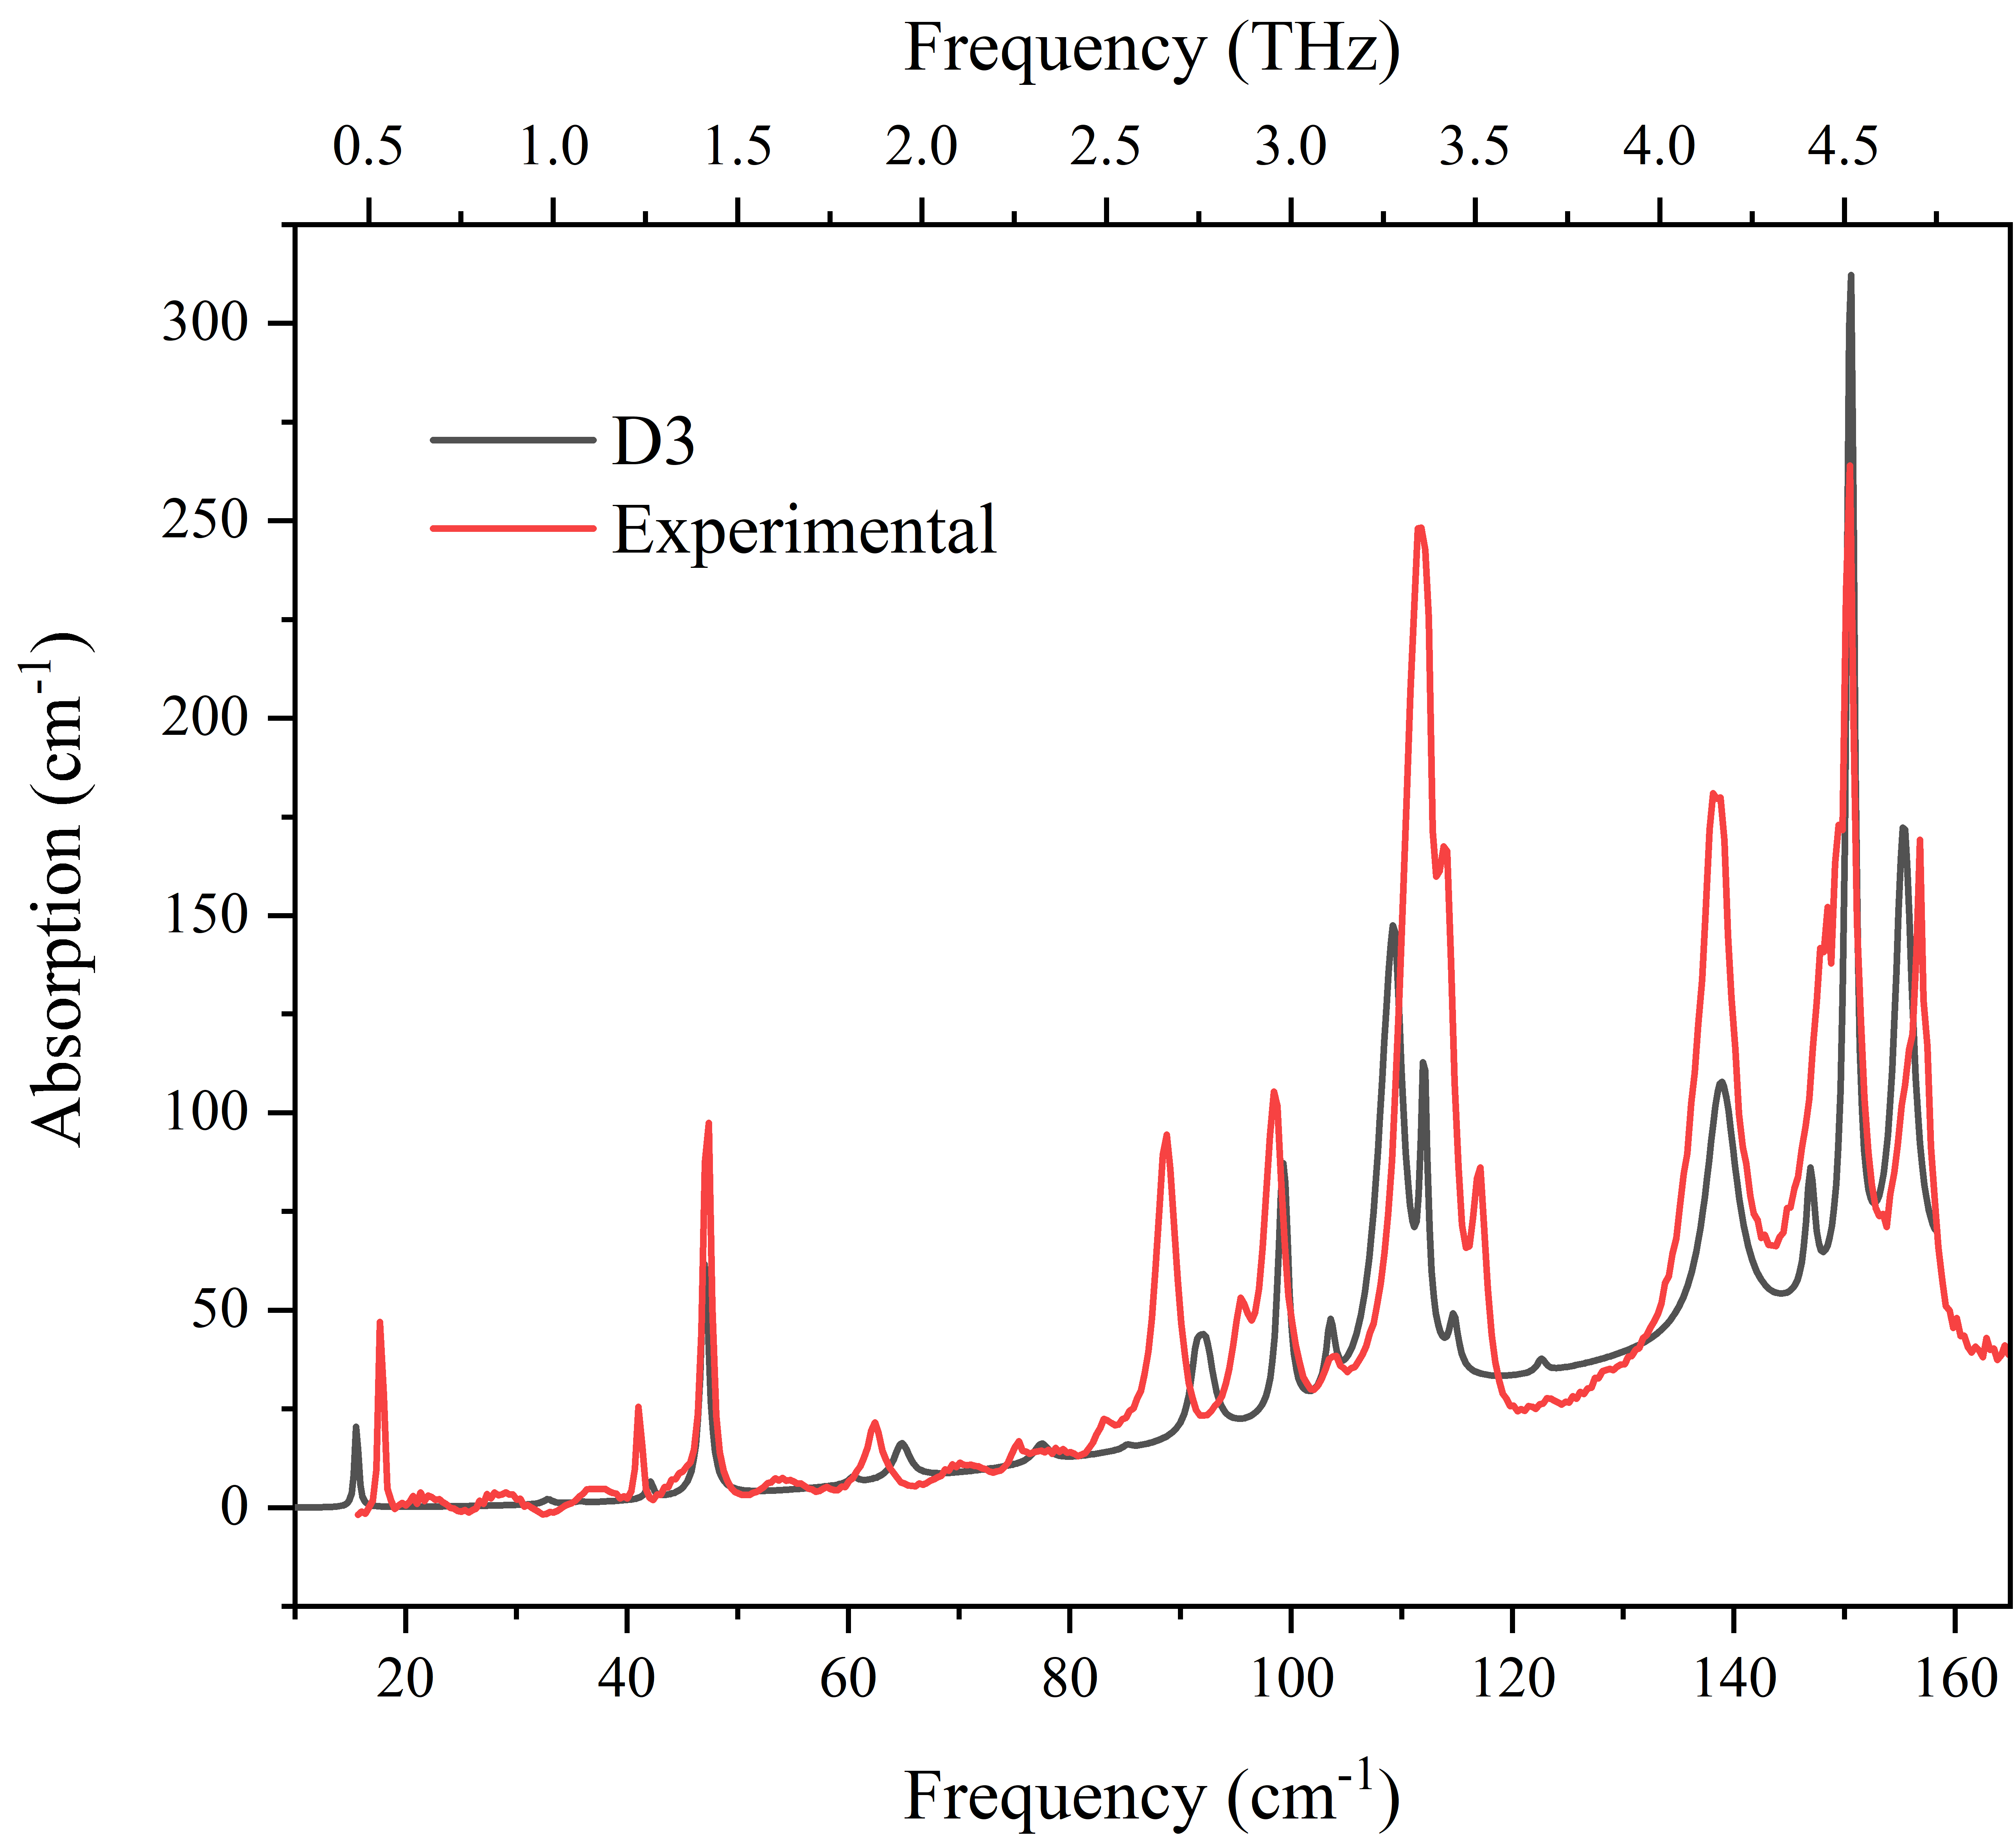
\includegraphics[width=0.7\textwidth]{Figures/Spectra/D3ExpDiffG3.png}
    \captionsetup{font = footnotesize, justification = centering}
    \caption[The Optimised D3 Terahertz Absorption Spectrum alongside the Experimental Spectrum]{The optimised D3 \acrshort{thz} absorption spectrum alongside the experimental spectrum presented in a manner that highlights the differences. Whilst most peaks show very agreements, some of the central peaks are slightly misaligned; particularly the mode at approximately \SI{90}{cm^{-1}}.}
    \label{fig:diff_d3_exp}
\end{figure}

In \Cref{fig:exp_d3_ts}, the D3 and \acrshort{ts} are shown alongside the experimental spectrum. Whilst both bear a good resemblance, the D3 correction demonstrated a superior ability to match the features of the experimental spectrum in this case. Whilst mode frequencies and relative intensities appear to match well, the difference between absolute intensities is approximately a factor of two. The reason for this discrepancy has not yet been identified but may be a result of underestimating the magnitude of the mode's constituent oscillations. However, this \DIFdelbegin \DIFdel{is }\DIFdelend much less important than the relative intensities of the peaks. In \Cref{fig:diff_d3_exp}, the differences between the D3 spectrum and the experimental have been made more apparent. Whilst most modes show excellent agreement, the mode at \SI{90}{cm^{-1}} in the calculated spectrum shows the largest discrepancy. This mode may be more anharmonic than the other modes and this will be analysed further below and in \Cref{ch:qha}.

\begin{figure}[!htb]
    \centering
    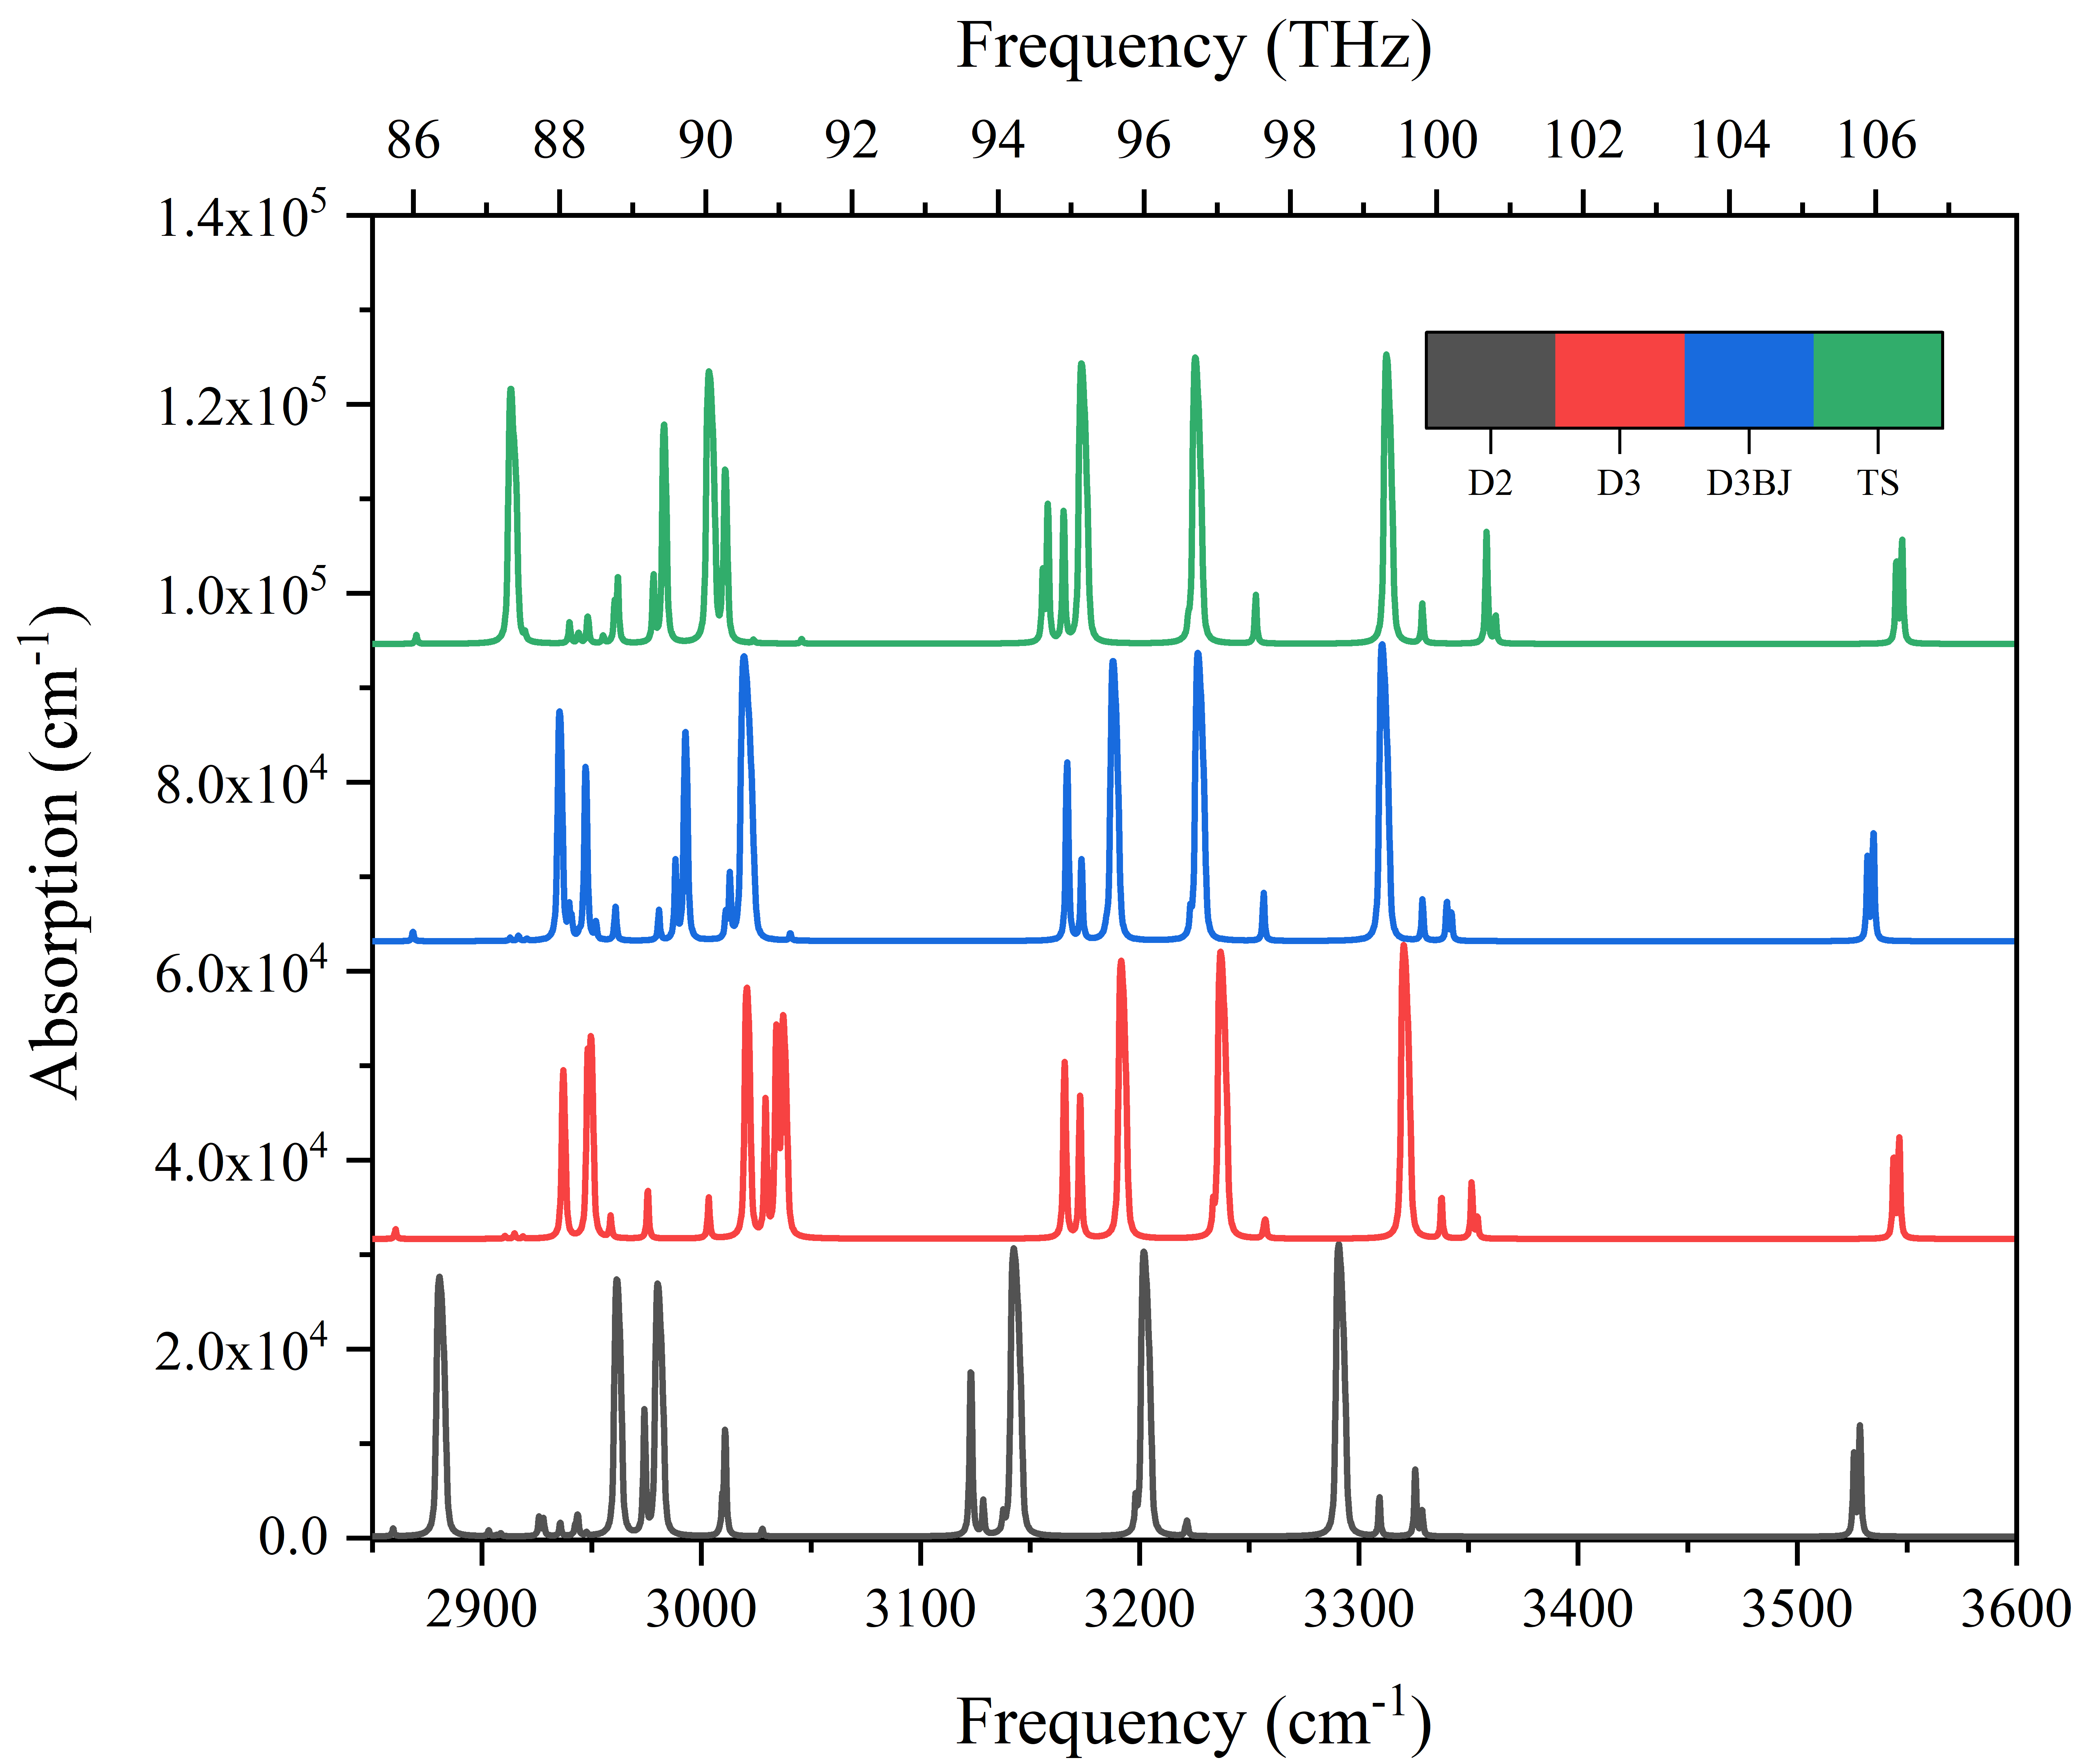
\includegraphics[width=0.7\textwidth]{Figures/Spectra/midIRG.png}
    \captionsetup{font = footnotesize, justification = centering}
    \caption[The Calculated Absorption Spectrum in the Frequency Range Associated with OH Bonds]{The calculated absorption spectrum in the mid\nobreakdash-\acrshort{ir} range that is associated with \(O\)\nobreakdash--\(H\) bonds. While there are minor discrepancies, an experimental spectrum in this region would not have resolved peaks and so these differences are largely irrelevant.}
    \label{fig:midIR}
\end{figure}

As these low\nobreakdash-frequency modes can be difficult to analyse completely, it can be useful to also examine the impact of \acrshort{dc}s on higher frequency modes in the mid\nobreakdash-IR where the motions \DIFdelbegin \DIFdel{involved }\DIFdelend \DIFaddbegin \DIFadd{involves }\DIFaddend are easier to interpret. The mid\nobreakdash-IR spectrum between 2800 and \SI{3600}{cm^{-1}}, the range where OH intramolecular vibrations are typically found, for each correction is shown in \Cref{fig:midIR}. It is clear that whilst the largest modes are fairly close together there is still some differences on mode position and relative intensity, even at this range where the theory is well understood. However, these calculated spectra do not incorporate features such as OH group broadening, where all the peaks shown would be obscured and grouped as either one large or two slightly smaller peaks. This is owing to \DIFaddbegin \DIFadd{to }\DIFaddend H\nobreakdash-bonding between O and H which will cause the mode frequency to have a large distribution. As such, these discrepancies would be largely unimportant when comparing to a real spectrum at this frequency range.

\subsection{Effect of Dispersion Correction on Structural Optimisation}
Although the correlation between experimental and calculated spectra is extremely important, this arises from the aim of understanding the nature of the underlying modes which are much more difficult to predict in the \acrshort{thz} region when compared to the mid\nobreakdash-\acrshort{ir} region. With this in mind, the effect on the structures that each correction had was also investigated. During this investigation, a more complete method for analysing changes between starting and final structures and providing a more complete description of the final structure has been developed.

The \acrshort{dc}s are added to better account for \acrfull{vdw} forces which are extremely important in the stability of organic molecular crystals such as \acrshort{alm}. These forces are responsible for holding the crystal together and so during the structural optimisation, as the algorithm is trying to find the \DIFdelbegin \DIFdel{system's }\DIFdelend \DIFaddbegin \DIFadd{systems }\DIFaddend minimum energy, it is expected that having no correction will cause the unit cell to expand whilst it will contract slightly for the optimisations with a correction. This is likely owing to the temperature the original structure was measured at and that these optimisations do not account for temperature so the small amount of thermal energy even at \SI{150}{K} will alter the atomic positions and unit cell parameters. Without a correction accounting for the intermolecular forces, the energy of the system will be lowered by moving each molecule further apart which will cause the expansion. In \Cref{Fig:UnitCellParams}, the final values for the optimised cell parameters of the five structures that were varied are shown. As expected, the volume decreased for each optimisation with the exception of the run without a correction. With the exception of the \textit{b} unit cell axis for D3, D3\acrshort{bj} and \acrshort{ts}, each axis decreased. This is possibly owing to this being the longest axis by a significant margin and the molecules in the unit cell being aligned with this plane so it has the smallest degree of intermolecular bonding. The D2 correction seems to have overestimated the intermolecular forces and has significantly decreased the unit cell volume. This is also to be expected as D3, D3\acrshort{bj} and \acrshort{ts} were all designed to be improvements to D2. The \(\beta\) angle is the angle between the \textit{a} and \textit{c} unit cell axes and breaks the trend for the D2 correction but owing to the comparative size of the change to the angle itself, this was not considered an issue. These results correlate with the final cell volumes shown in \Cref{fig:volchange}. Owing to the large volume of the unit cell, these changes correspond to a maximum of a 5\% shift in total volume.

\begin{figure}[!htb]
\centering

\begin{subfigure}{0.49\textwidth}
\centering
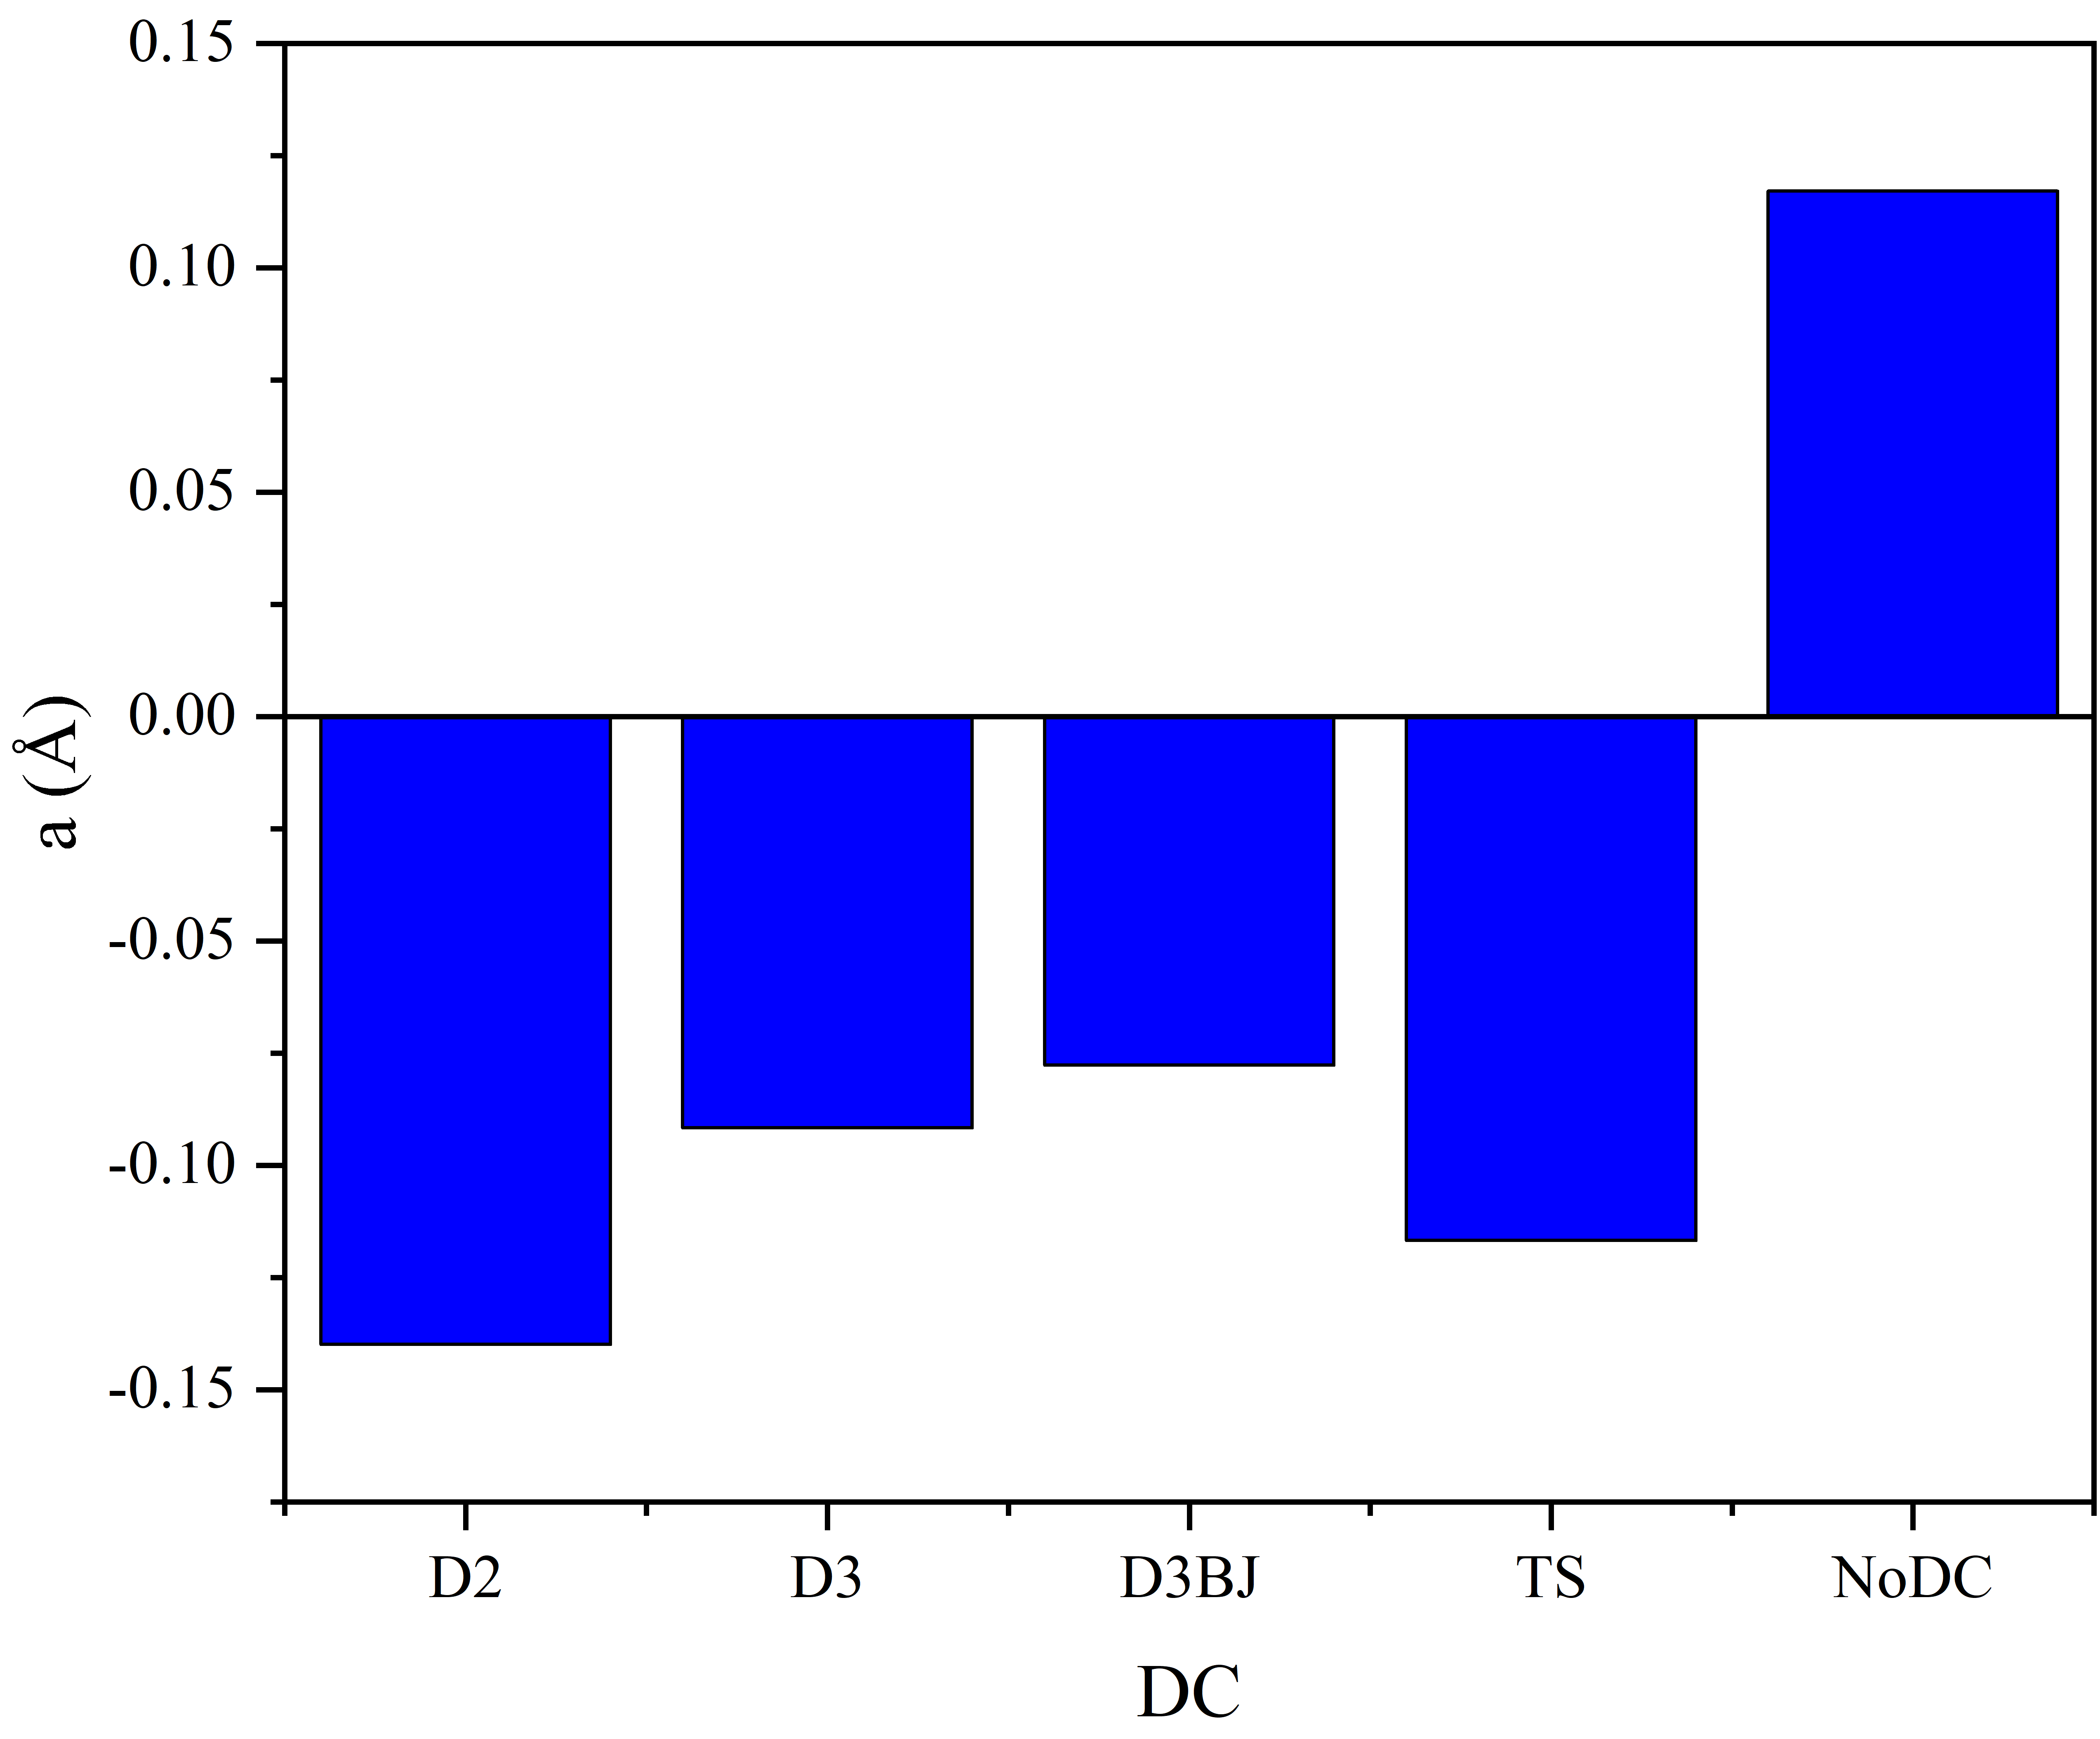
\includegraphics[width=\textwidth]{Figures/Analysis/IVDW/achnagebar.png}
\caption{a-axis of unit cell difference.}
\label{fig:StructAnal_D2}
\end{subfigure}
\begin{subfigure}{0.49\textwidth}
\centering
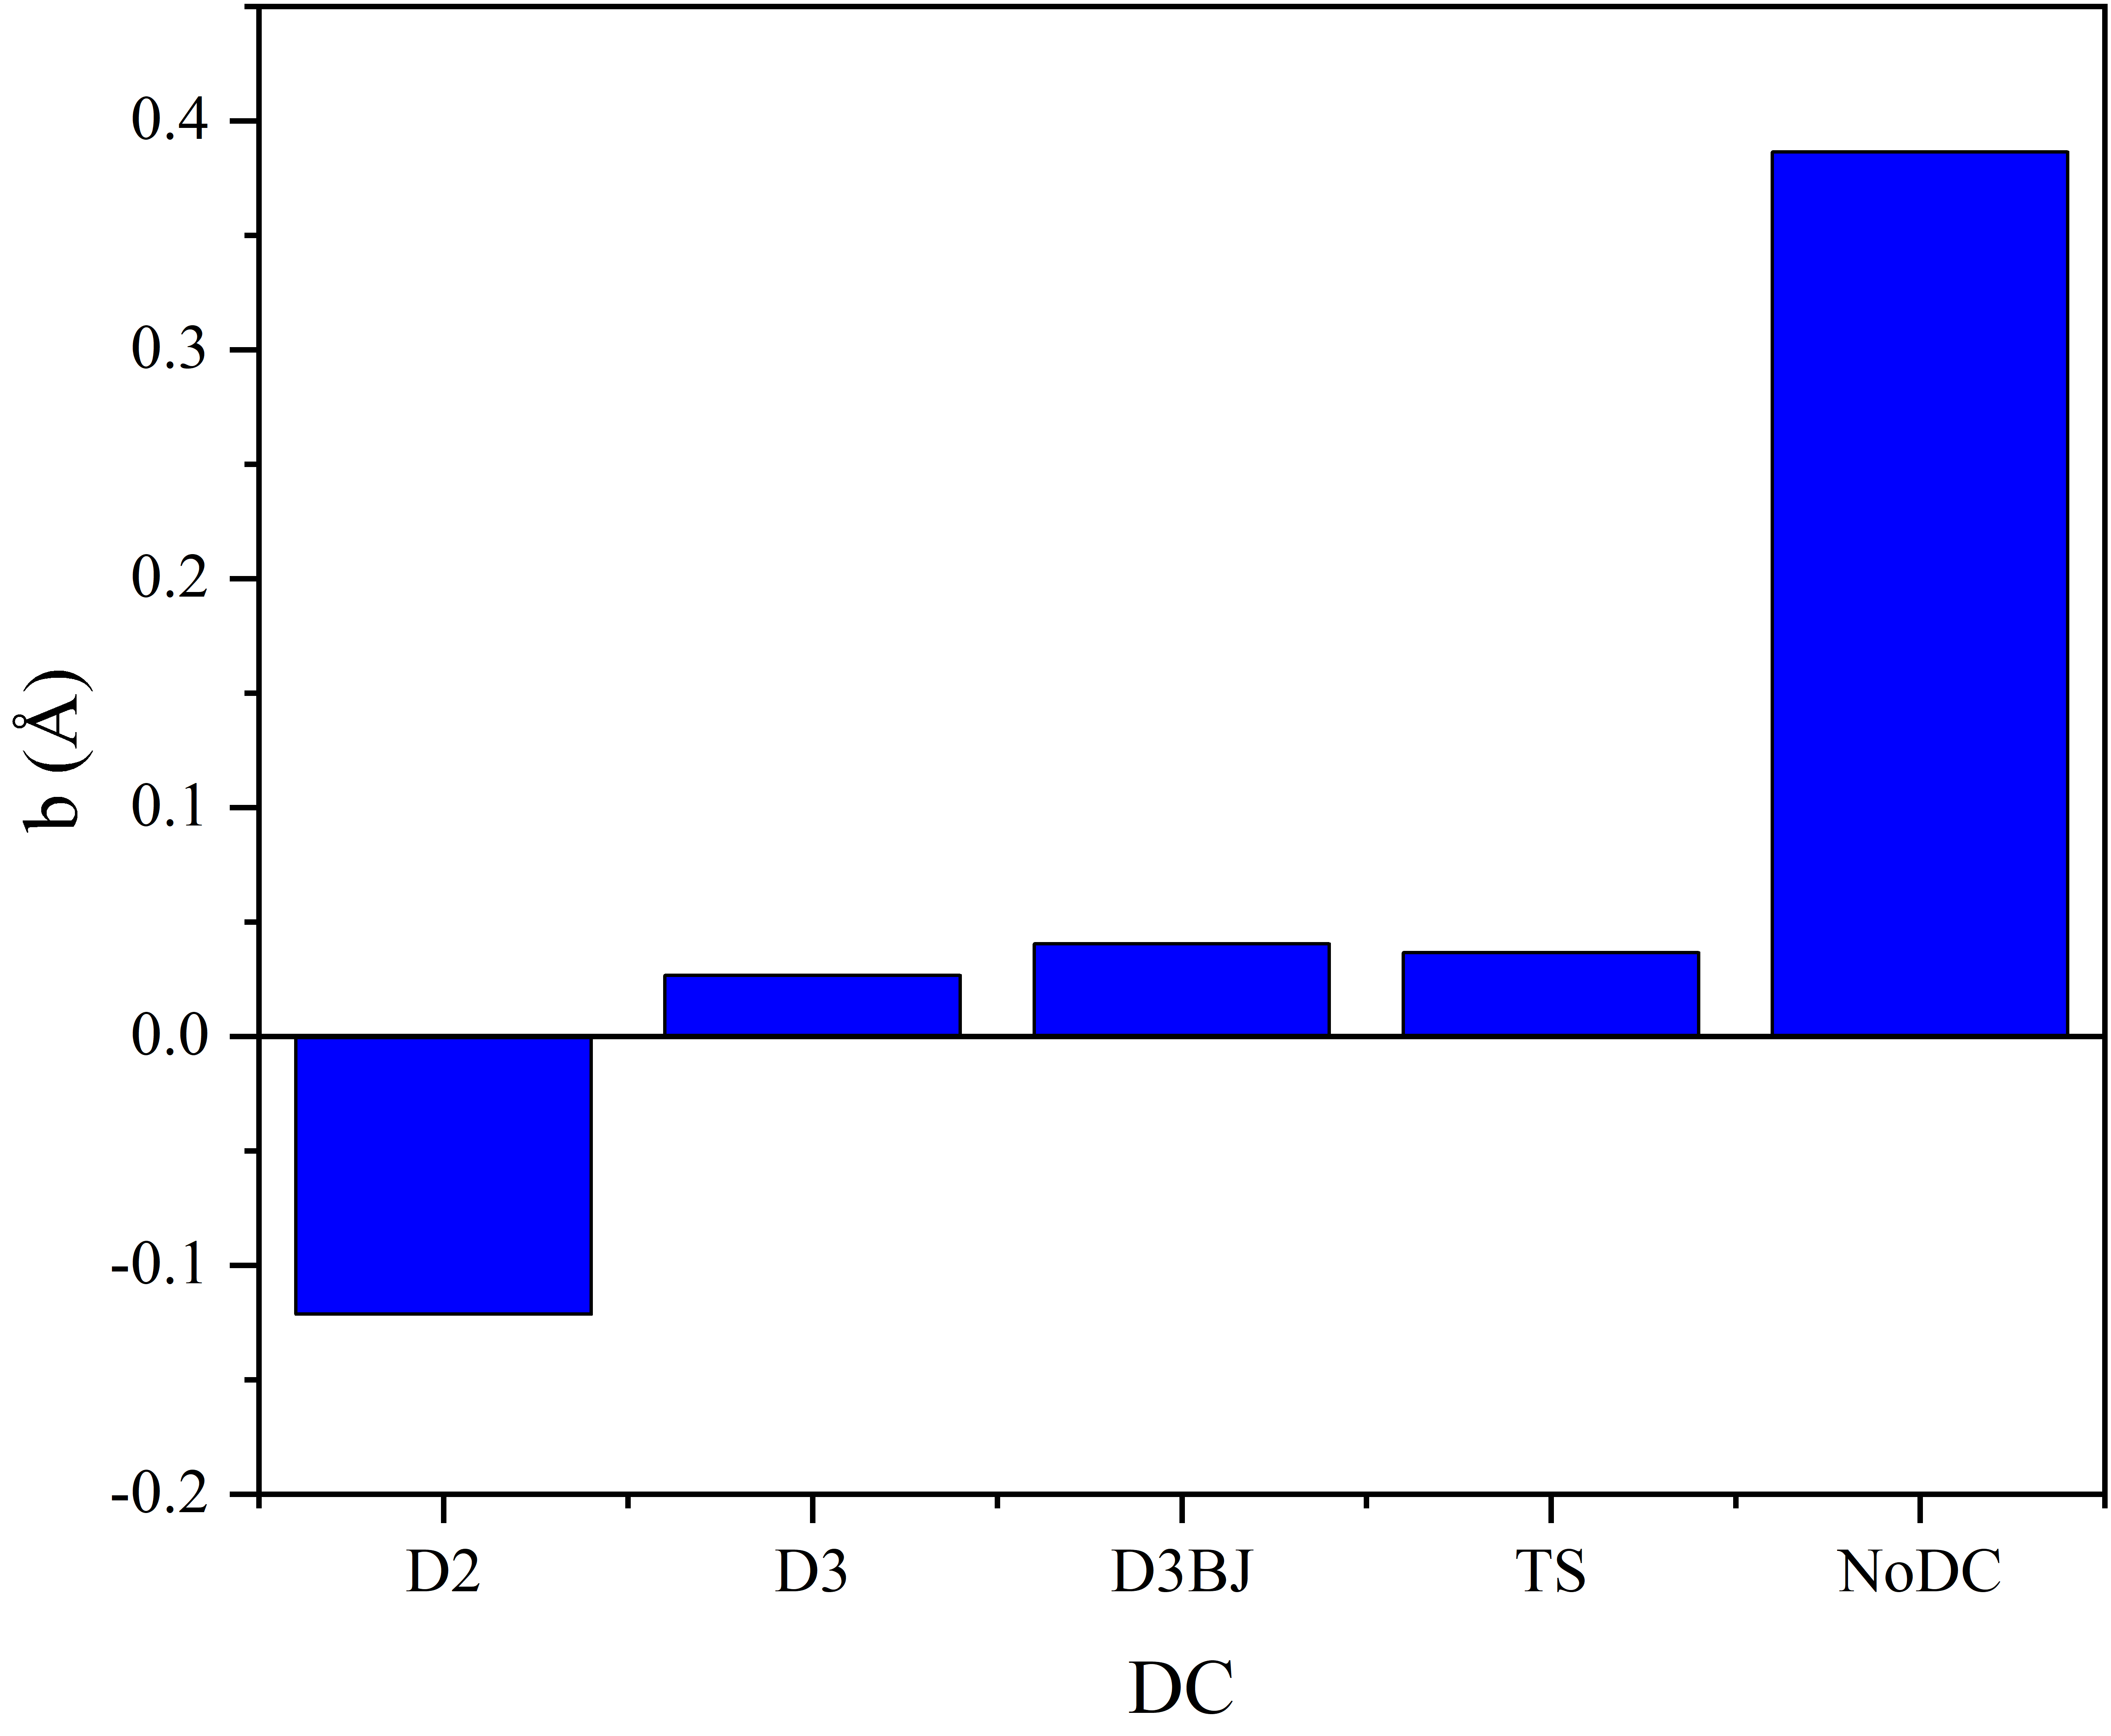
\includegraphics[width=\textwidth]{Figures/Analysis/IVDW/bchangebar.png}
\caption{b-axis of unit cell difference.}
\label{fig:StructAnal_D3}
\end{subfigure}

\begin{subfigure}{0.49\textwidth}
\centering
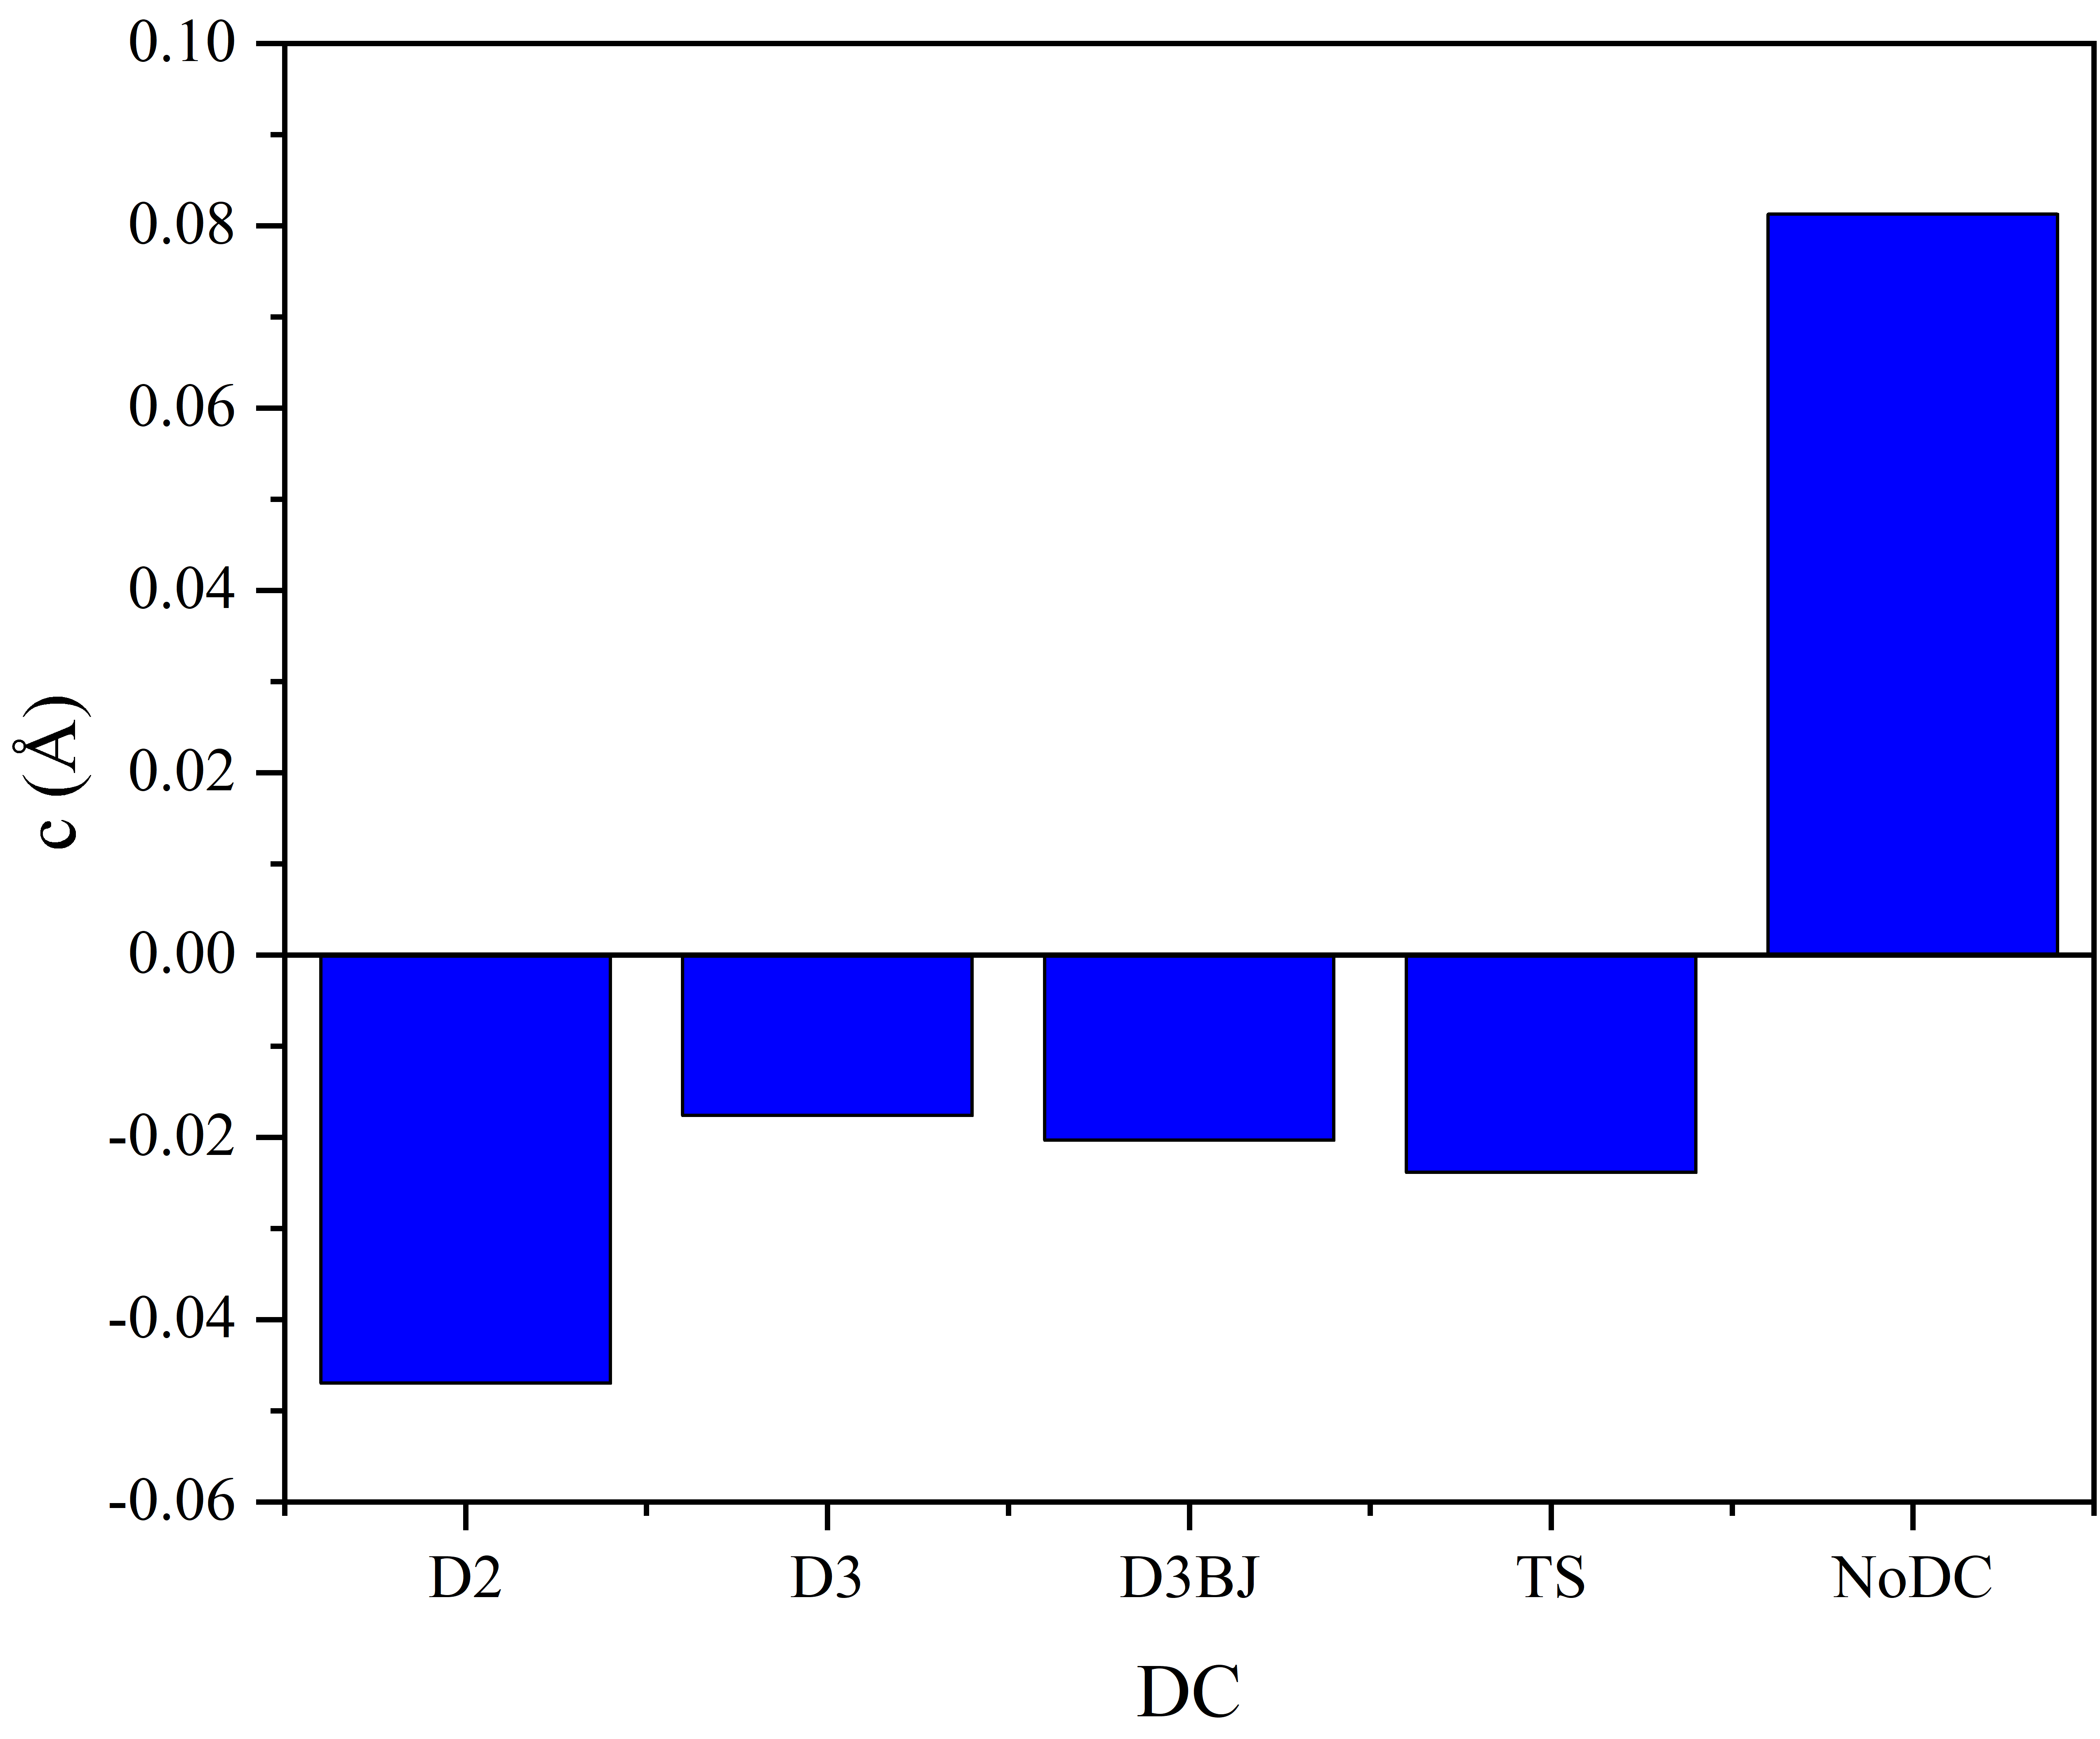
\includegraphics[width=\textwidth]{Figures/Analysis/IVDW/cchangebar.png}
\caption{c-axis of unit cell difference.}
\label{fig:StructAnal_D3BJ}
\end{subfigure}
\begin{subfigure}{0.49\textwidth}
\centering
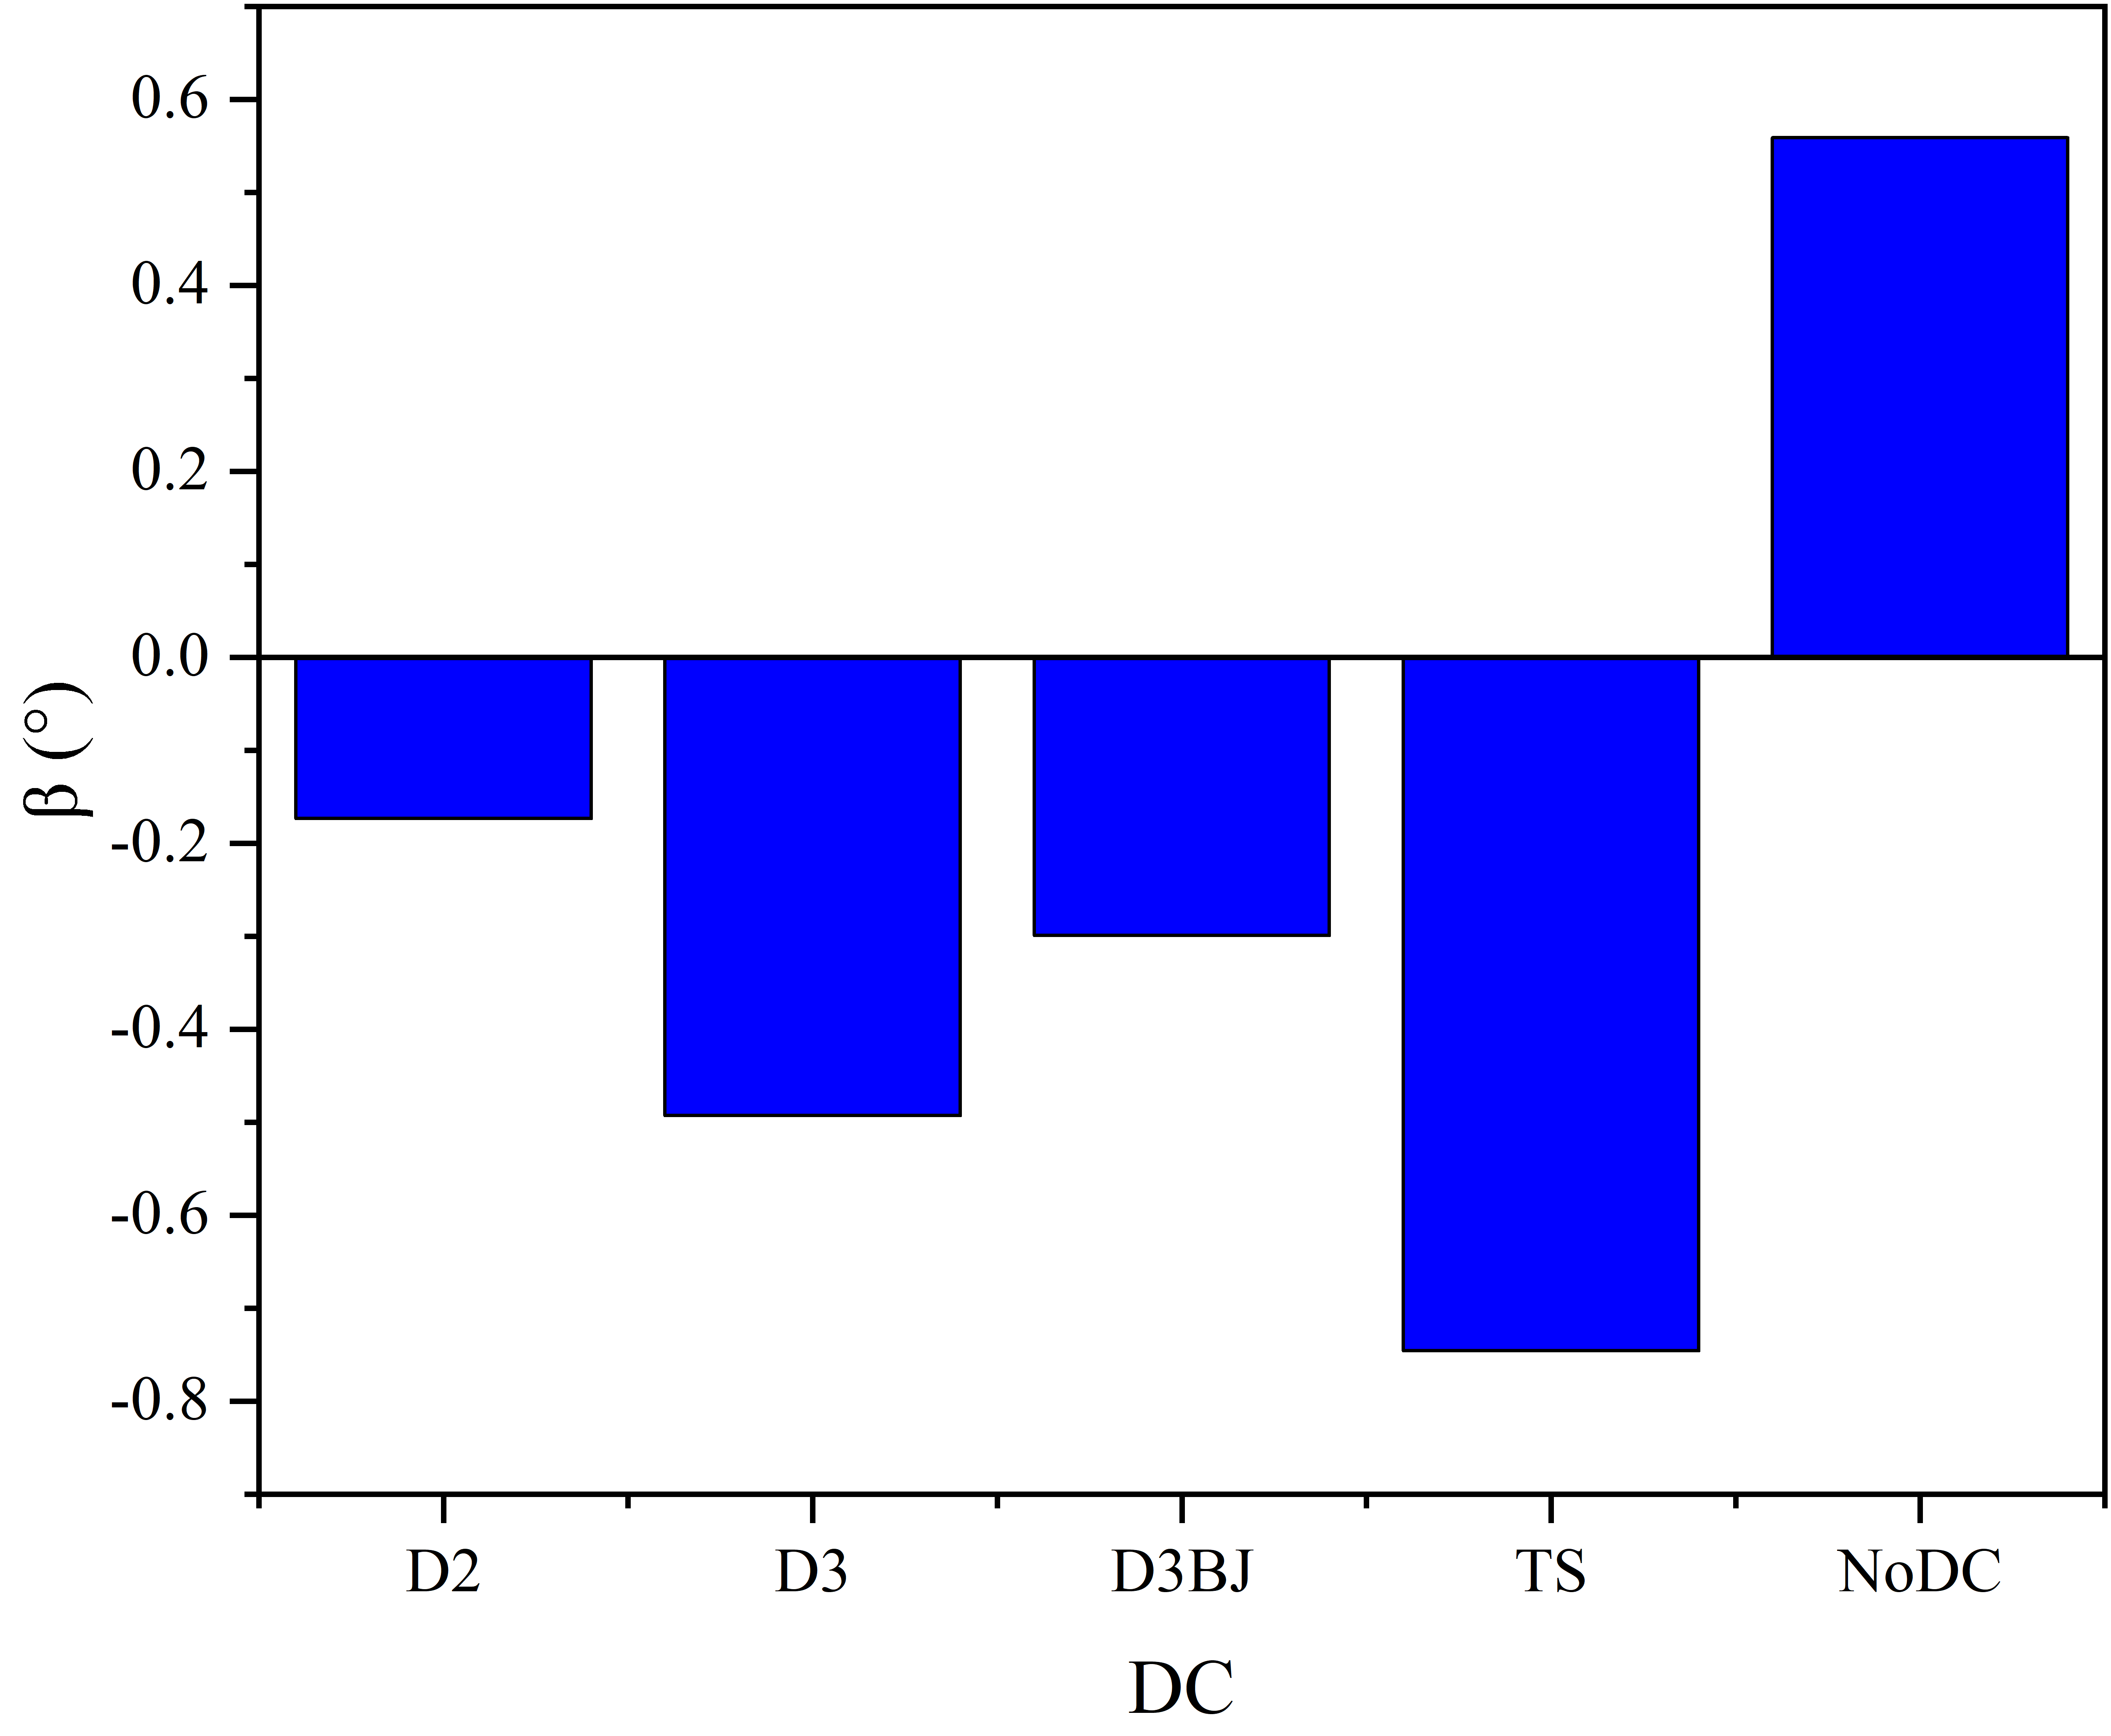
\includegraphics[width=\textwidth]{Figures/Analysis/IVDW/betachangebar.png}
\caption{\(\beta\) angle of unit cell difference.}
\label{fig:StructAnal_TS}
\end{subfigure}

\begin{subfigure}{0.49\textwidth}
\centering
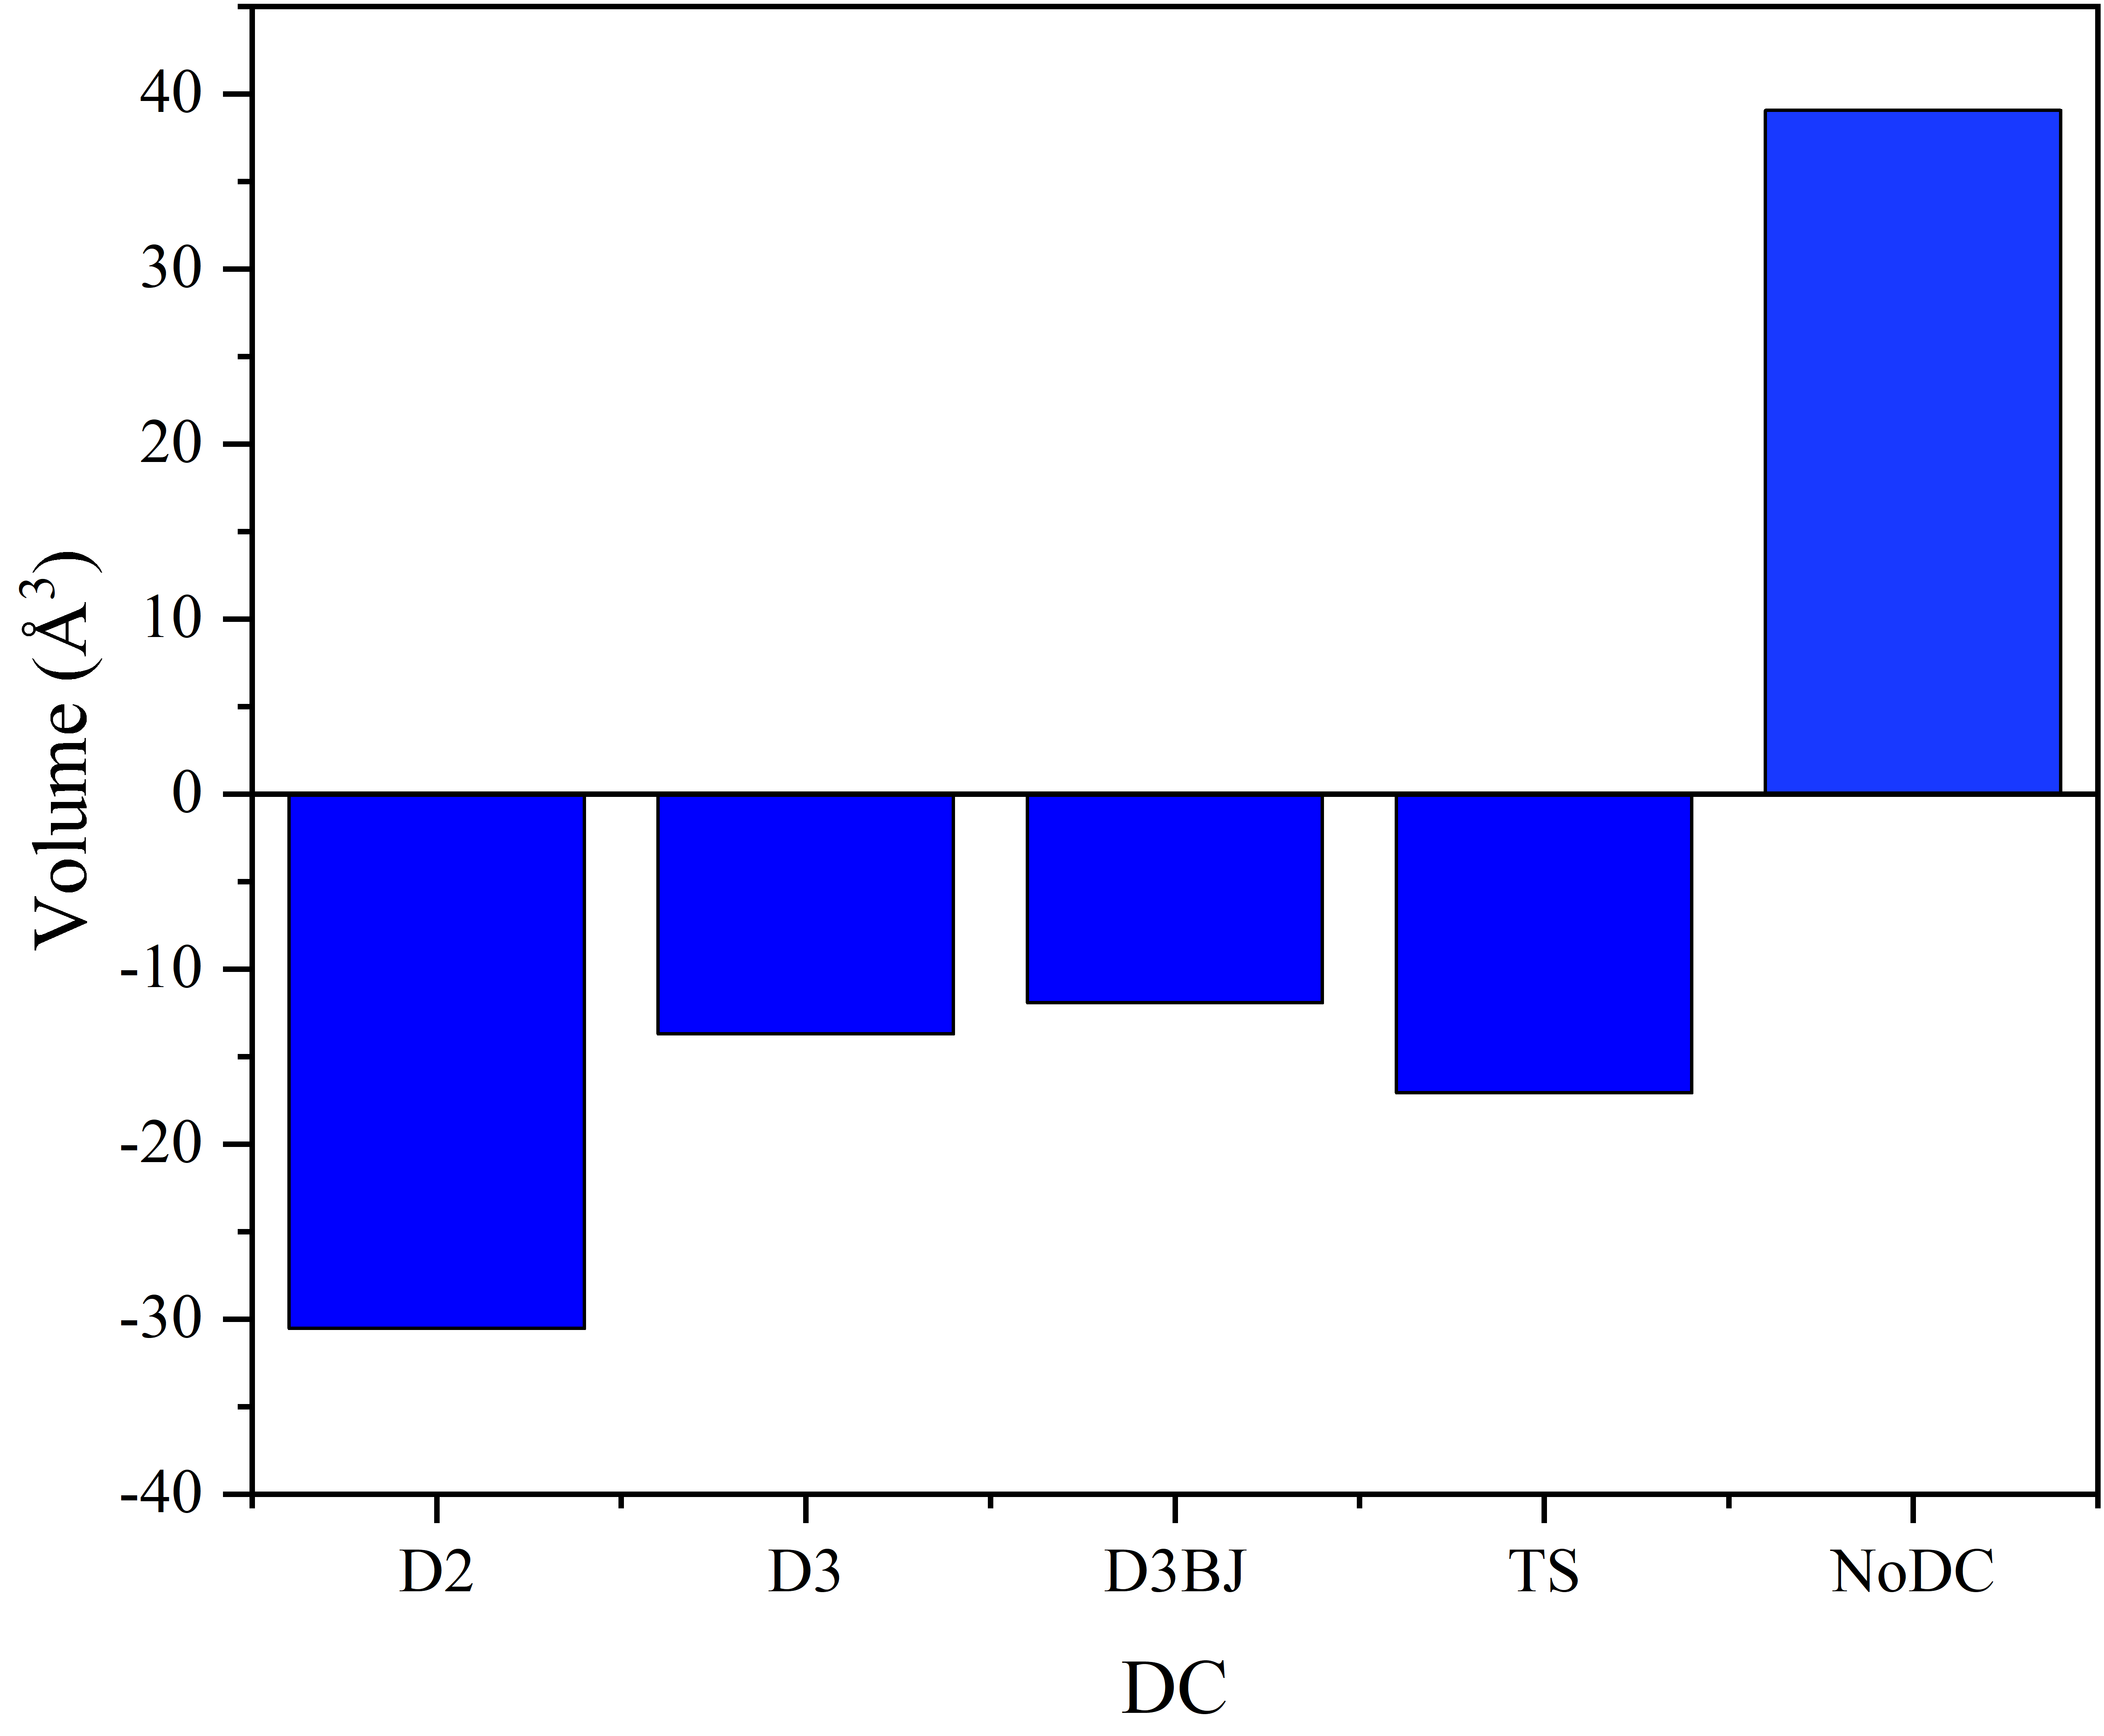
\includegraphics[width=\textwidth]{Figures/Analysis/IVDW/volchangebar.png}
\caption{Volume of unit cell difference.}
\label{fig:volchange}
\end{subfigure}

\captionsetup{font = footnotesize, justification = centering}
\caption[Differences between the Starting and Final Unit Cell Parameters]{The differences between the starting and final unit cell parameters. As expected, the volume increased for no correction and decreased too much for the D2 correction. The other corrections have had similar effects on the unit cell.\DIFdelbeginFL \DIFdelFL{The a}%DIFDELCMD < \nobreakdash%%%
\DIFdelFL{-axis corresponds to the vertical axis, while the b}%DIFDELCMD < \nobreakdash%%%
\DIFdelFL{-axis corresponds to the long horizontal axis and the c}%DIFDELCMD < \nobreakdash%%%
\DIFdelFL{-axis corresponds to the short horizontal axis.}\DIFdelendFL }
\label{Fig:UnitCellParams}
\end{figure}

To ensure that no drastic change had occurred in the structures and to compare the effect of the \acrshort{dc} on the structure, some comparisons between the starting and final structures were made. As the starting structure for each optimisation was obtained at \SI{150}{K}, the optimisation should have ideally not altered the structure to a significant degree as it should already be reasonably close to the ground state. Firstly, Pymatgen \DIFdelbegin \DIFdel{~}\DIFdelend \cite{Ong2013} was used to represent the structure as a matrix that has been normalised by a scaling factor which is proportional to the volume and number of sites. The atomic sites are then compared directly and the average \acrshort{rms} displacement, normalised by a factor of \((V/n_{sites})^{1/3}\), and the largest \acrshort{rms} displacement are extracted for every atom in the unit cell with the exception of the H atoms. This is owing to the poor resolution of light atoms in \acrshort{xrd}, resulting in large changes in position during the optimisation that are unlikely to be chemically significant. These are tabulated in \Cref{tab:struct_similarity}. When the structures directly using these matrices, the D2 optimisation changed the structure the least whilst the \acrshort{ts} structure was changed the most, when considering both average and maximum \acrshort{rms} displacement.

\begin{table}[h]
\centering
\begin{tabular}{@{}cccccc@{}}
\toprule
Correction & Average & Maximum & Euclidean & Cosine \\
 & RMSD / {\AA} & RMSD / {\AA} & Distance / {\AA} & Similarity \\ 
 & (Non-H Atoms) & (Non-H Atoms) & (All Atoms) & (All Atoms) \\ \midrule
None &
  0.0760 &
  0.1491 &
  0.307 &
  0.9919 \\
D2 &
  0.0689 &
  0.1288 &
  0.358 &
  0.9883 \\
D3 &
 0.0806 & 
 0.1659 &
 0.354  & 
 0.9888 & \\
D3\acrshort{bj} &
  0.0759 &
  0.1572 &
  0.350 &
  0.9889 \\
TS &
  0.0858 &
  0.1734 &
  0.359 &
  0.9884 \\ \bottomrule
\end{tabular}
\captionsetup{font = footnotesize, justification = centering}
\caption[The Values for the Structural Analysis Metrics]{The values for the structural analysis metrics. The average and maximum \acrshort{rms} displacement values are measured on the structure itself, whereas the euclidean distance and the cosine similarity were measured on the fingerprint structures. The \acrshort{ts} structure appears to have changed the most from the starting structure but overall, all of the structures are relatively close to the starting structure.}
\label{tab:struct_similarity}
\end{table}

These are all small changes so reasonable confidence can be assumed in the success of the geometry optimisation owing to the low temperature of the starting structure. However, this is a somewhat crude method that does not account for atomic environment. 

A method developed by Zimmerman \DIFdelbegin \DIFdel{~}\DIFdelend \cite{Ward2018} creates a `fingerprint` for each atomic site in the structure which is a vector containing its coordination environment and oxidation state as well as its Cartesian and fractional positions. These can be compared through measuring the Euclidean distance and cosine similarity of these vectors, where structures that are identical are represented by a Euclidean distance of zero and a cosine similarity of one respectively. These are also tabulated in \Cref{tab:struct_similarity}. These show a different trend than before but considering that coordination environment has a much larger effect, this is not necessarily disagreement. It is clear that the change was very similar for each correction as the variation between these values is much smaller than for the average and maximum \acrshort{rms} displacement. This also indicates that without a correction, the optimisation has changed the structure differently than with a correction. One thing that is encouraging is that the \acrshort{dc} ‘groups’ that have similar damping corrections seem to have similar effects on the structure. 

\begin{figure}
\centering

\begin{subfigure}{0.45\textwidth}
\centering
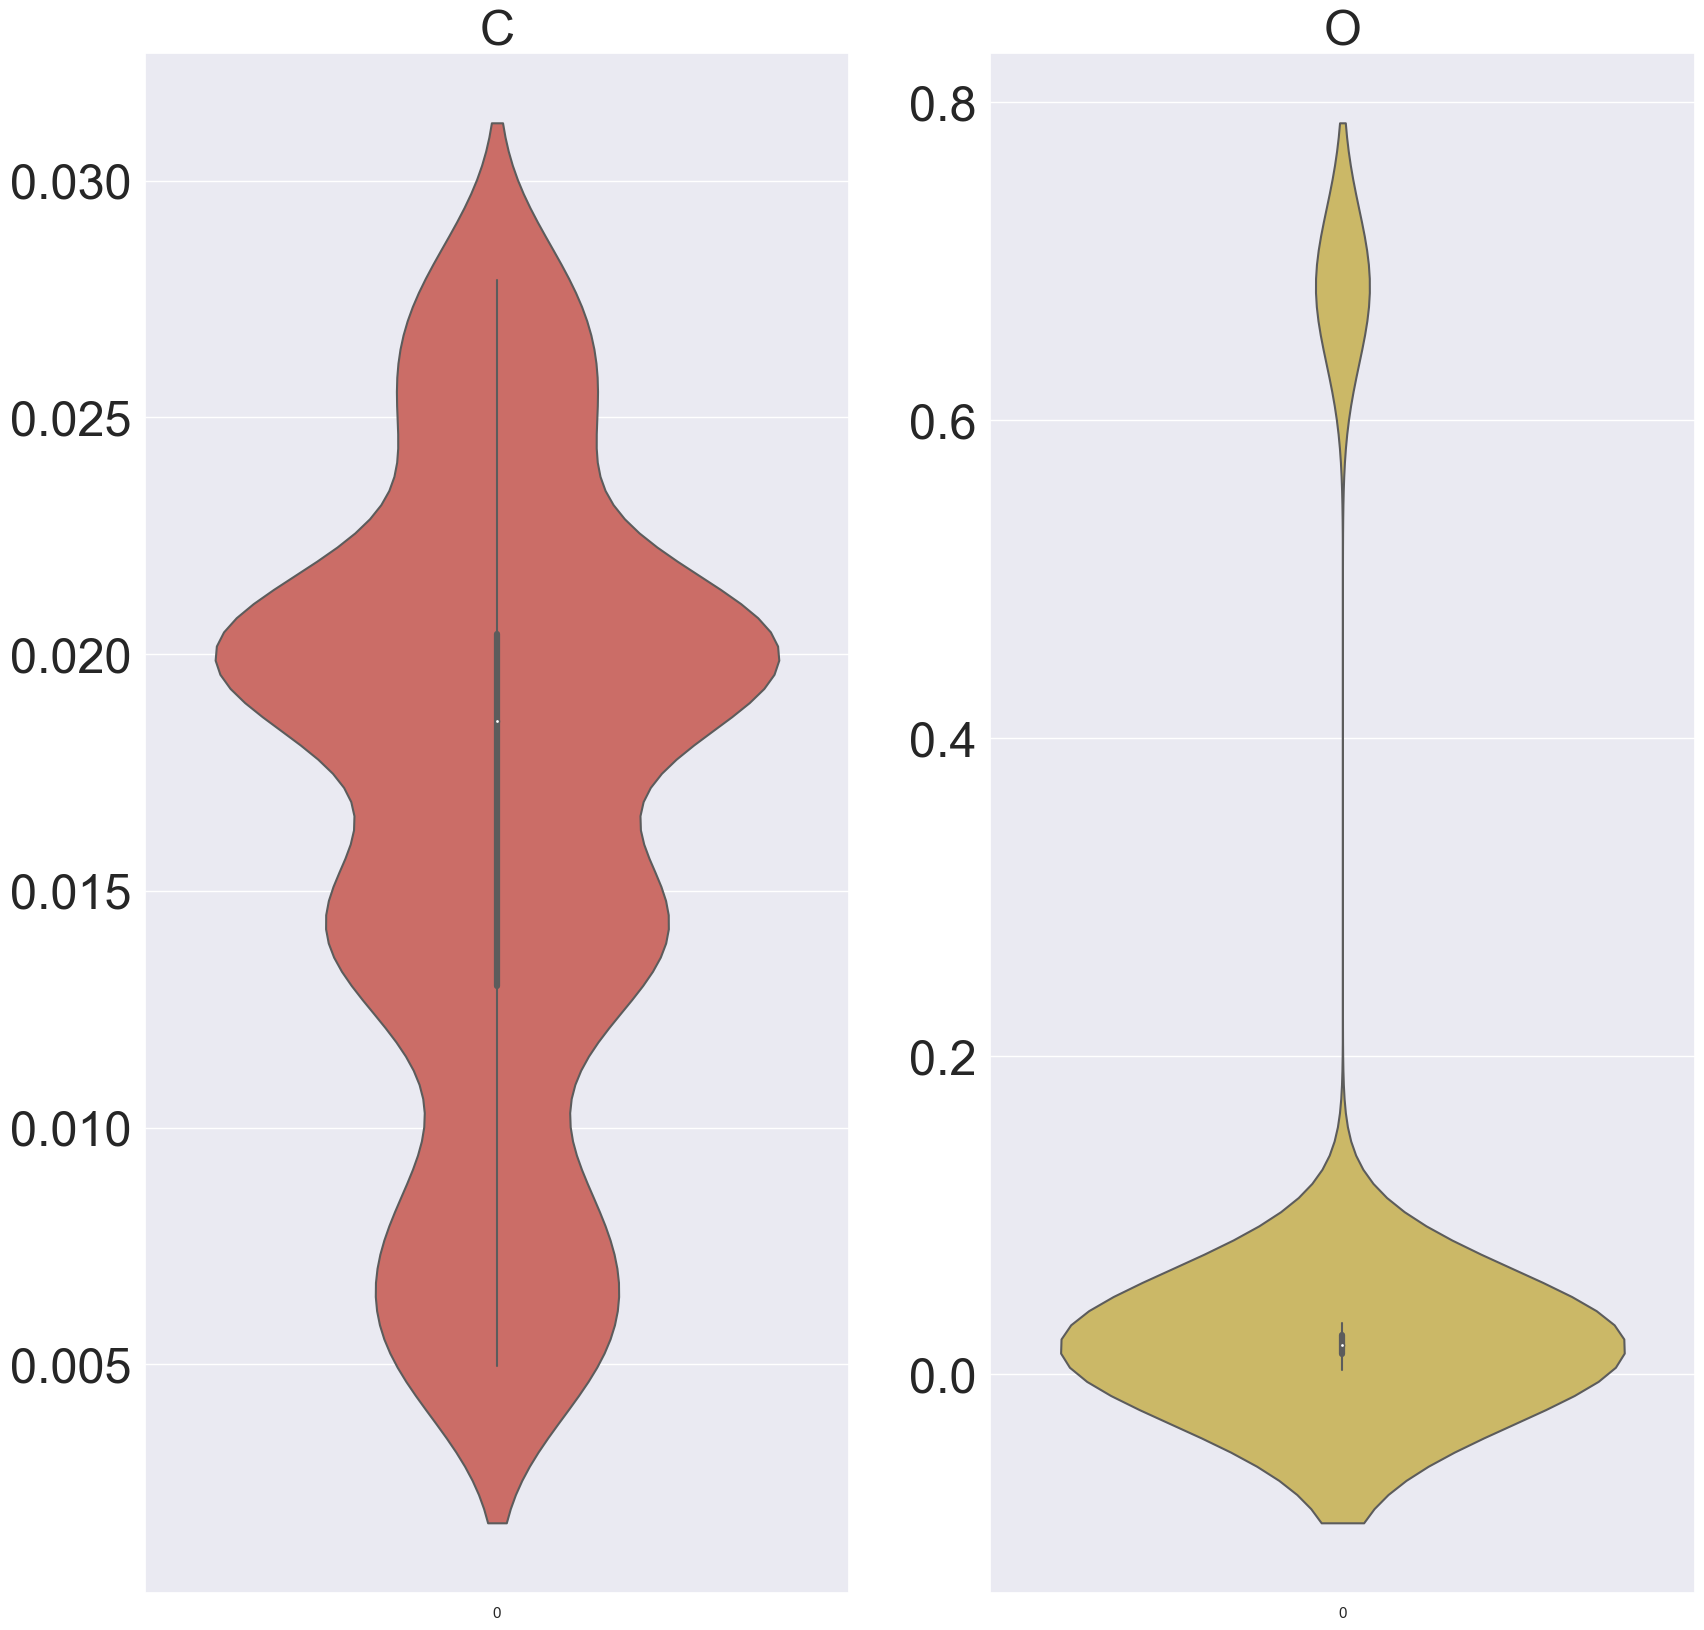
\includegraphics[width=\textwidth]{Figures/Analysis/IVDW/D2_AtomicShift_2.png}
\caption{D2}
\label{fig:StructAnal2_D2}
\end{subfigure}
\begin{subfigure}{0.45\textwidth}
\centering
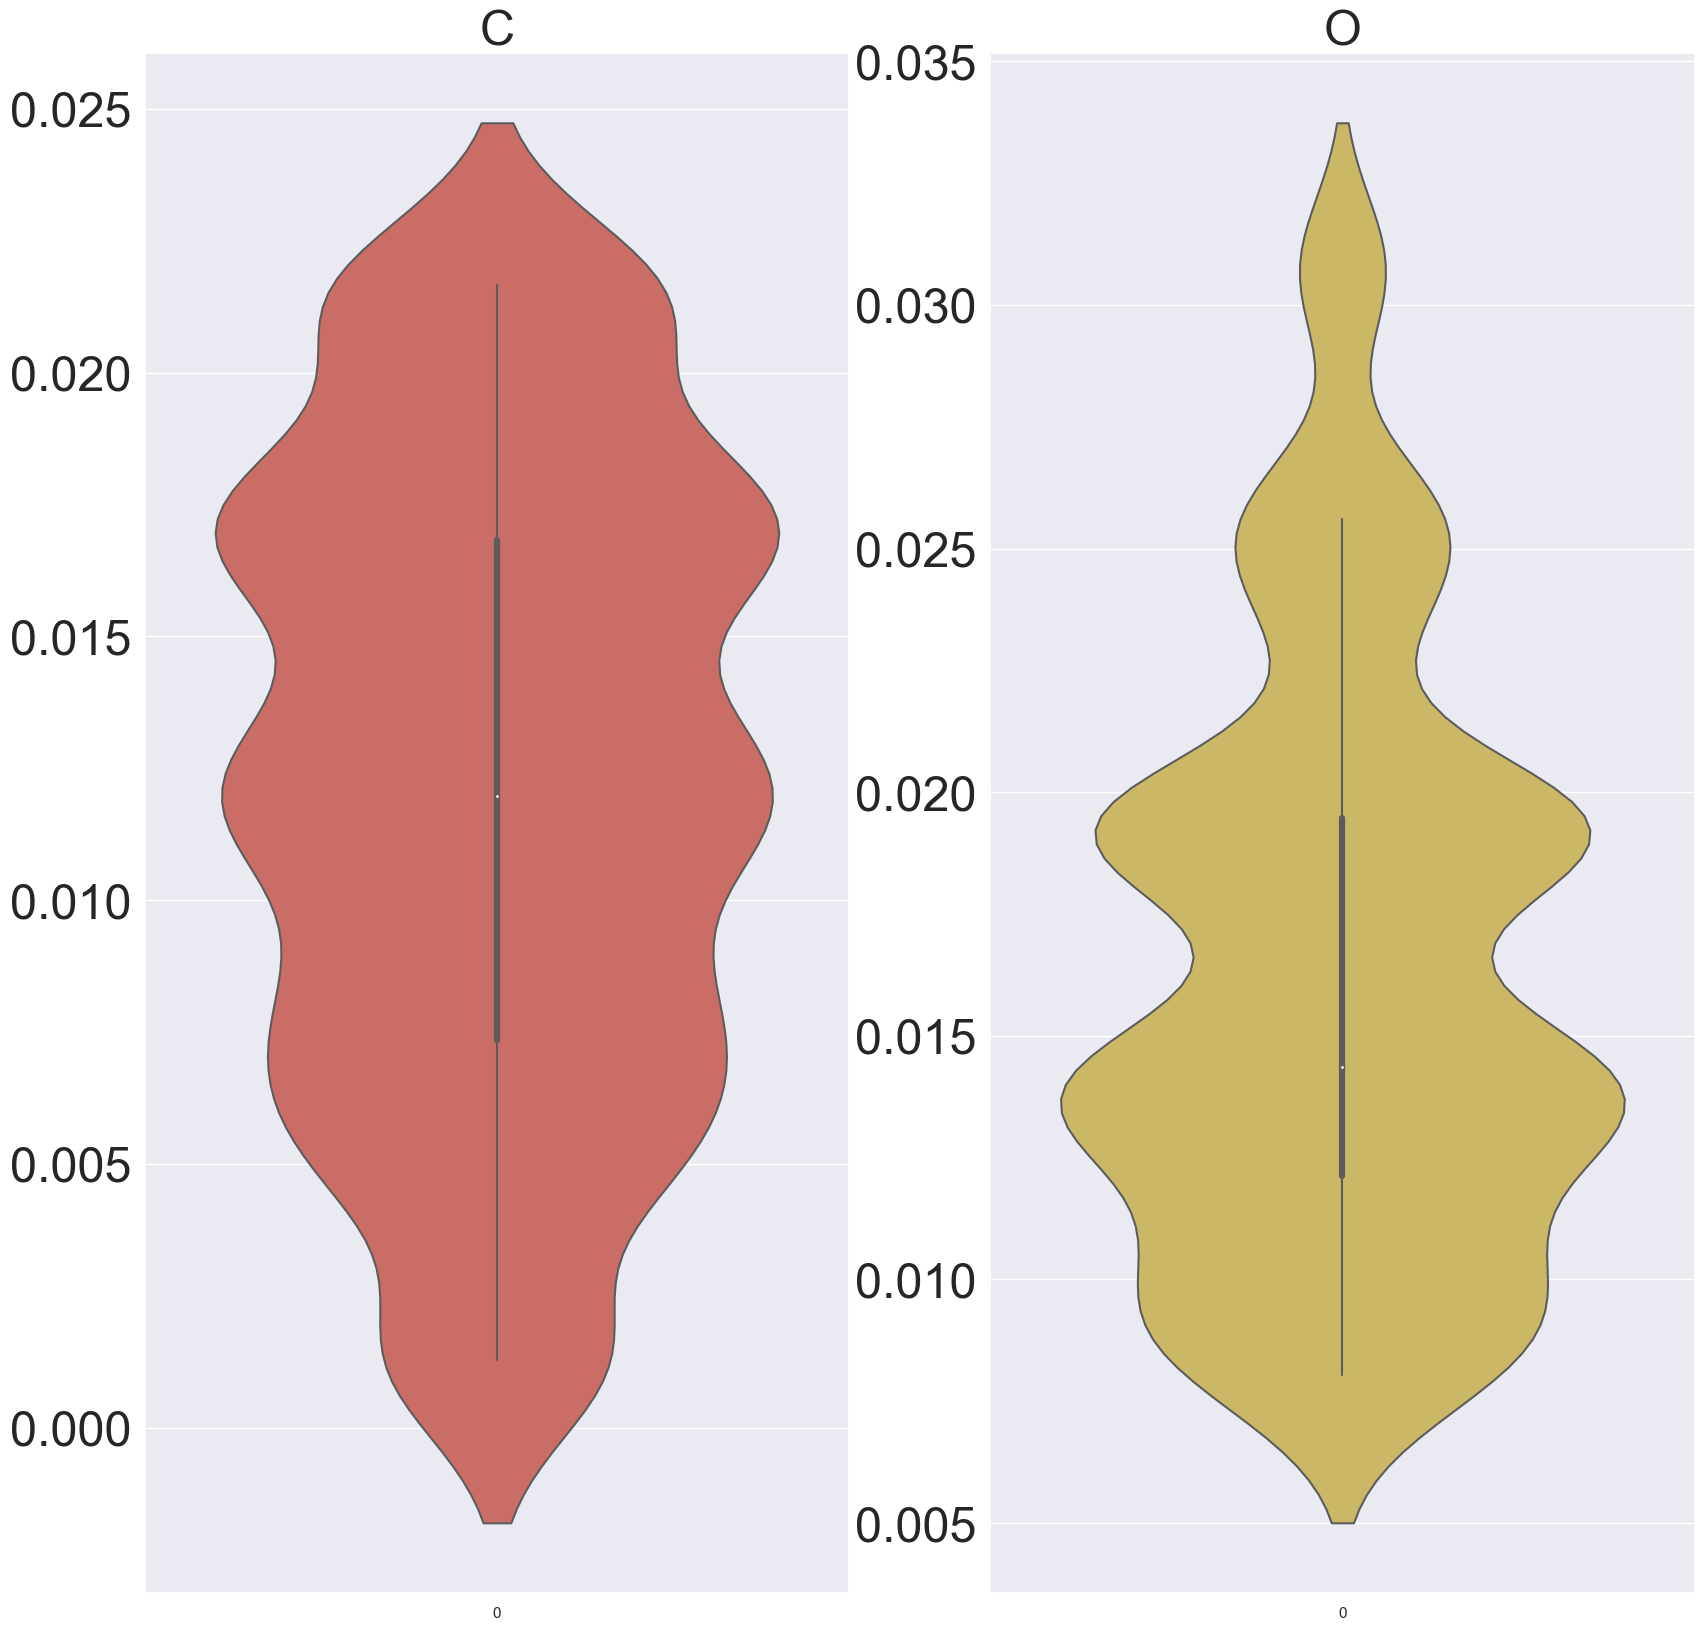
\includegraphics[width=\textwidth]{Figures/Analysis/IVDW/D3_AtomicShift_2.png}
\caption{D3}
\label{fig:StructAnal2_D3}
\end{subfigure}

\begin{subfigure}{0.45\textwidth}
\centering
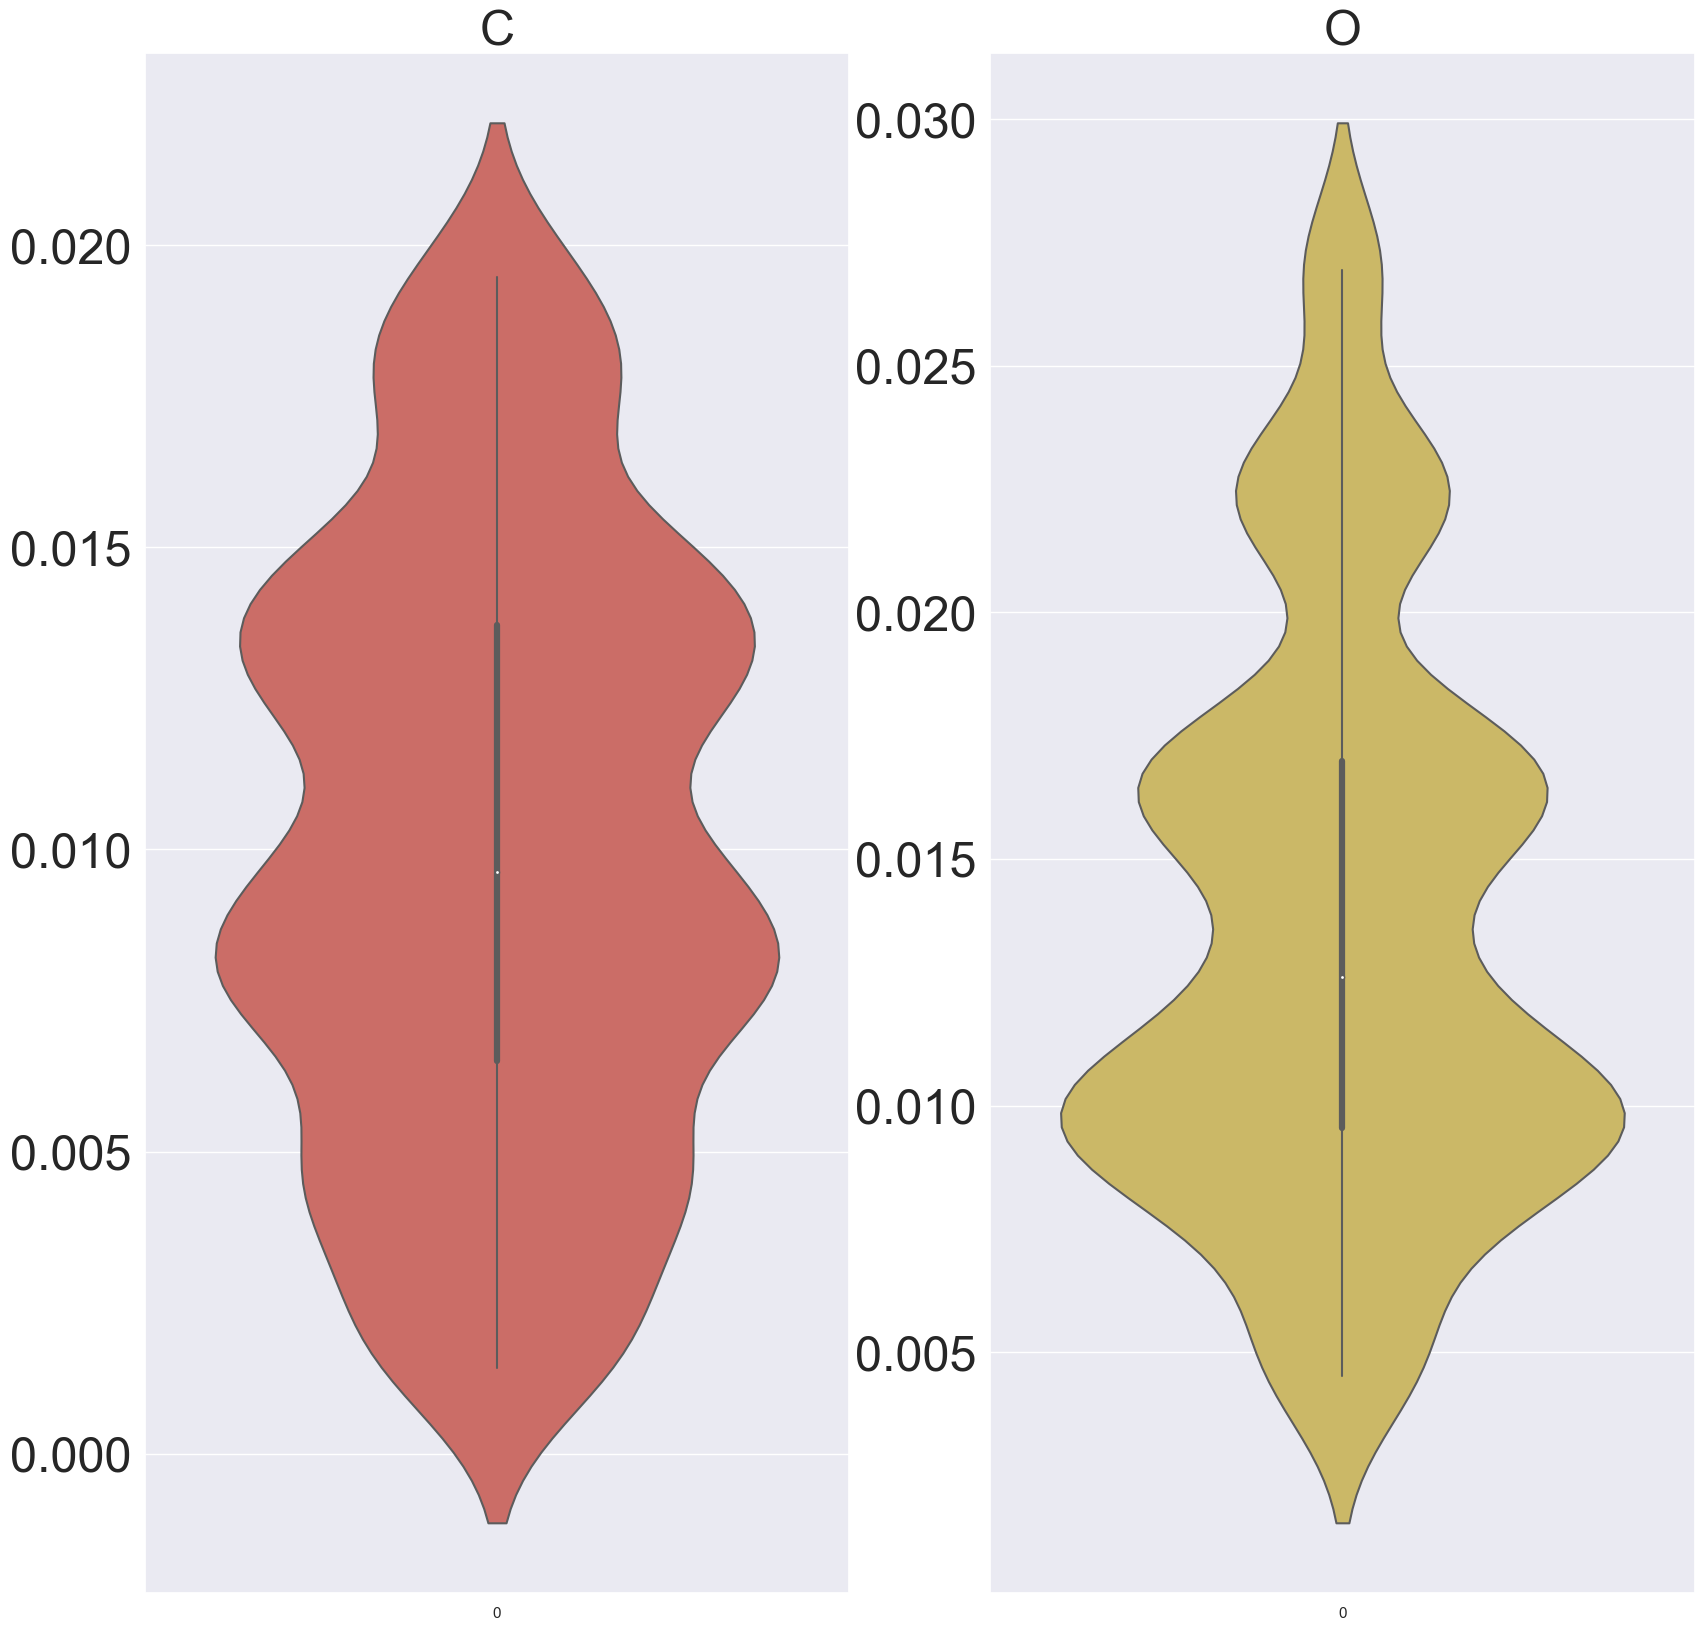
\includegraphics[width=\textwidth]{Figures/Analysis/IVDW/D3BJ_AtomicShift_2.png}
\caption{D3\acrshort{bj}}
\label{fig:StructAnal2_D3BJ}
\end{subfigure}
\begin{subfigure}{0.45\textwidth}
\centering
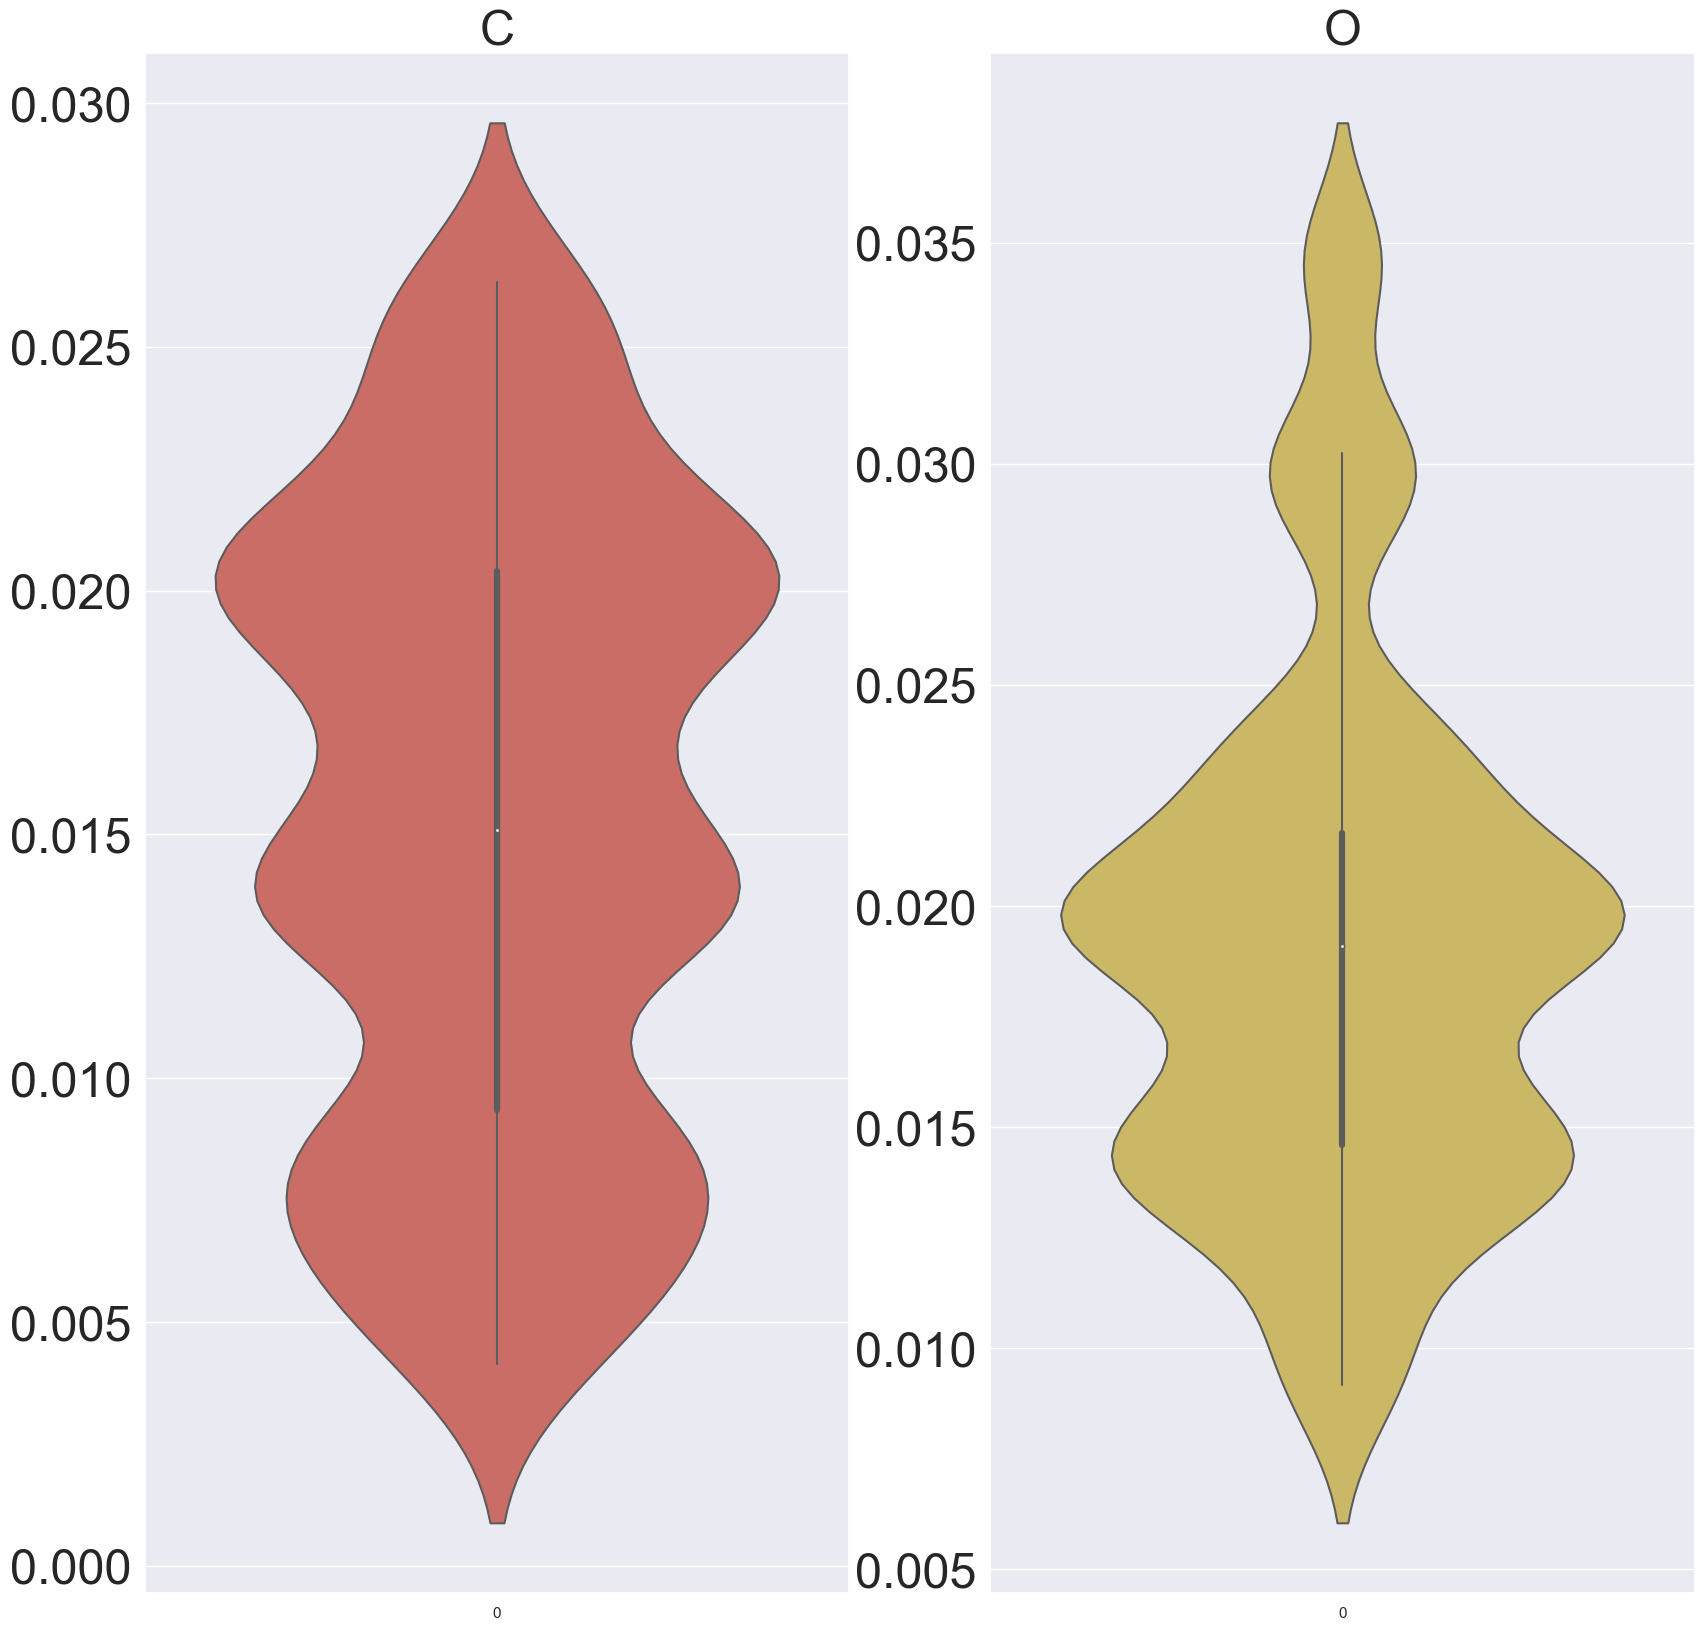
\includegraphics[width=\textwidth]{Figures/Analysis/IVDW/TS_AtomicShift_2.png}
\caption{TS}
\label{fig:StructAnal2_TS}
\end{subfigure}

\begin{subfigure}{0.45\textwidth}
\centering
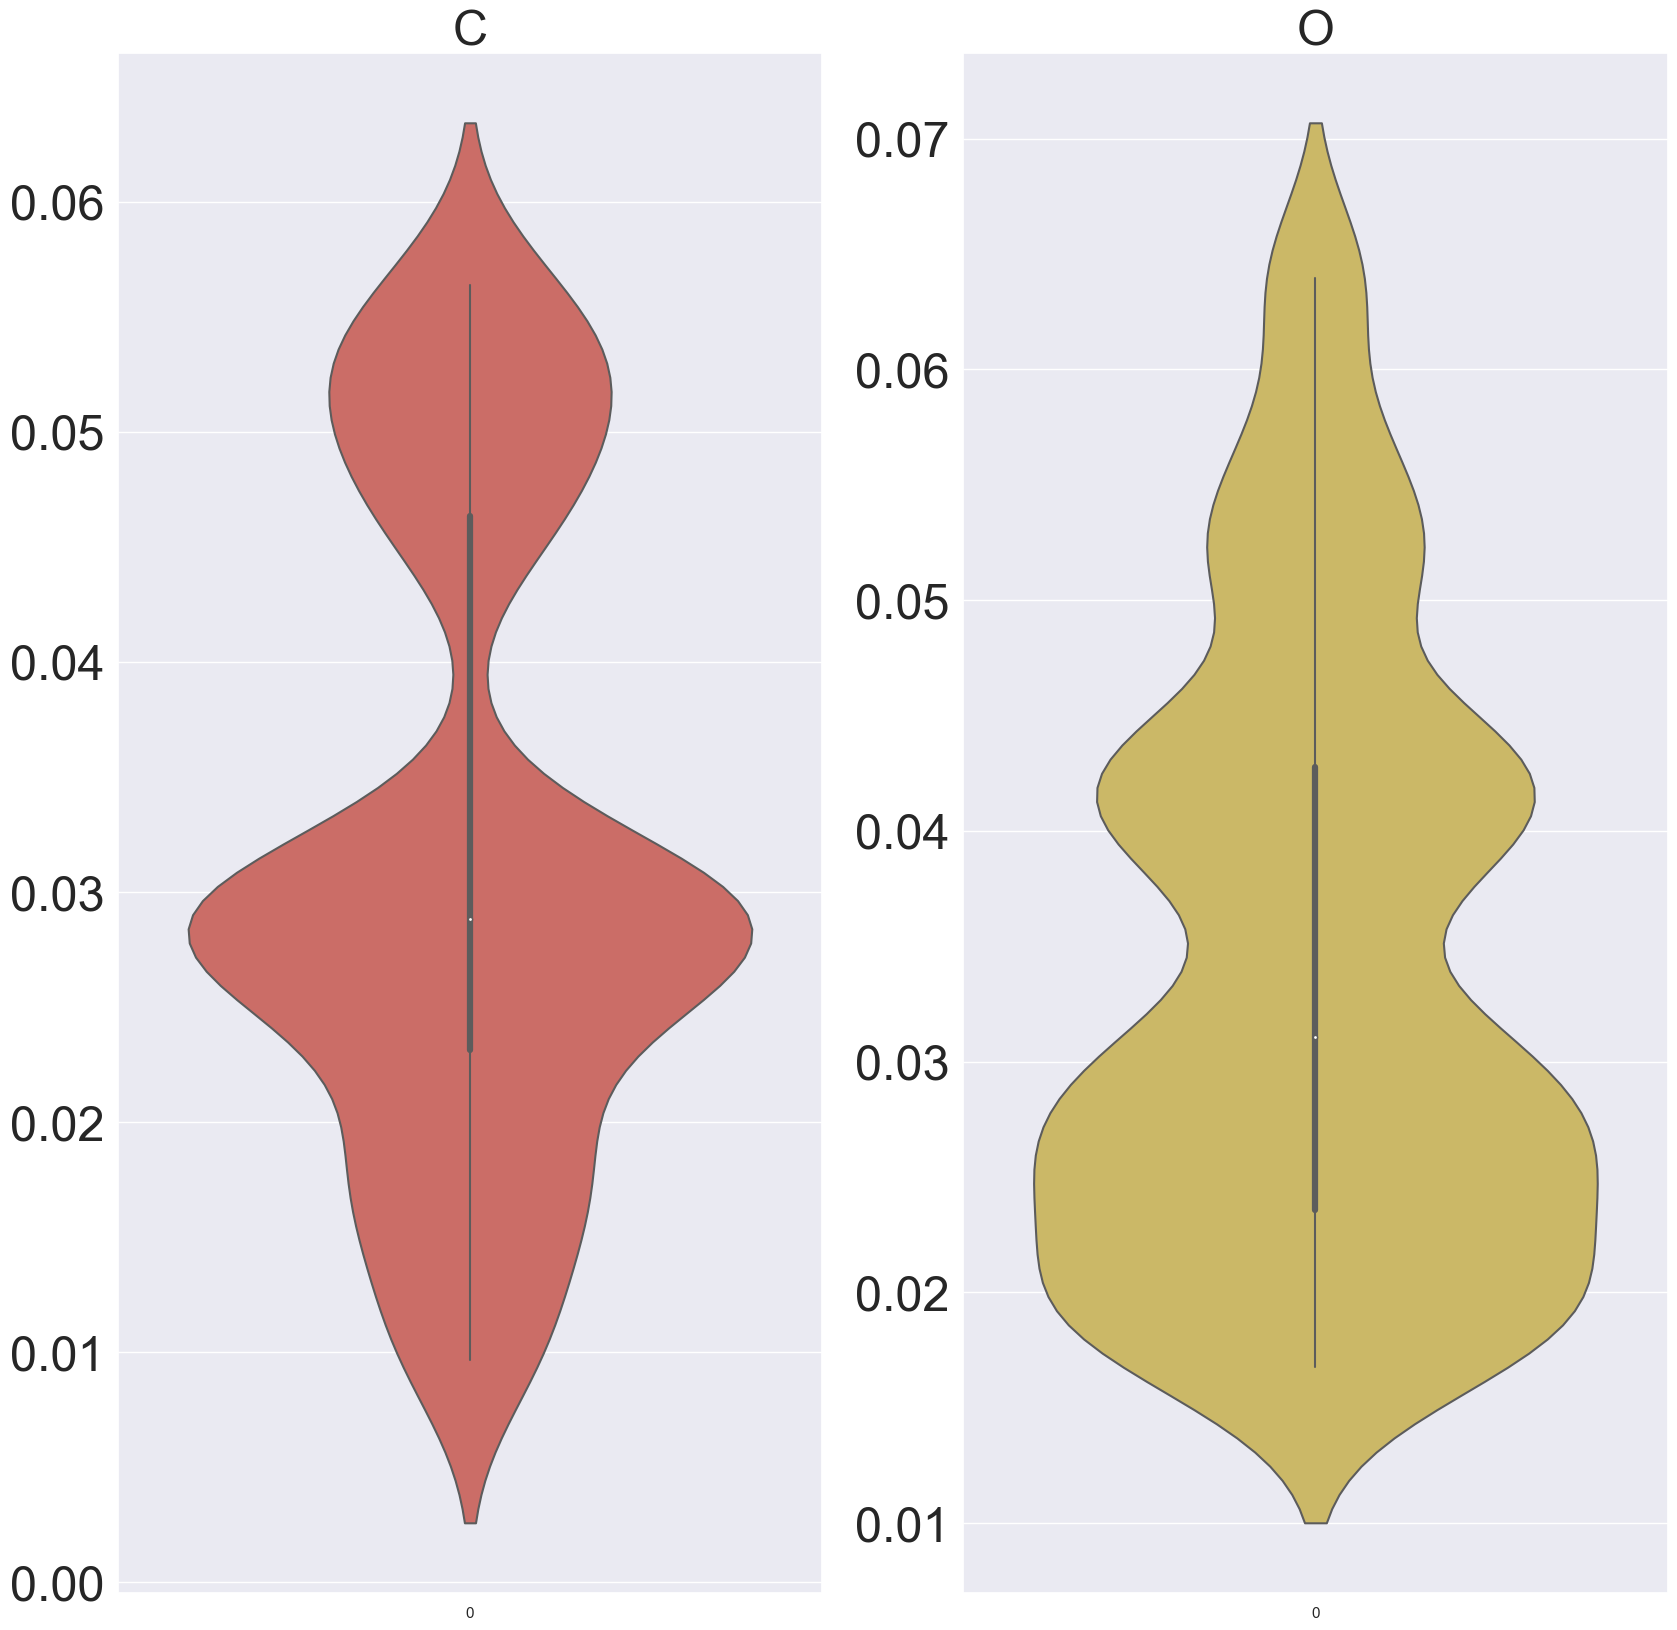
\includegraphics[width=\textwidth]{Figures/Analysis/IVDW/NoVdW_AtomicShift_2.png}
\caption{NoVdW}
\label{fig:StructAnal2_NOVDW}
\end{subfigure}
\captionsetup{font = footnotesize, justification = centering}
\DIFdelbeginFL %DIFDELCMD < \caption[The shift in ångströms of each non-H Atom for each Dispersion Correction]{%%%
\DIFdelendFL \DIFaddbeginFL \caption[The Shift of each non-H Atom for each Dispersion Correction]{\DIFaddendFL The shift of each non-H atom for each \acrshort{dc}. The D3, D3\acrshort{bj} and \acrshort{ts}corrections caused similar changes which is indicated by the shape and length of the plot. In the D2 optimisation the two O atoms that have shifted dramatically can be clearly seen. The distribution of the plot below zero does not indicate negative displacements but a large number of values close to 0. Key: C - Red; O - Yellow.}
\label{Fig:StructAnal}
\end{figure}

To understand how these small differences in structure effect the spectra, the average values do not provide enough detail. A violin plot that shows the distribution of each atom type's total shift, along with changes in bond lengths and bond angles were produced for further analysis. \Cref{Fig:StructAnal} demonstrates one of these differences where the D2 calculation has two O atoms that have moved significantly compared to the other calculations, which was the most significant shift present throughout all of the optimisations. However, analysis of the bond lengths and angles does not indicate any abnormalities so it assumed that this is owing to significant movement of the two water molecules present in the crystal structure. As above, the D2, D3 and \acrshort{ts} corrections are shown to have resulted in similar structural changes when considering the overall distribution and length of each plot. Finally, the plot for the no correction shows the C and O atoms, which make up the main backbone of the structure, moved the least of any calculation. It should be noted that whilst many of the distributions of the violin plots finish below zero, this does not indicate negative displacement. Rather, it indicates a large number of values close to zero and for an optimisation that began on a low-temperature structure, such as this one taken at \SI{150}{K}, this is a good indicator that nothing too drastic has changed. Therefore, these plots can be used as a quick test to make sure that a calculation has not changed the structure too much as well as reveal more information about the structural changes caused by the optimisation. 

\begin{figure}[h]
    \centering
    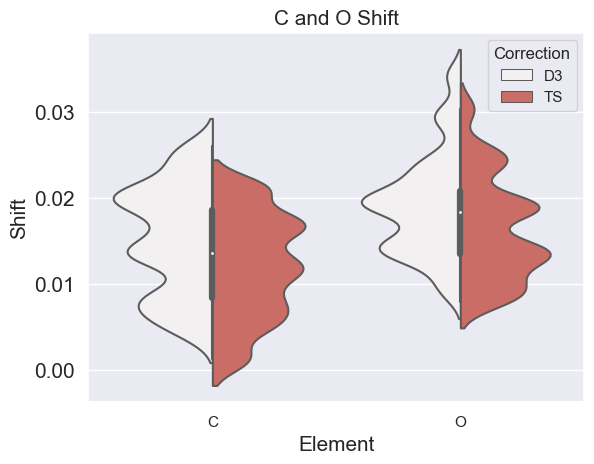
\includegraphics[width=0.7\textwidth]{Figures/Analysis/IVDW/CO_D3_TS.png}
    \captionsetup{font = footnotesize, justification = centering}
    \caption[The Direct Comparison of the Violin Plots of the D3 and TS Corrections]{The direct comparison of the violin plots of the D3 and TS corrections. It is evident that the D3 correction caused a greater shift of atomic position but that the distribution of atoms is largely similar.}
    \label{fig:TSvsD3}
\end{figure}

\Cref{fig:TSvsD3} shows the violin plots of atomic shift for the D3 and \acrshort{ts} corrections in direct comparison. It appears that the D3 correction caused the C and O atoms to shift slightly more over the course of the optimisation but that the general distribution is largely similar. This would indicate that the structures are similar in terms of relative ionic positions but appear to be shifted within the unit cell. However, these discrepancies do not appear to directly correlate to the spectral differences between the D3 and \acrshort{ts} corrections, showcased in \Cref{fig:exp_d3_ts}.

\subsection{Mode Analysis}
\label{subsec:ivdw_modeanal}
The complex variety of motion can be visually confusing for most modes when comparing calculations and so for most, visual comparison is not possible. However, for some it is and this is shown for the mode at \SI{50}{cm^{-1}} for the D2/D3 comparison in \Cref{fig:mode1_both}. Whilst the arrows are pointing in different directions, this is simply owing to them showing each half of the motion about the equilibrium position. This mode was represented well by the calculation and this seems appropriate when considering that the each molecule is moving as one entity and away from each other. These kinds of motions are probably better represented by the harmonic approximation and so match up well with experiment.

\begin{figure}[h]
\centering
\begin{subfigure}{1\textwidth}
    \centering
    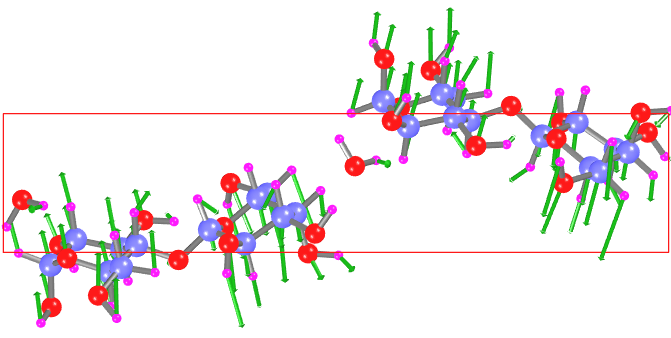
\includegraphics[scale=0.7]{Figures/Analysis/IVDW/mode8_d2_new.png}
    \caption{D2 Mode 1}
    \label{fig:d2_mode1}
\end{subfigure}
\begin{subfigure}{1\textwidth}
    \centering
    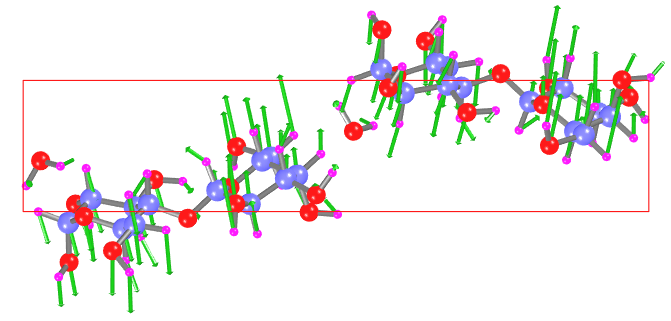
\includegraphics[scale=0.7]{Figures/Analysis/IVDW/mode8_d3_new.png}
    \caption{D3 Mode 1}
    \label{fig:d3_mode1}
\end{subfigure}
\captionsetup{font = footnotesize, justification = centering}
\caption[Mode 8 from the D2 and D3 Correction Calculations]{Mode 8 from the D2 and D3 correction calculations. This is to show that the mode orders have not changed around and mode motions are very similar. The opposing arrows between corrections is each side of the mode's motion from equilibrium.}
\label{fig:mode1_both}
\end{figure}

\begin{figure}{H}
\centering
\begin{subfigure}{0.7\textwidth}
    \centering
    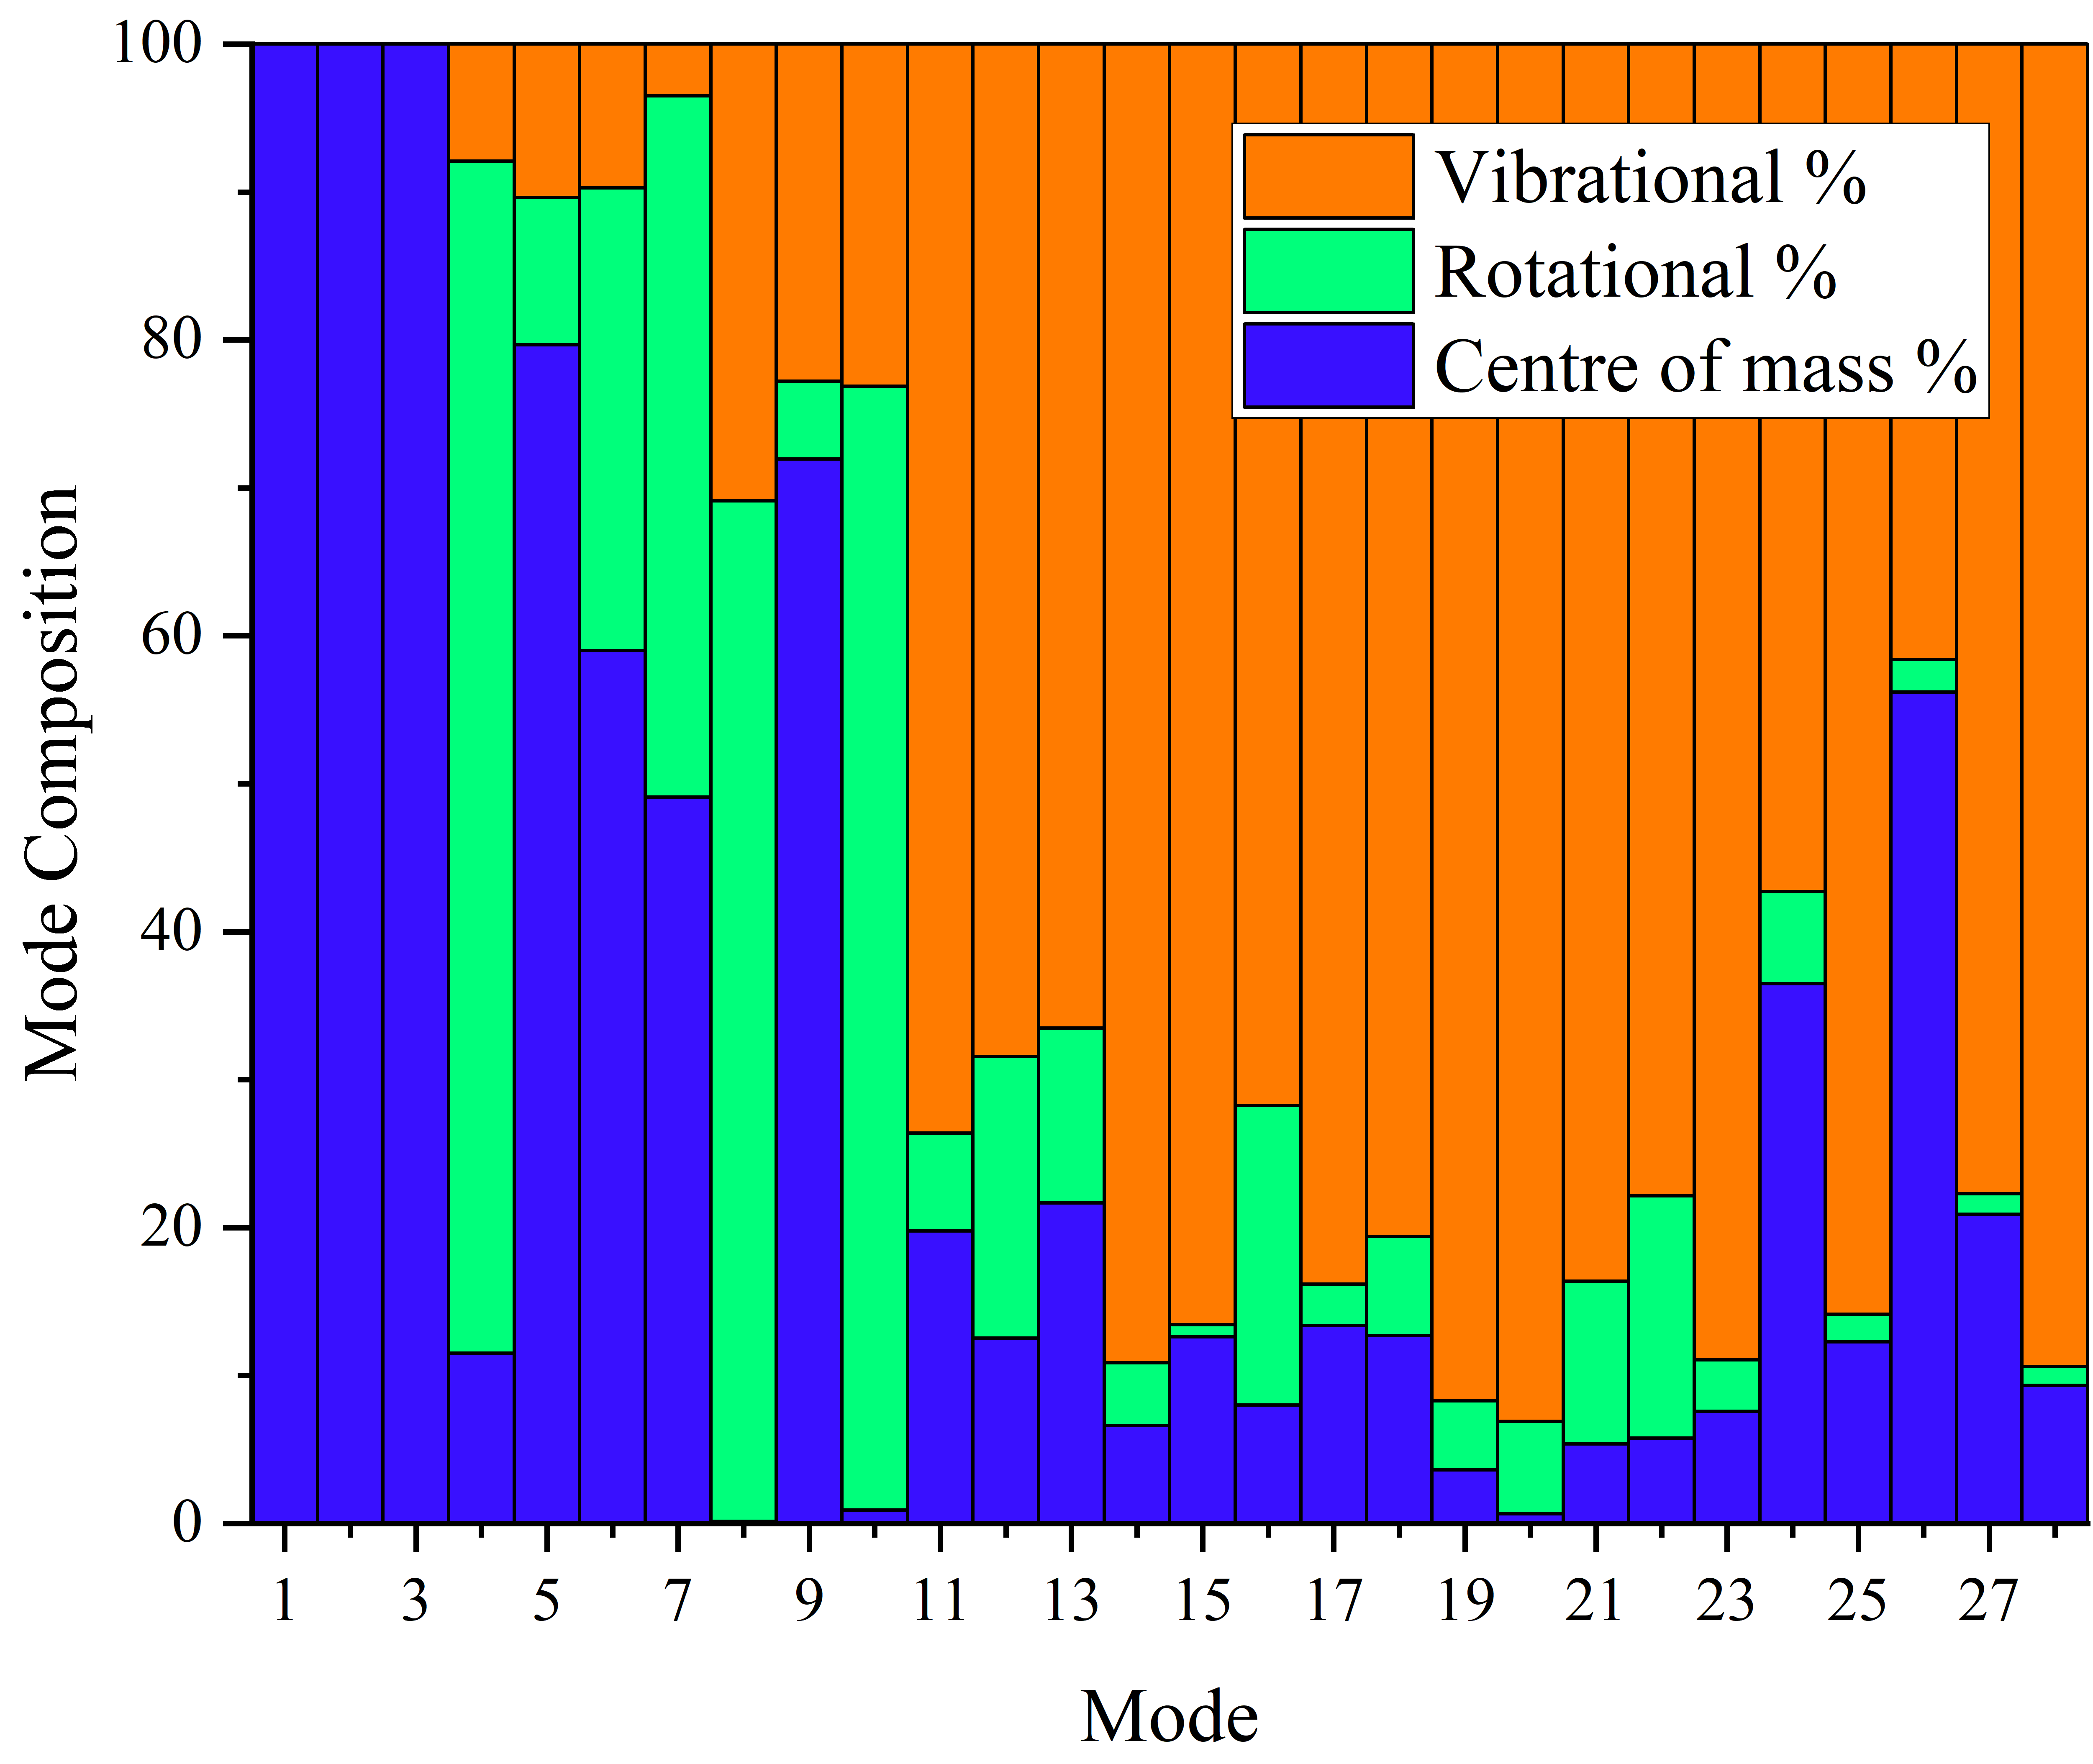
\includegraphics[scale=0.5]{Figures/Analysis/IVDW/D2ModeAnalG.png}
    \caption{D2 Mode Analysis}
    \label{fig:d2_mode_anal}
\end{subfigure}
\begin{subfigure}{1\textwidth}
    \centering
    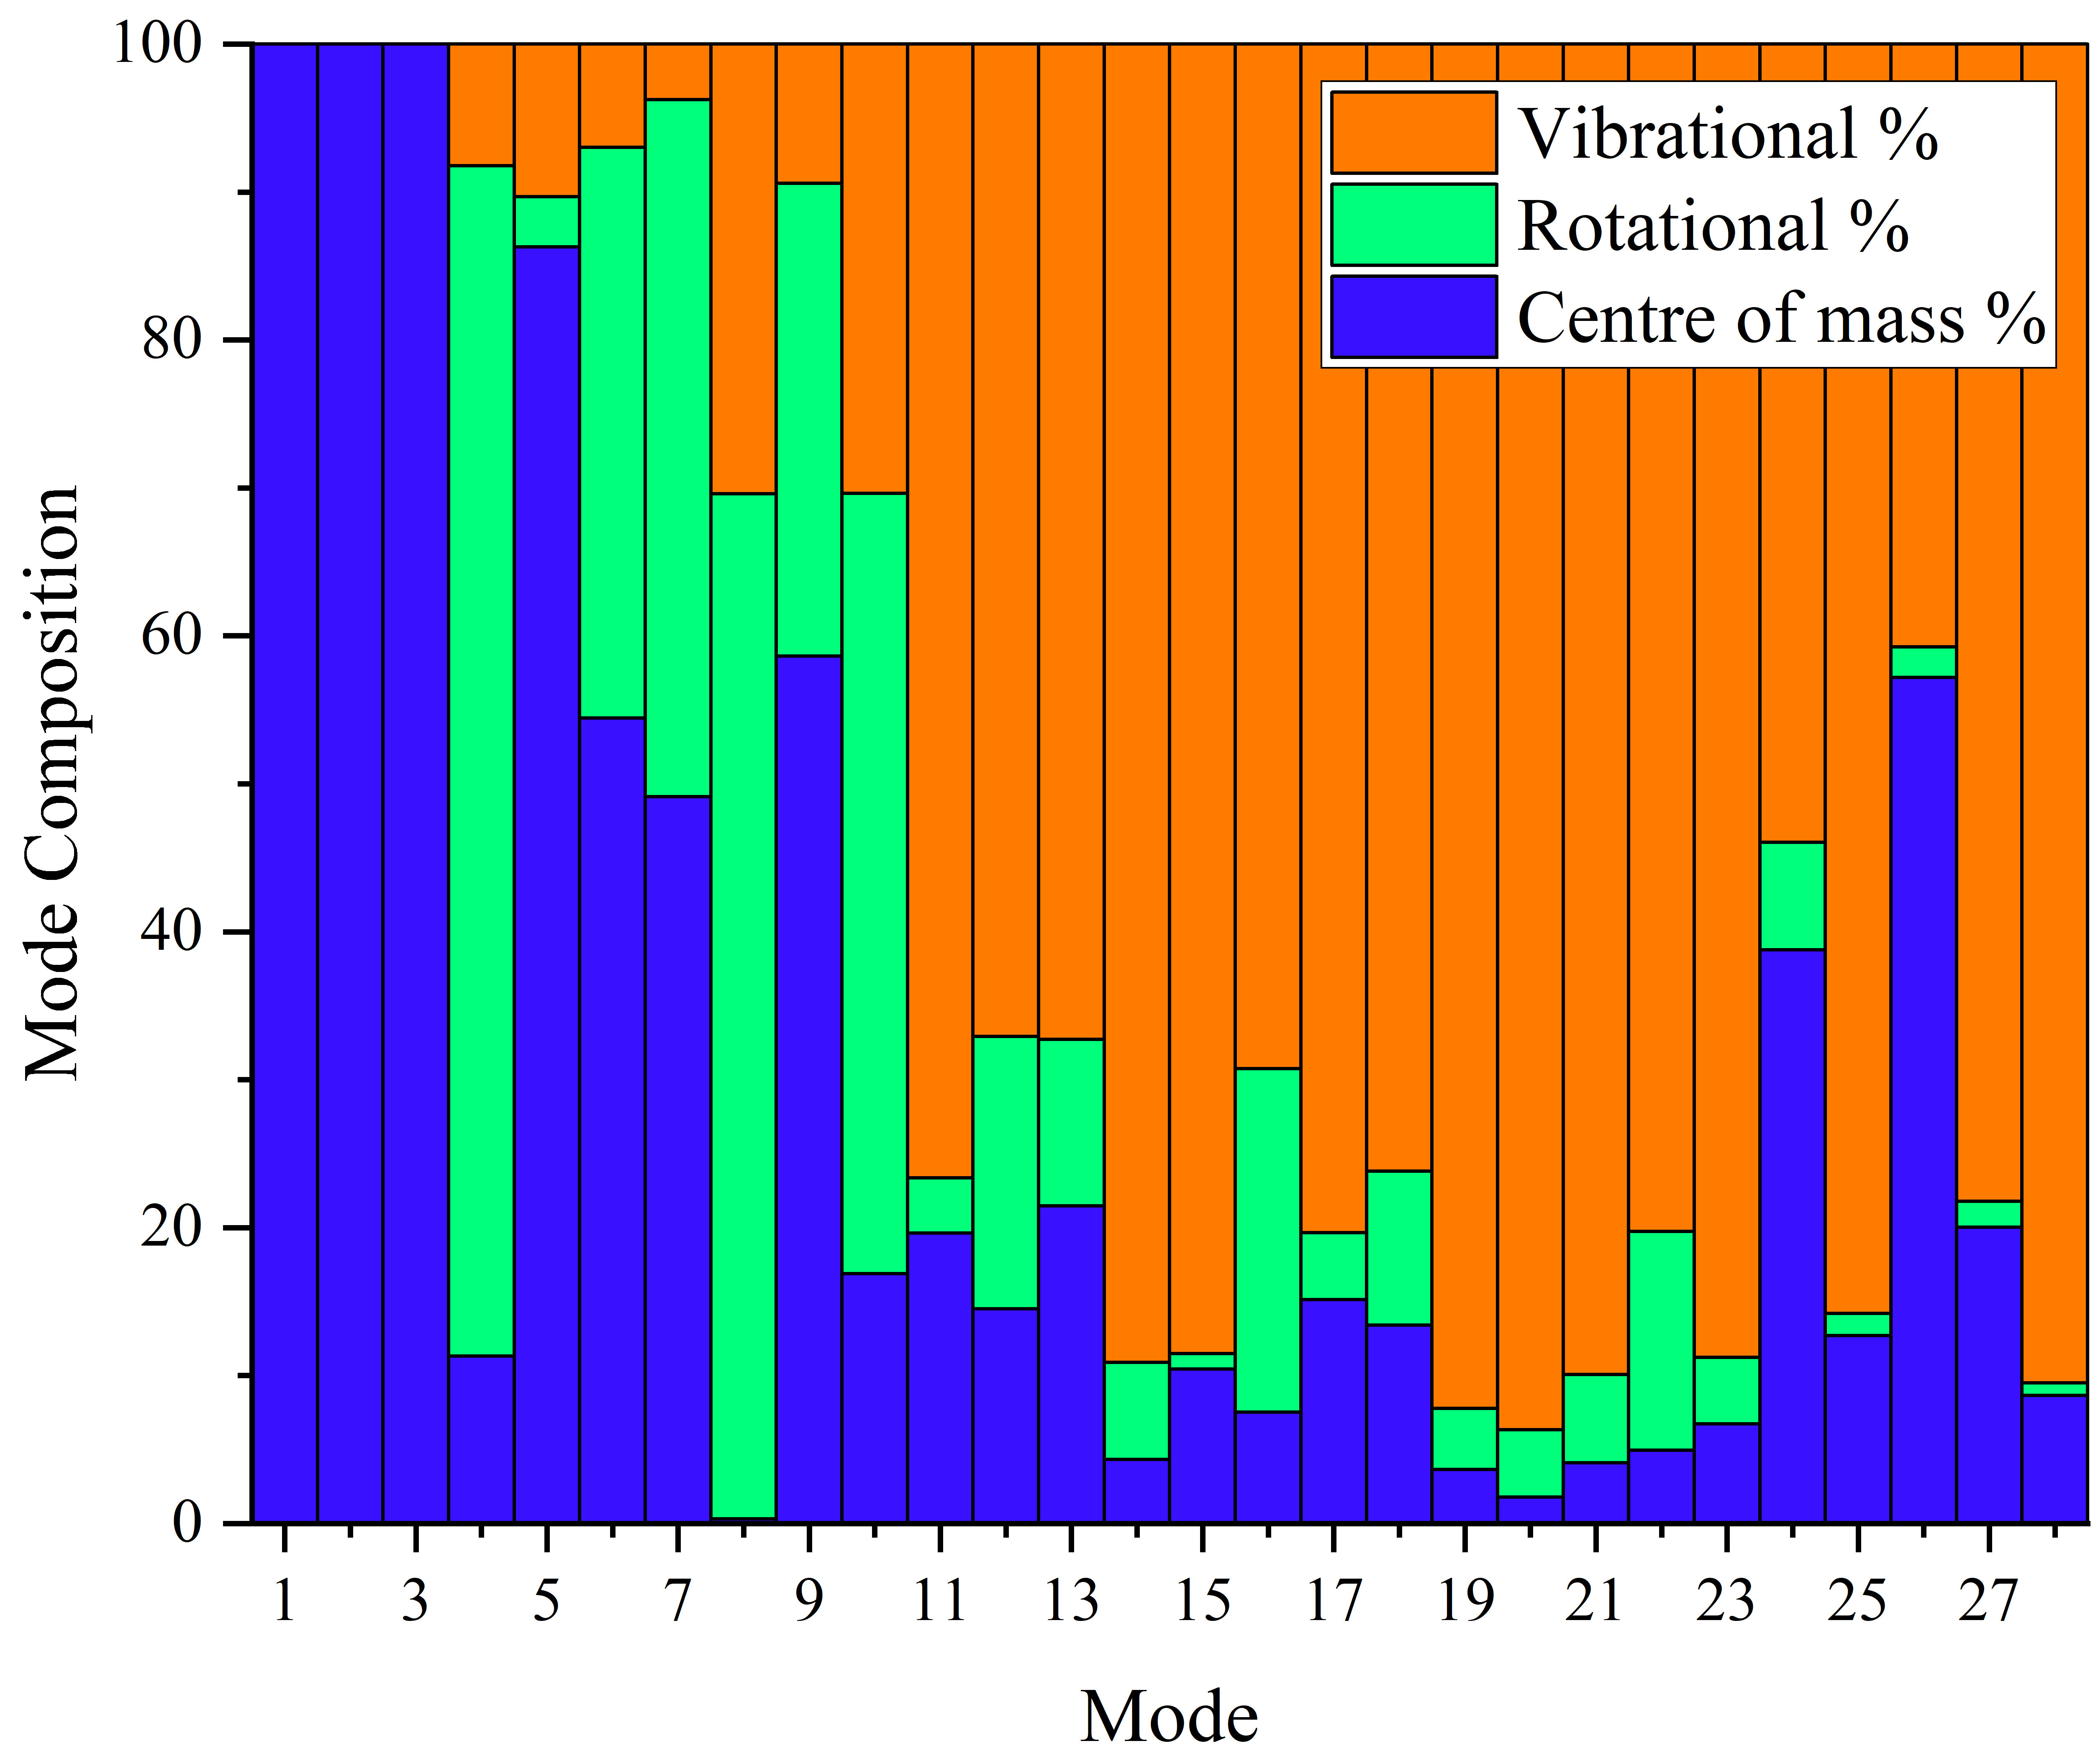
\includegraphics[scale=0.5]{Figures/Analysis/IVDW/D3ModeAnalG.png}
    \caption{D3 Mode Analysis}
    \label{fig:d3_mode_anal}
\end{subfigure}
\captionsetup{font = footnotesize, justification = centering}
\caption[The Mode Composition of \(\alpha\)-Lactose Monohydrate]{The mode composition of \(\alpha\)-Lactose Monohydrate, calculated with PDielec. Both corrections produced very similar histograms indicating the underlying motions making up the modes is not particularly effected by choice of \acrshort{dc}.}
\label{fig:mode_anal}
\end{figure}

When attempting to interpret the calculated modes in the \acrshort{thz} range, it is important to define how the motions of the modes are broken down. The modes in this range do not consist of one kind of motion but are made up of varying amounts of translational, rotational and vibrational components where translational and rotational are considered to be external modes and vibrational is considered to be internal. Unlike in non-periodic systems, the internal and external modes do not have a clear separation \DIFdelbegin \DIFdel{~}\DIFdelend \cite{Jepsen2007} so the further breakdown is necessary. PDielec allows for the breakdown of each mode. The histograms are shown for the D2 and D3 corrections in \Cref{fig:mode_anal}. Whilst there are some small discrepancies between them, they are largely very similar indicating that the corrections themselves did not have a significant effect on the types of phonon modes present and does not affect the order that each phonon appears on the spectrum. These graphs demonstrate the unclear boundary between internal and external modes in the \acrshort{thz} frequency range as the lower frequency external modes all have some vibrational character and the higher frequency internal modes have some rotational and translational character. This is clearly shown by modes 24 and 26 having a significant translational component.

\begin{figure}[t]
    \centering
    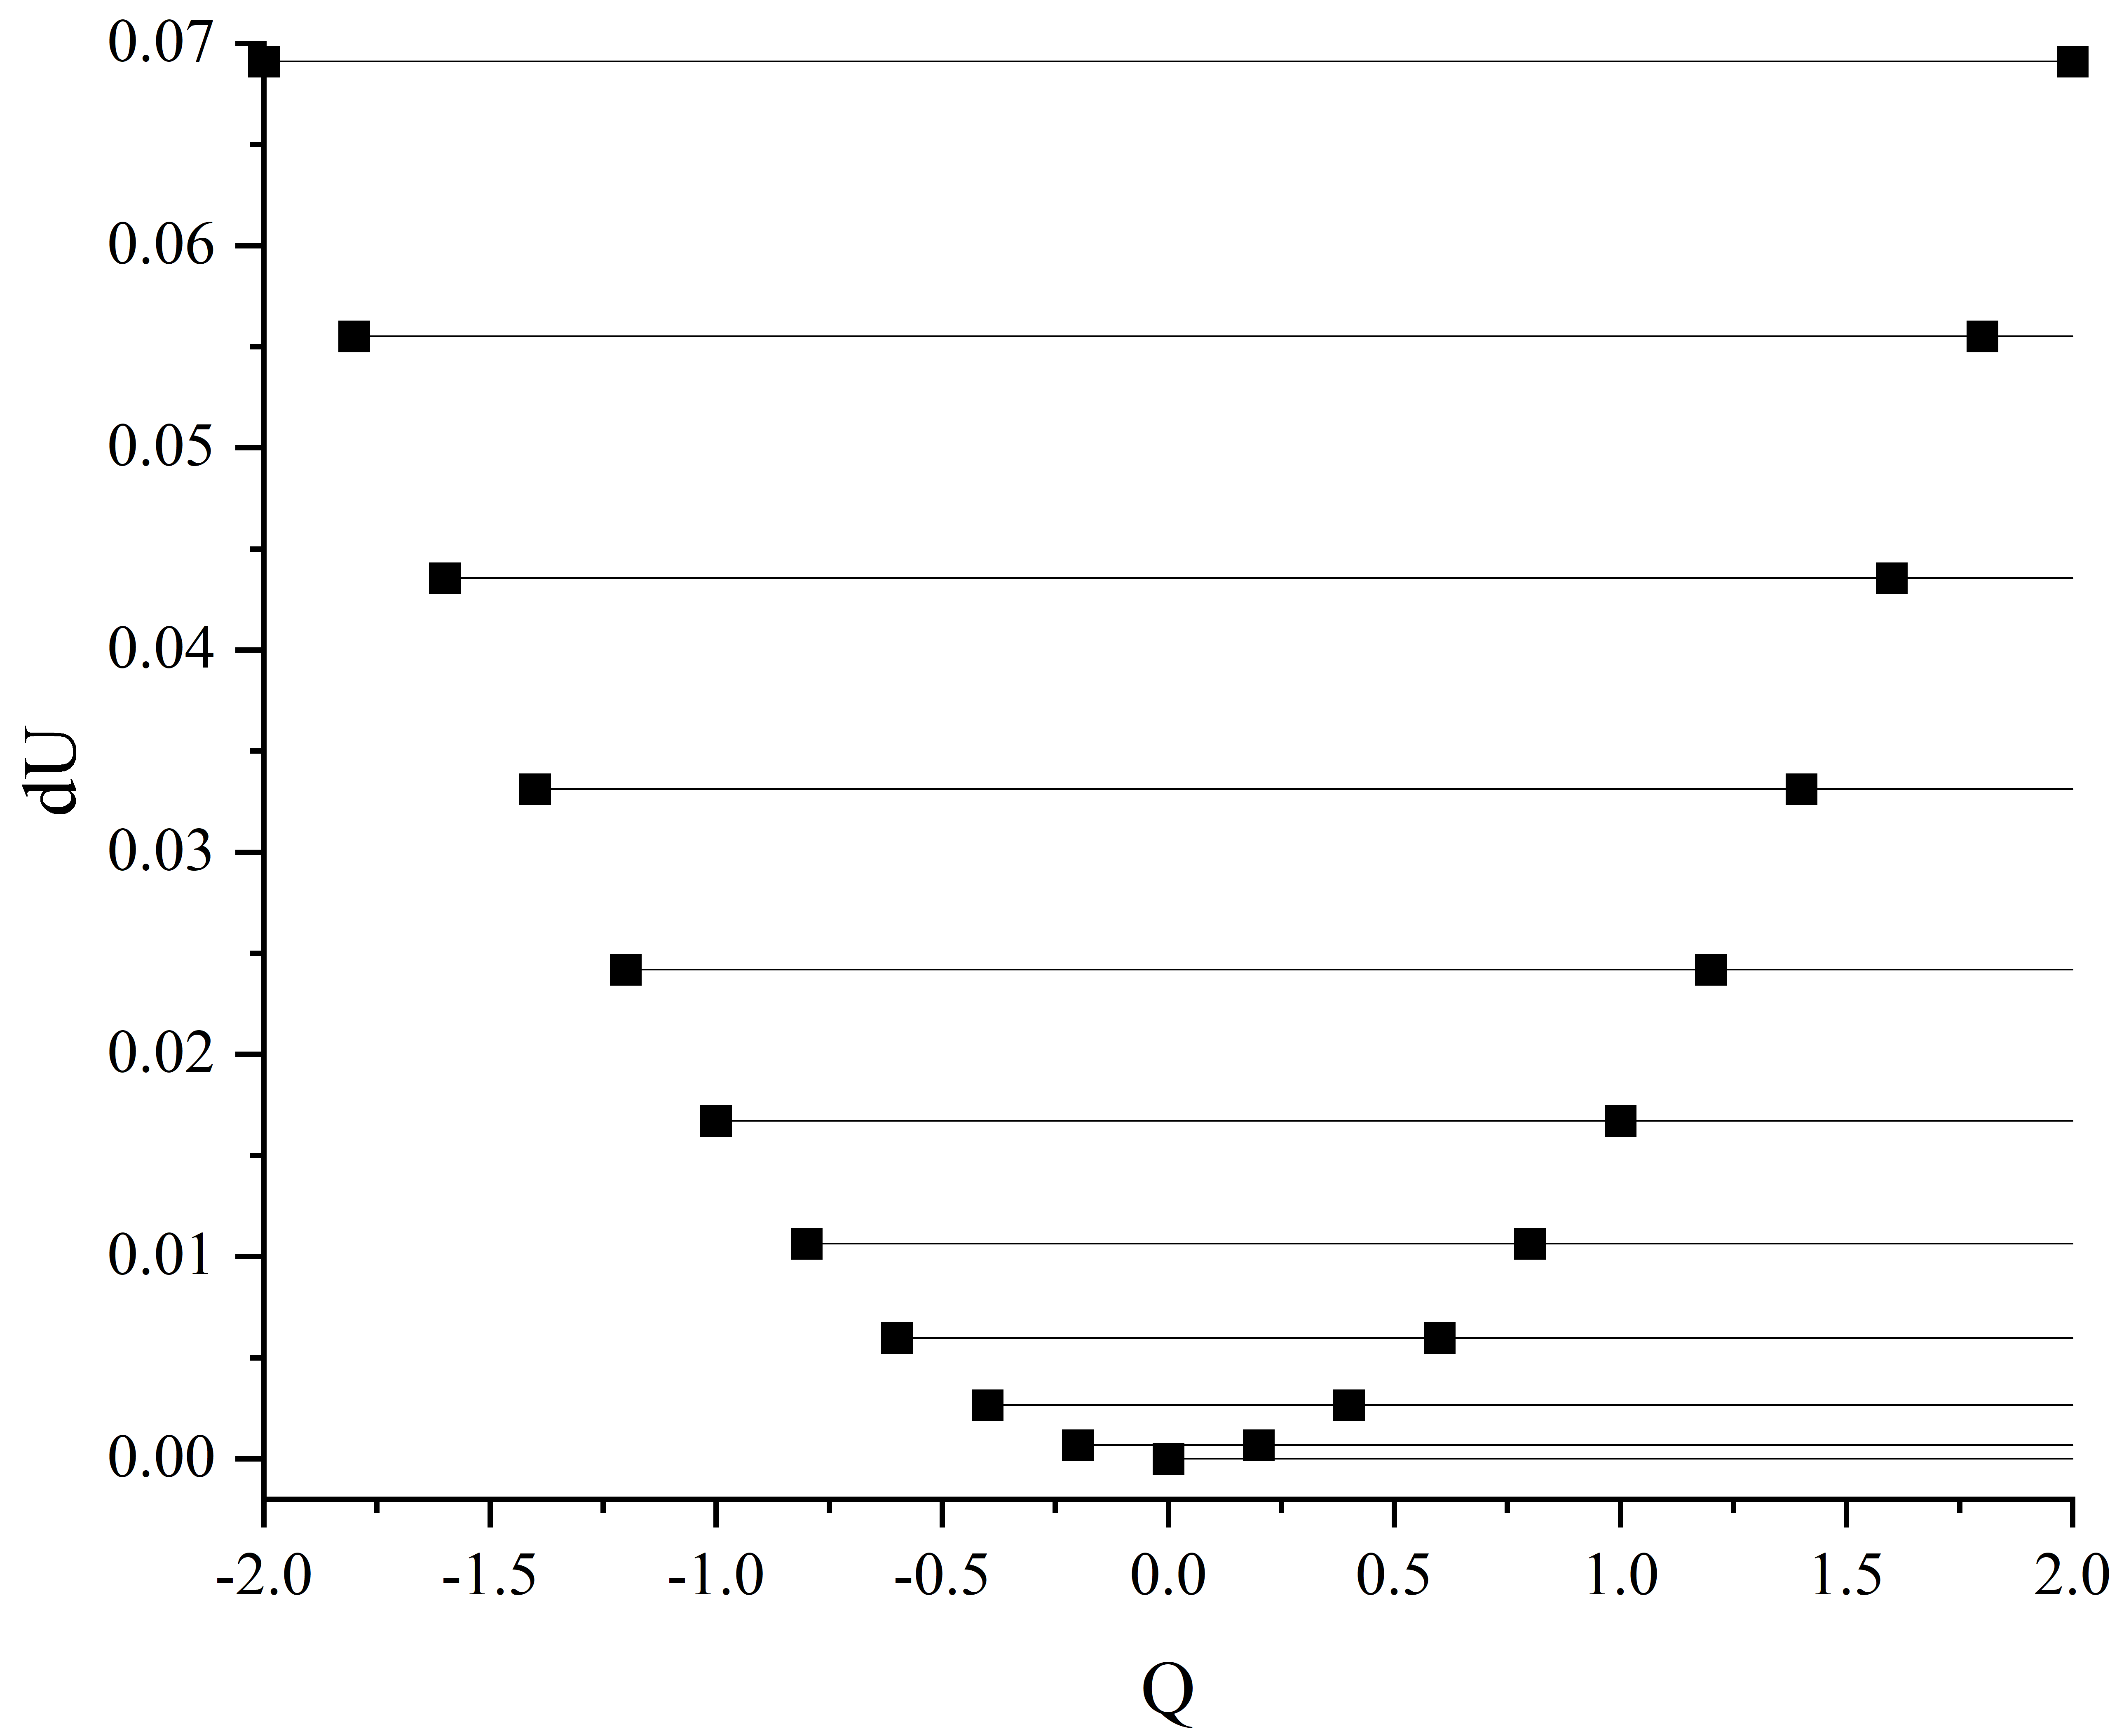
\includegraphics[width=0.7\textwidth]{Figures/Analysis/IVDW/mode13.png}
    \captionsetup{font = footnotesize, justification = centering}
    \caption[The Mode which shows the Largest Discrepancy between Calculation and Experiment]{The mode at \SI{90}{cm^{-1}} which shows the largest discrepancy between calculation and experiment. It can be seen in the top right where the OH groups are moving into each other which may not be represented well by the harmonic approximation.}
    \label{fig:mode13_anharm}
\end{figure}

Whilst these histograms provide information about the breakdown between internal and external modes, they do not provide information about the breakdown of the vibrational components themselves. Using the vibanalysis \DIFdelbegin \DIFdel{~}\DIFdelend \cite{Teixeira2018VMARD} package provided in PDielec, where the motion of a vibrational mode is broken up and the most prominent groups of atomic motions are presented with their respective weights. These groups are bond vibrations, angular motions between three atoms and torsional motions between four atoms. This confirmed the findings from the mode analysis of PDielec that the phonon modes themselves are very similar with only very slight differences which could contribute to the differences in frequencies. However, the findings from this package should only be used in conjunction with the other tools shown above as it was designed for the mid\nobreakdash-\acrshort{ir} region. In that region, there are fewer different types of motion occurring in a single mode and in the \acrshort{thz} frequency range this calculates hundreds of contributions for each mode. 

Finally, the mode at approximately \SI{90}{cm^{-1}} shows the largest discrepancy between calculation and experiment and is shown in \Cref{fig:mode13_anharm}. This could suggest that this mode has a higher degree of anharmonicity than the other modes which could be explained by the motion of the \(O\)\nobreakdash--\(H\) groups towards each other. This will disrupt the network of H\nobreakdash-bonds and this may not be represented well under the harmonic approximation. This mode will be examined further in \Cref{ch:qha}.

\section{Investigation into the Repeatability of Density Functional Theory Calculations}
\label{sec:simstud}
As discussed in \Cref{subsubsec:convergence}, the ionic positions are varied until the changes between each step for the total energy and total forces of the system are below a given tolerance. Owing to the nature of how this variation is carried out, the final structure may have minute differences when several optimisations on the same structure are implemented. To ensure that this phenomenon had not impacted the comparison between \acrshort{dc}s, four \DIFdelbegin \DIFdel{separate }\DIFdelend \DIFaddbegin \DIFadd{seperate }\DIFaddend optimisations and calculations of vibrational properties were performed using the D3 correction and the resulting spectra were compared to each other and to the original D3 calculation\DIFdelbegin \DIFdel{. These were performed using the same version of VASP, with identical starting structures and calculation parameters}\DIFdelend . These spectra are shown completely in \Cref{fig:simstudy1} where the only clear difference is the main peak at approximately \SI{115}{cm^{-1}}. However, the calculations that were performed separately from the main correction investigation show excellent agreement. This is confirmed by \Cref{fig:mode_dissim}, where the differences between each calculation are highlighted for the main group of peaks between 105 and \SI{120}{cm^{-1}} and for the final peaks between 150 and \SI{164}{cm^{-1}}. The original calculation shows reasonable agreement with the other results below \SI{125}{cm^{-1}} but this agreement decreases above this frequency. However, the intensities match well with the exception of the main peak at \SI{115}{cm^{-1}}. This is owing to this peak being the result of the overlap between two modes and these modes are closer together in the original calculation. However, the actual differences between these modes for the original and the new calculations are less than \SI{1}{cm^{-1}} and this was determined to be satisfactory for the main \acrshort{dc} investigation. 

\begin{figure}[h]
    \centering
    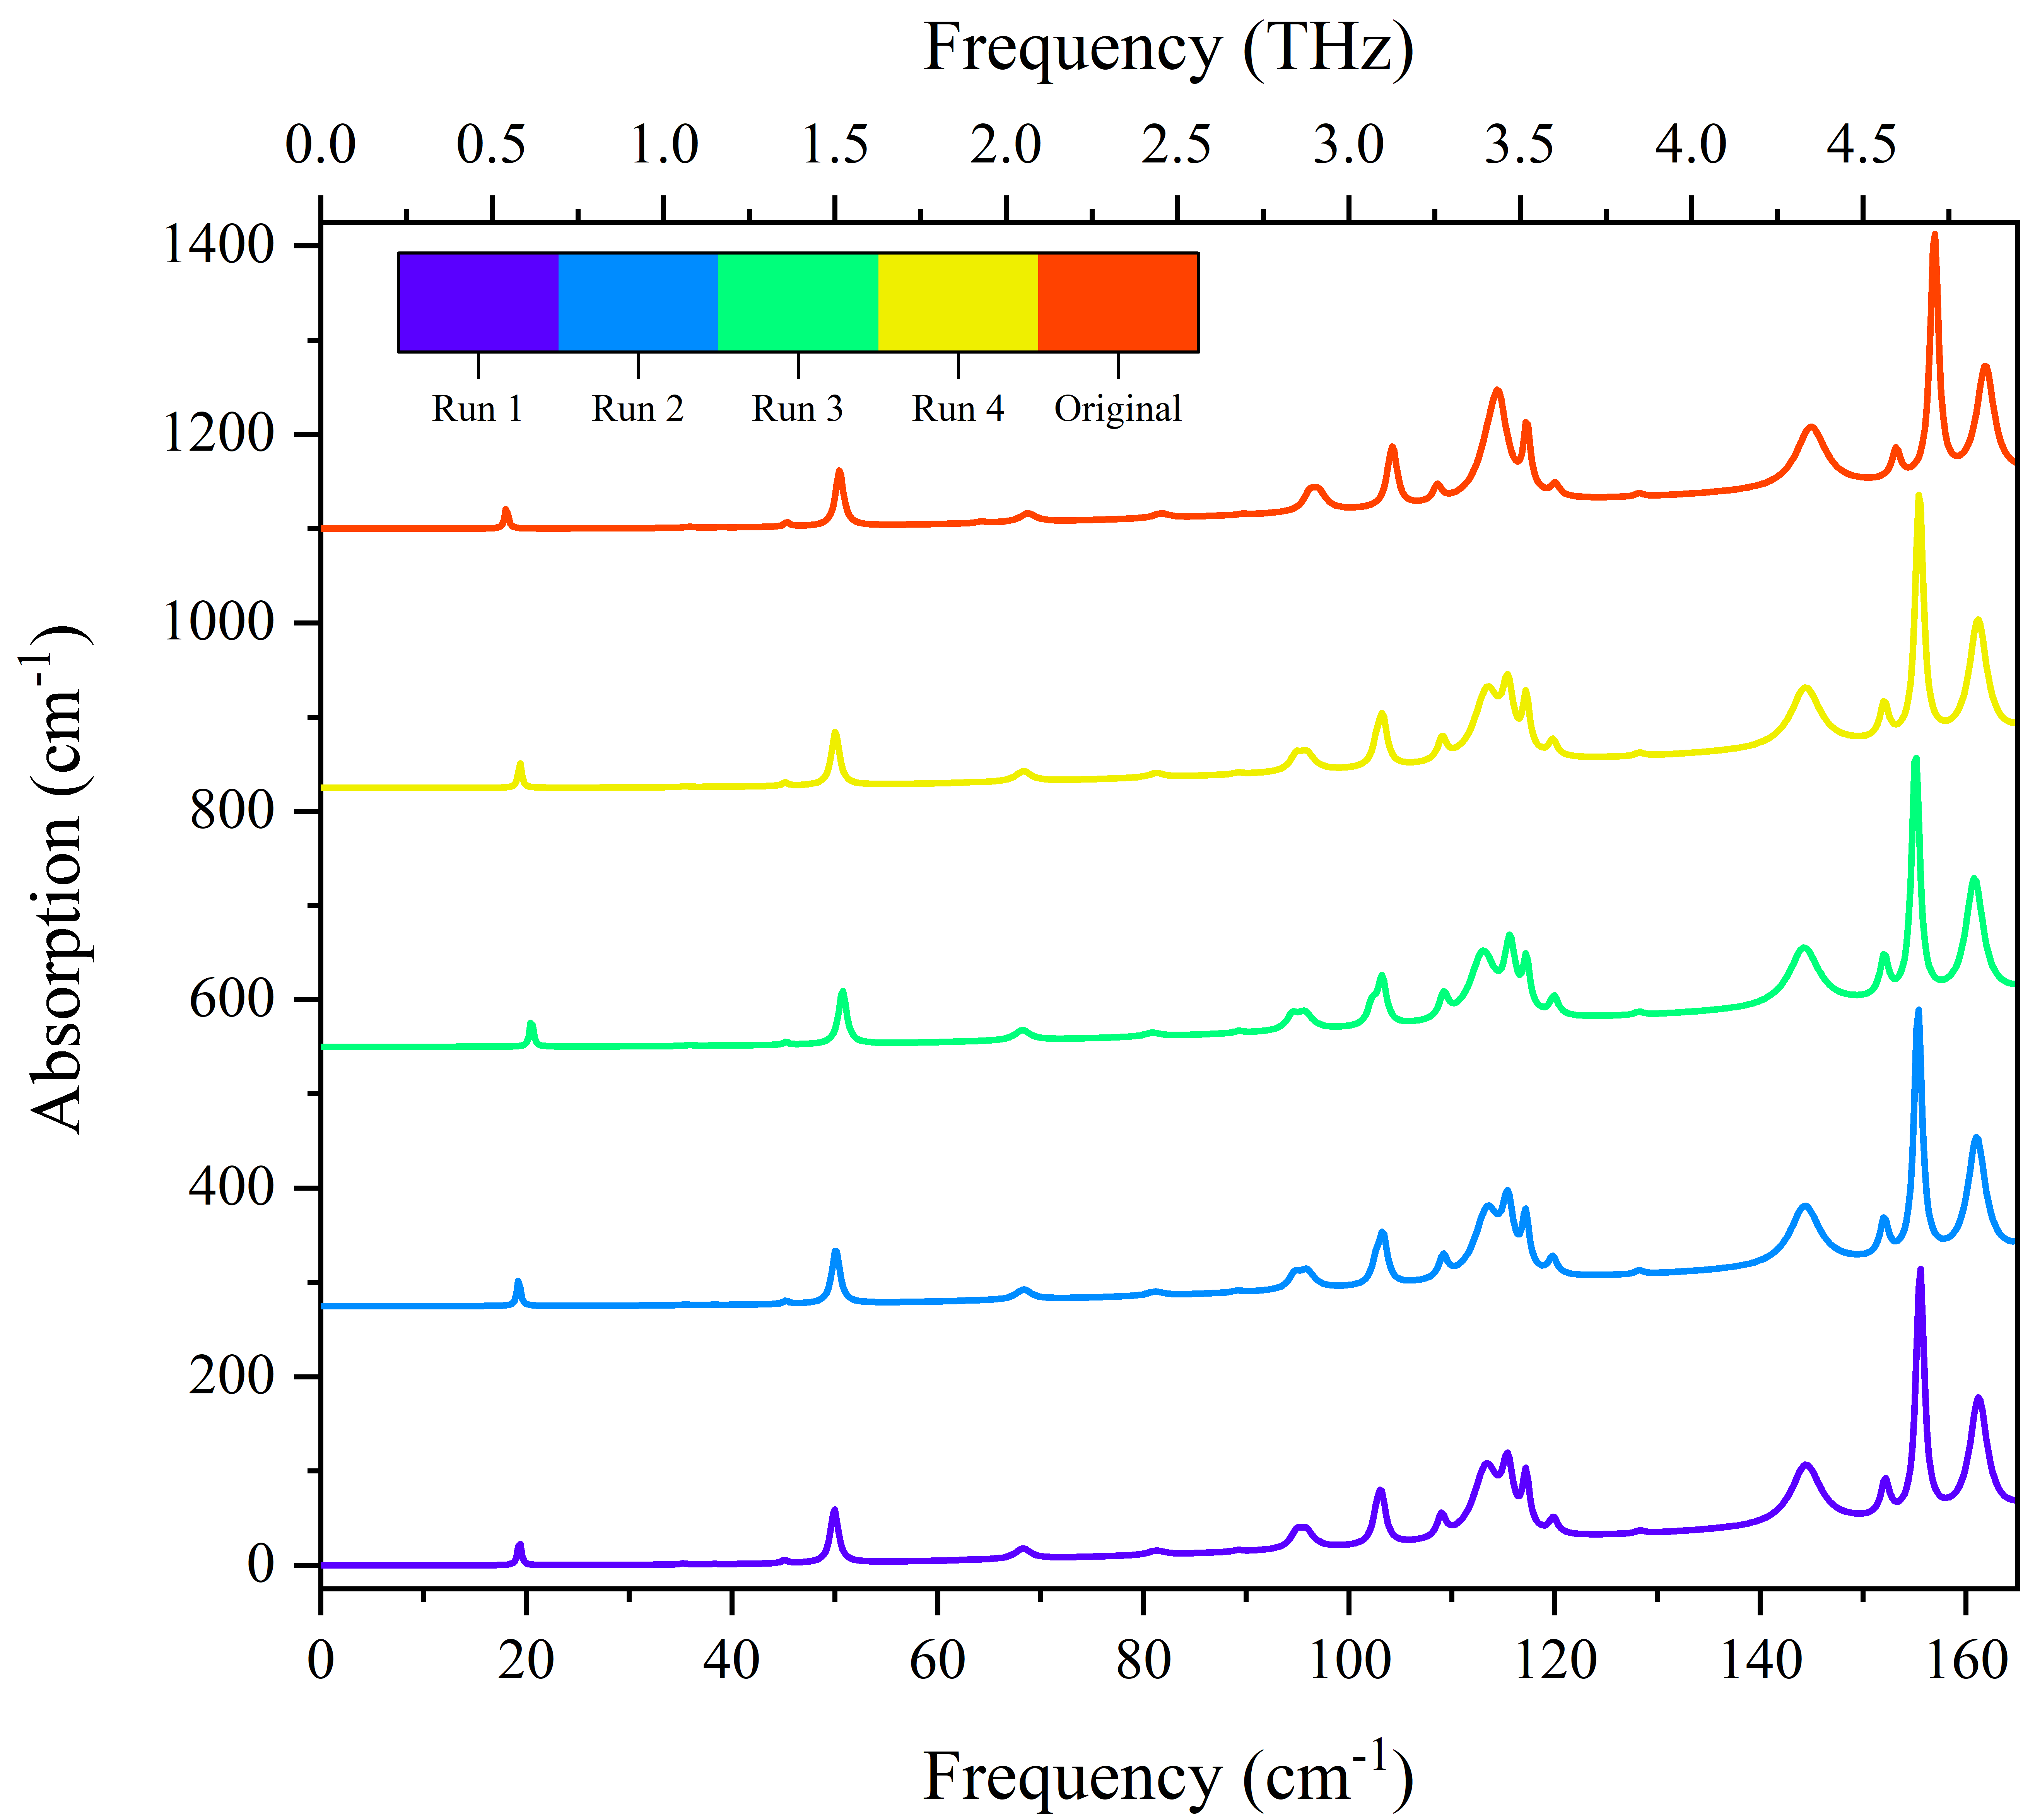
\includegraphics[width=0.7\textwidth]{Figures/Spectra/Sim Study/SimStudG.png}
    \captionsetup{font = footnotesize, justification = centering}
    \caption[The Calculated Terahertz Absorption Spectra of five Optimisations using the D3 Dispersion Correction]{The calculated THz absorption spectra of five separate optimisations using the D3 dispersion correction. With the exception of the peak at approximately \SI{115}{cm^{-1}}, the spectra show reasonably good agreement.}
    \label{fig:simstudy1}
\end{figure}

\begin{figure}
\centering
\begin{subfigure}{\textwidth}
    \centering
    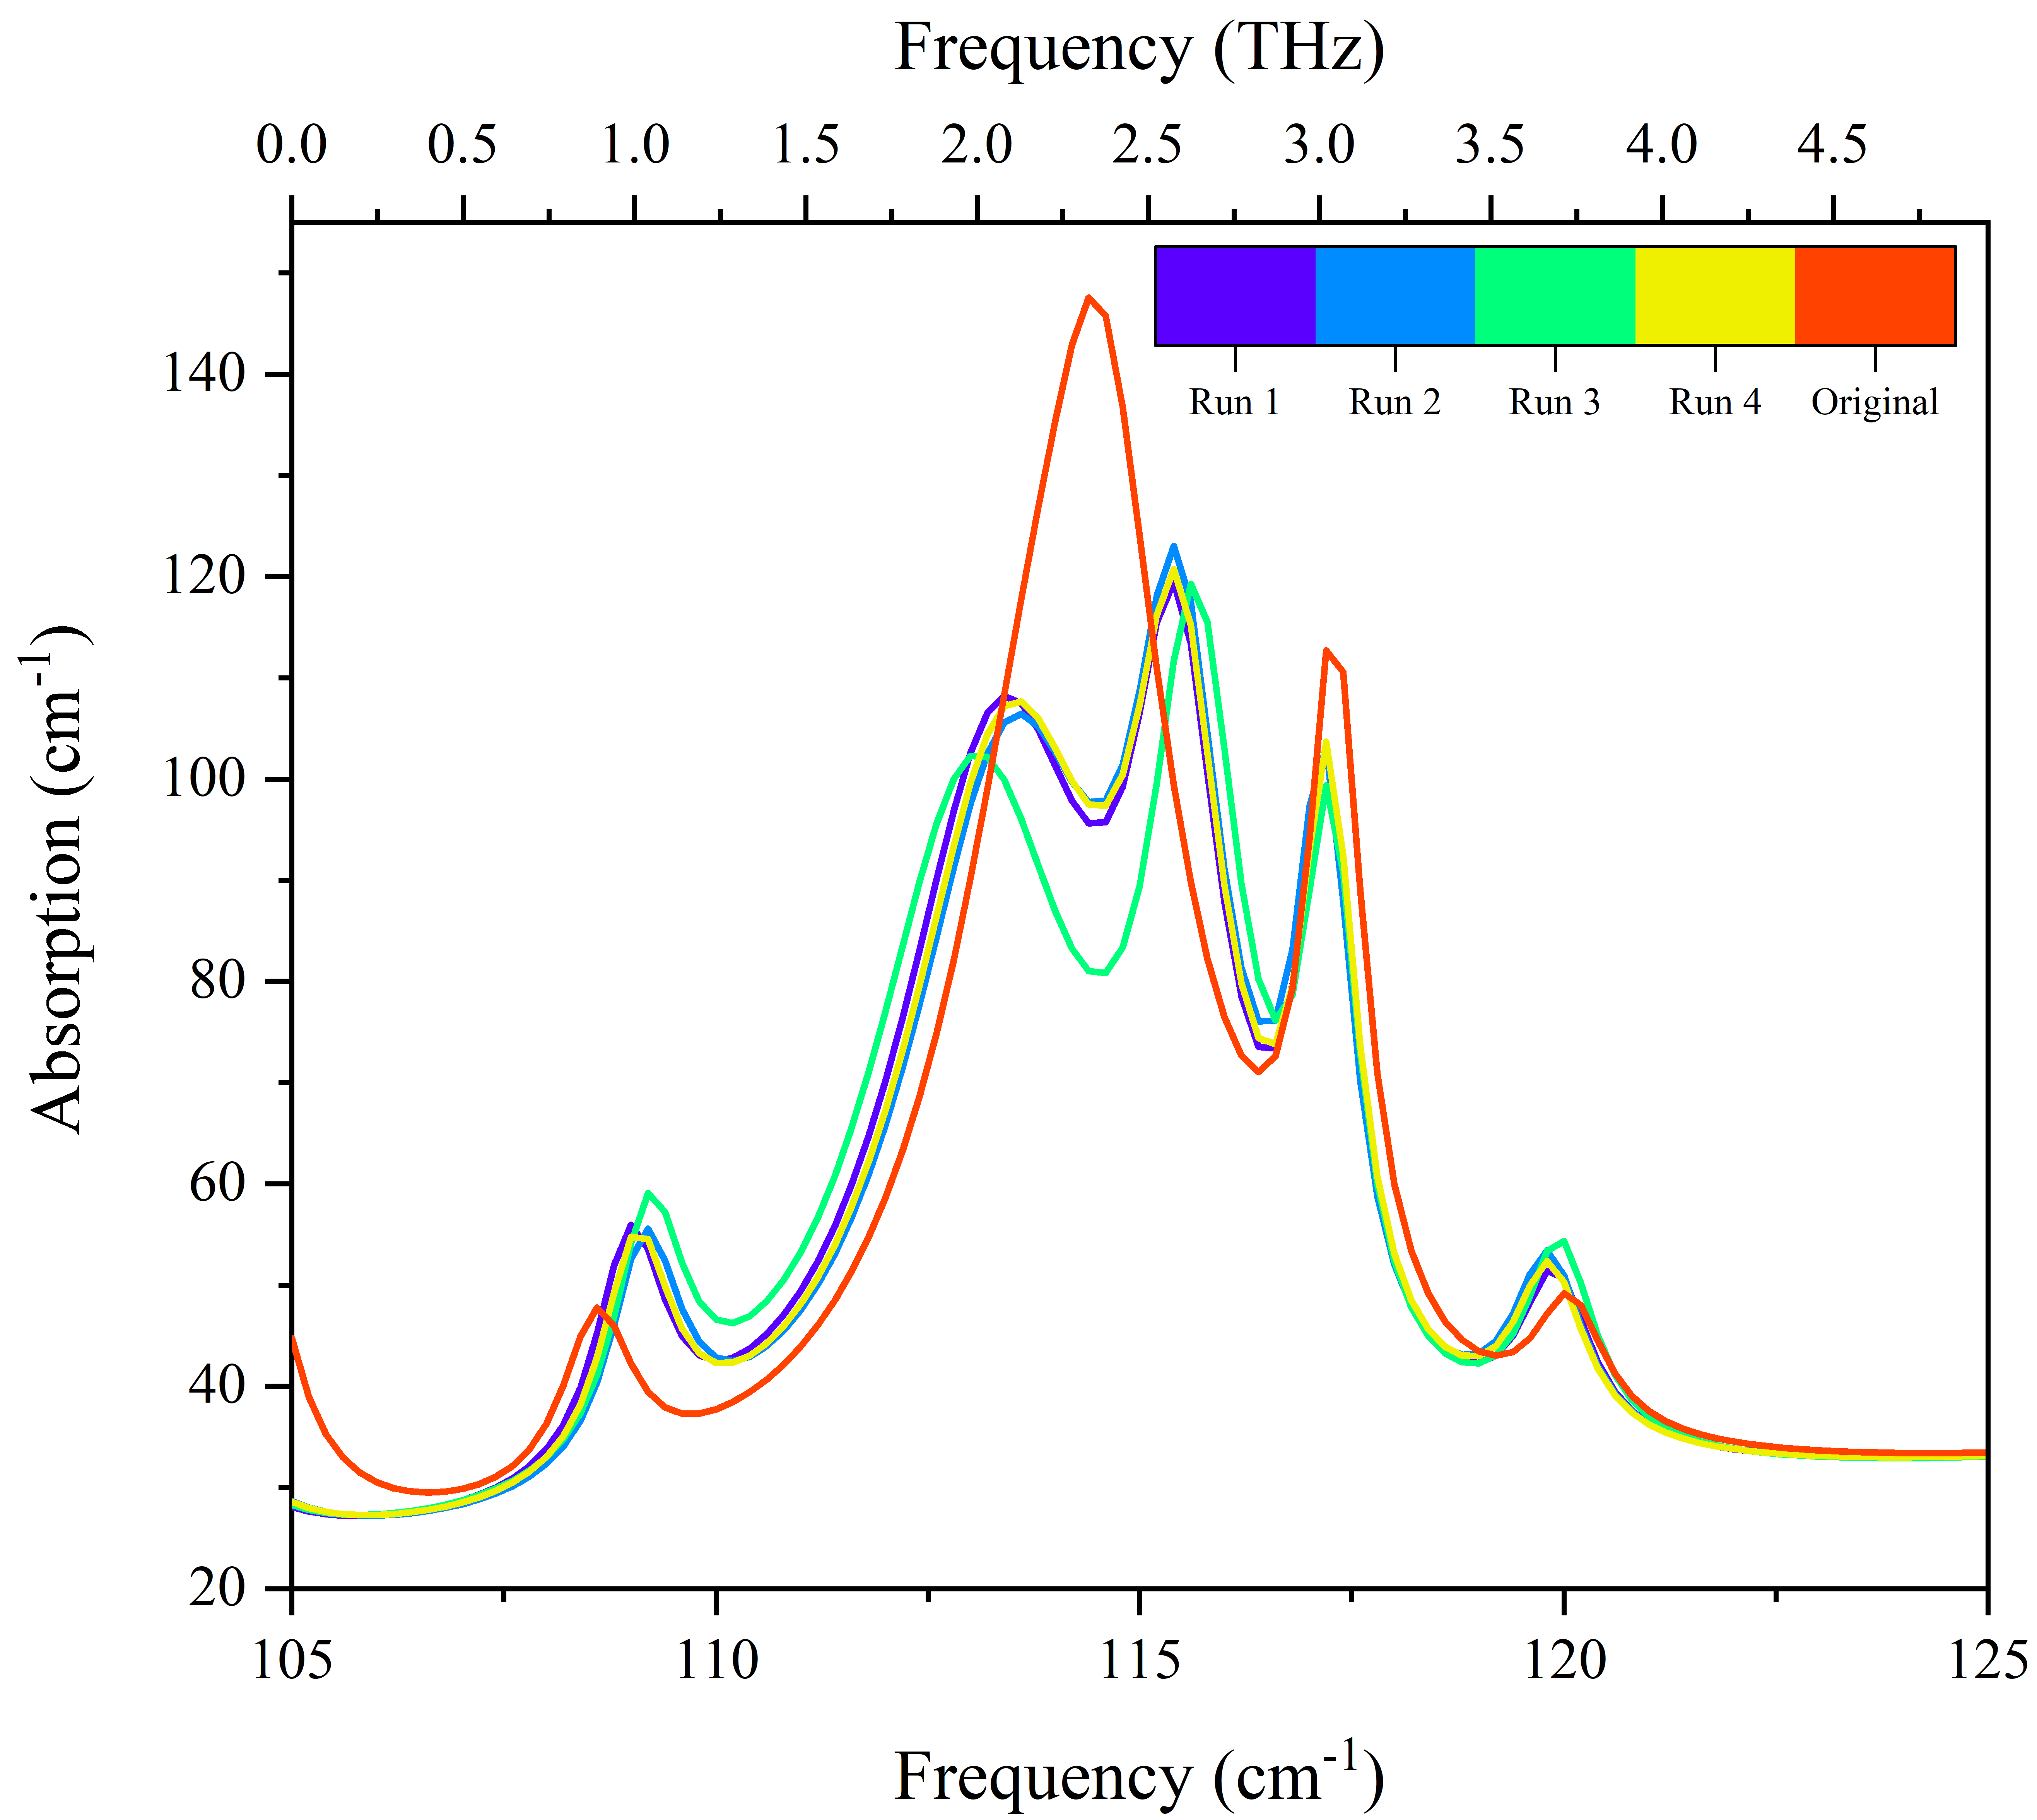
\includegraphics[scale=0.5]{Figures/Spectra/Sim Study/SimStudG2.png}
    \caption{The calculated THz absorption spectra of five separate calculations using the D3 dispersion correction between 105 and \SI{125}{cm^{-1}}.}
    \label{fig:simstudy2}
\end{subfigure}
\begin{subfigure}{\textwidth}
    \centering
    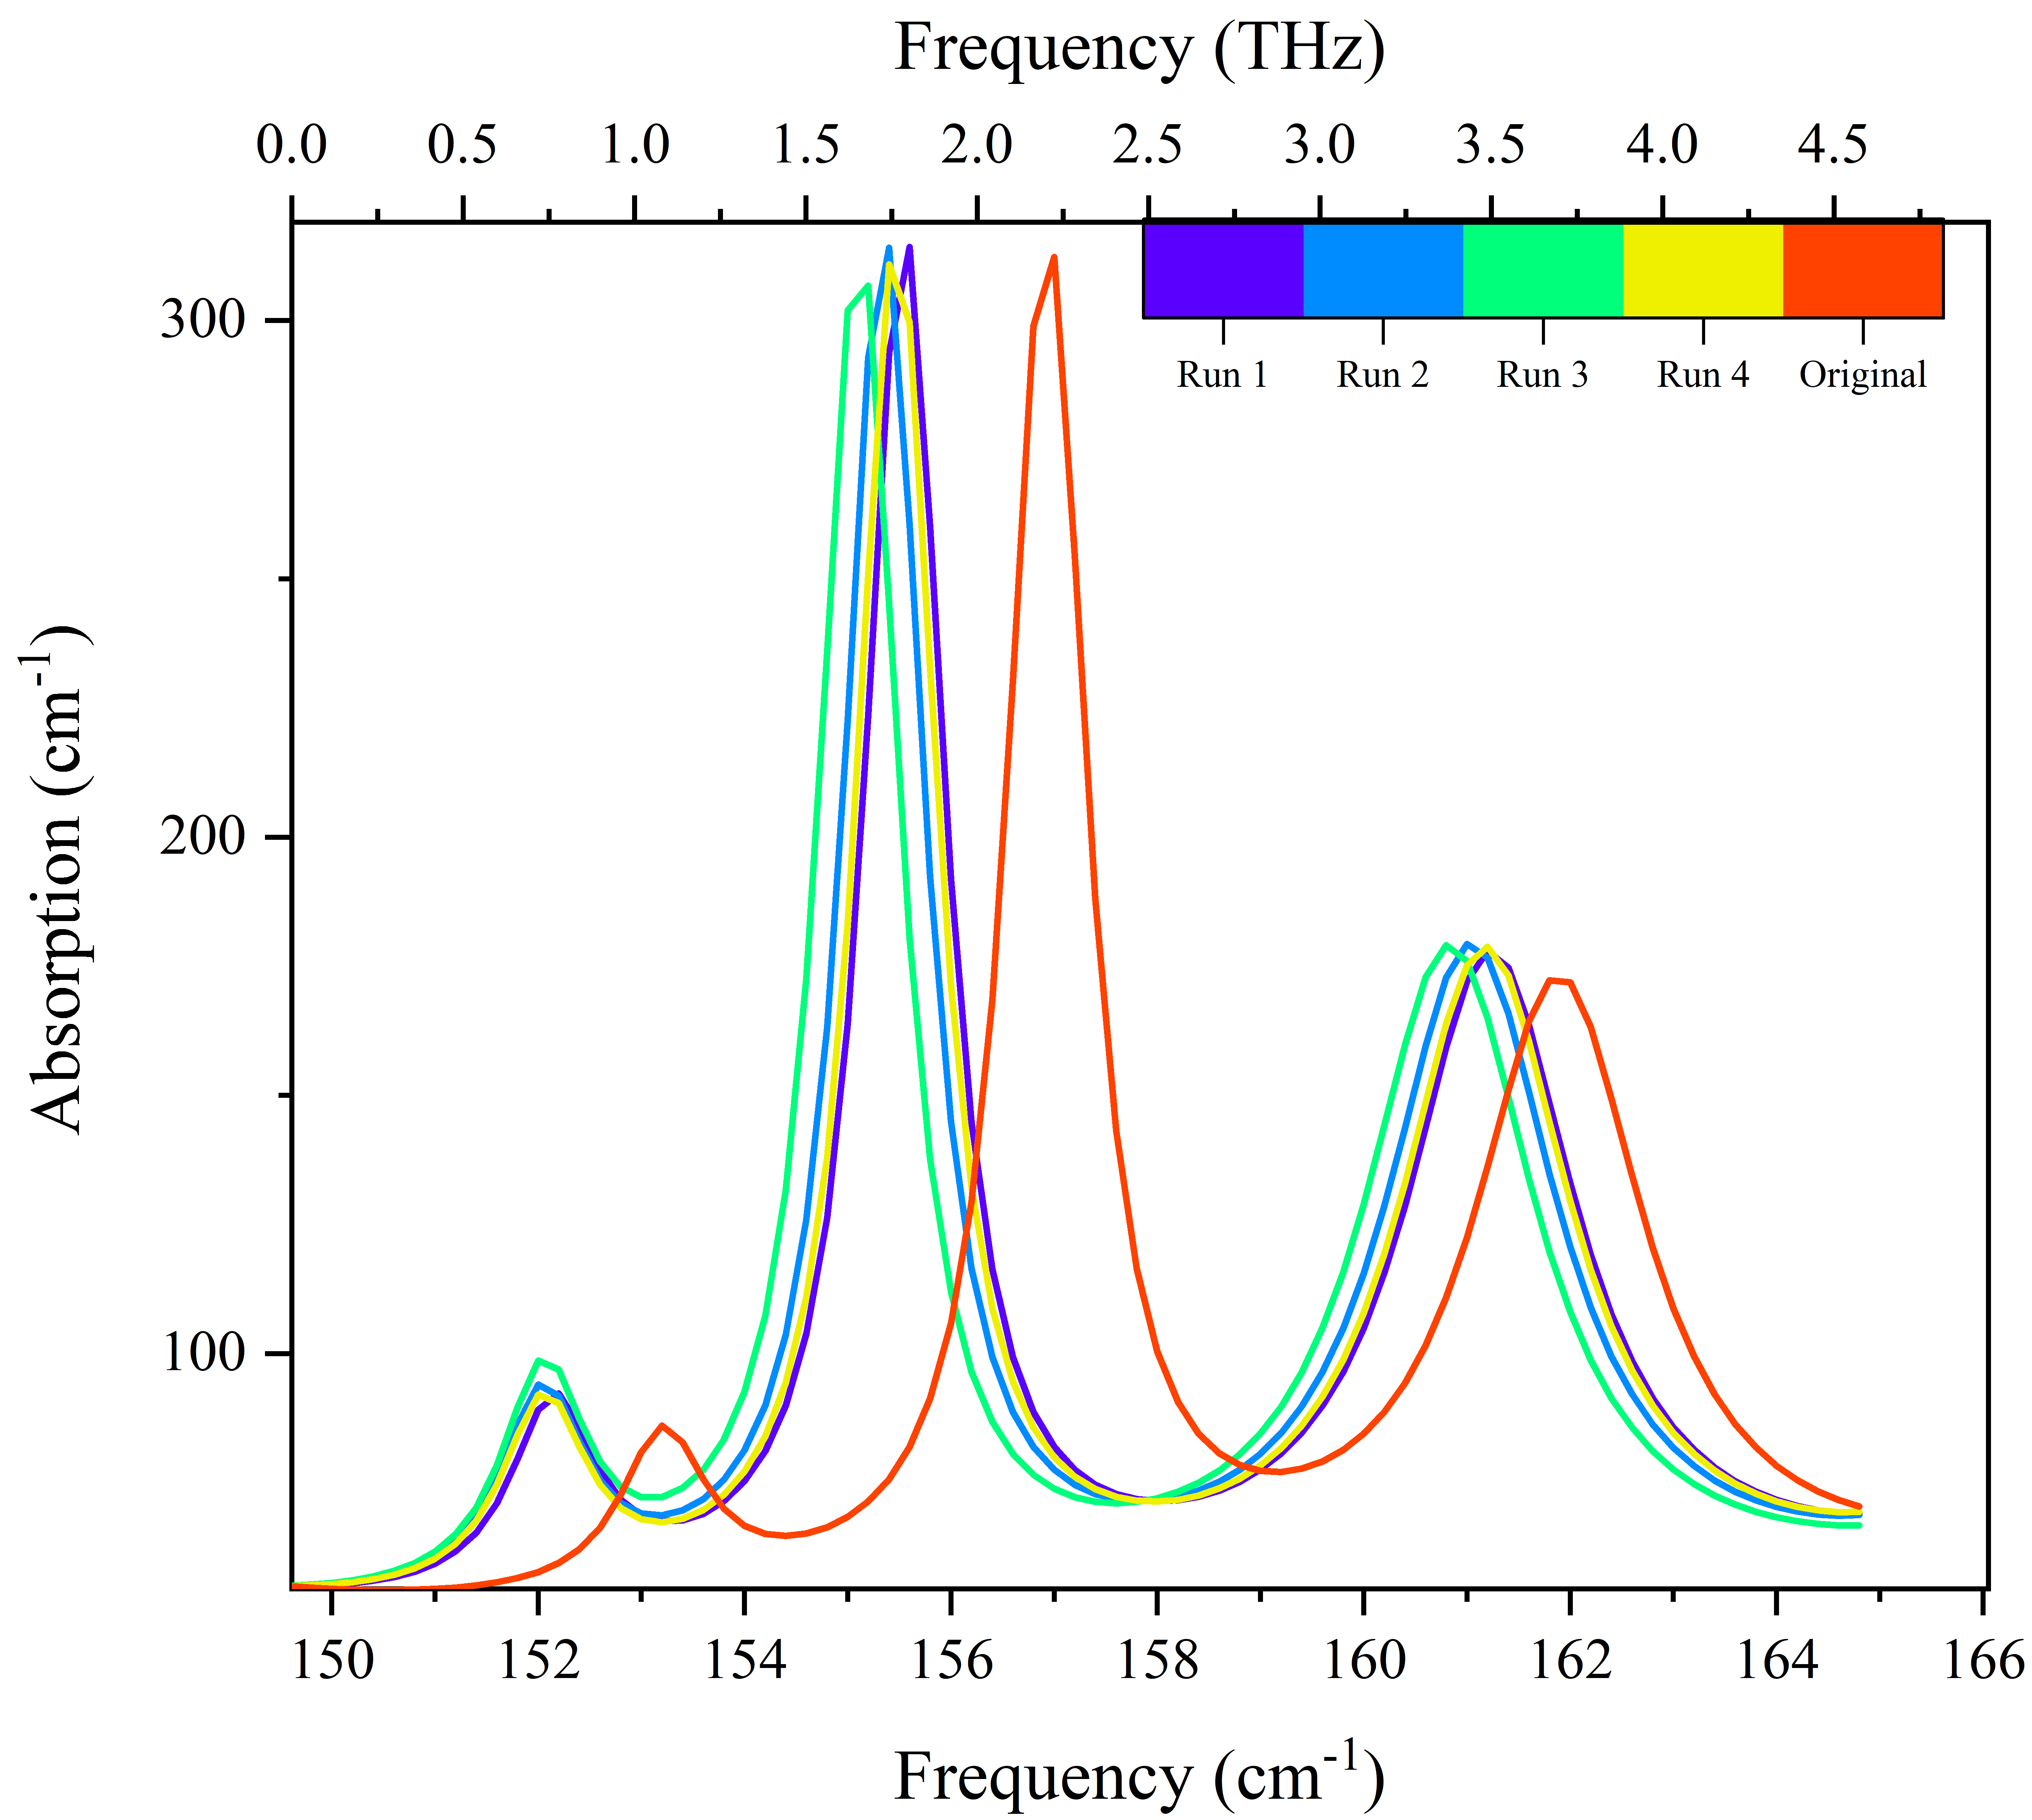
\includegraphics[scale=0.5]{Figures/Spectra/Sim Study/SimStudG3.png}
    \caption{The calculated THz absorption spectra of five separate calculations using the D3 dispersion correction between 150 and \SI{165}{cm^{-1}}.}
    \label{fig:simstudy3}
\end{subfigure}
\captionsetup{font = footnotesize, justification = centering}
\caption[The Differences between the Calculated Terahertz Absorption Spectra of five Optimisations using the D3 Dispersion Correction]{The differences between the calculated THz absorption spectra of five separate optimisations using the D3 dispersion correction.}
\label{fig:mode_dissim}
\end{figure}


\section{Conclusion}
In this chapter, the investigation into the effect of different \acrshort{dc}s was described. This involved performing an optimisation of the structure of \acrshort{alm} and calculating the \acrshort{thz} absorption spectra using the D2, D3, D3\acrshort{bj} and \acrshort{ts} corrections and determining which spectrum best matched the experimental spectrum. A numerical analysis was performed to determine which correction was most suitable for further work on materials such as \acrshort{alm} and other complex organic molecular crystals, and this was found to be the D3 correction although the \acrshort{ts} correction also performed reasonably well. This was achieved through thorough direct comparison of the spectral modes and optimisation of the parameters used in PDielec to construct the spectra. The structural differences were also analysed using several methods to determine what may have caused the spectral differences. Analysis of the modes provided evidence that the dispersion only marginally changes the composition of the phonon modes which is likely the explanation for the differences in mode frequency. However, a definitive correlation between structure and mode position and intensity was not found.
Finally, the repeatability of a calculation was determined through the calculation of four \acrshort{alm} \acrshort{thz} absorption spectra using the D3 correction and these were compared to each other and to the original D3 spectrum. It was determined that below the dynamic range of the system, the differences between these calculations is tolerable.




